%%%%%%%%%%%%%%%%%%%%%%%%%%%%%%%%%%%%%%%%%%%%%%%%%%%%%%%%%%%%%%%%%%%%%%
% LaTeX Template: Project Modified (v 0.2) by jluo
%
% Original Source: http://www.howtotex.com
% Date: February 2019
% 
% This is a title page template which be used for articles & reports.
% 
% 
%%%%%%%%%%%%%%%%%%%%%%%%%%%%%%%%%%%%%%%%%%%%%%%%%%%%%%%%%%%%%%%%%%%%%%

\documentclass[11   pt]{report}
\usepackage[a4paper]{geometry}
\usepackage[myheadings]{fullpage}
\usepackage{fancyhdr}
\usepackage{lastpage}
\usepackage{mdframed}
\usepackage{fourier}
\usepackage{algorithm} 
\usepackage{algpseudocode} 
\usepackage{amsthm}
\usepackage{tcolorbox}
\usepackage{graphicx, wrapfig, subcaption, setspace, booktabs}
\usepackage[T1]{fontenc}
\usepackage[font=small, labelfont=bf]{caption}
\usepackage{fourier}
\usepackage[protrusion=true, expansion=true]{microtype}
\usepackage[english]{babel}
\usepackage{amsmath,amssymb}
\usepackage{sectsty}
\usepackage{url, lipsum}
\usepackage{tgbonum}
\usepackage{hyperref}
\newtheorem{theorem}{Theorem}[section]
\newtheorem{corollary}{Corollary}[theorem]
\newtheorem{lemma}[theorem]{Lemma}
\usepackage{xcolor}
\usepackage{listings}
\usepackage{color}
\usepackage{tocloft}

% TOC Formatting
\setlength{\cftpartindent}{0em}           % No indentation for parts
\setlength{\cftchapindent}{1.8em}         % Chapter indentation under parts
\setlength{\cftsecindent}{3.8em}          % Section indentation under chapters
\setlength{\cftsubsecindent}{5.8em}       % Subsection indentation

% Vertical spacing
\setlength{\cftbeforepartskip}{15pt}      % Space before each part
\setlength{\cftbeforechapskip}{8pt}       % Space before each chapter
\setlength{\cftbeforesecskip}{4pt}        % Space before each section

% Font styling
\renewcommand{\cftpartfont}{\large\scshape\bfseries}
\renewcommand{\cftpartpagefont}{\large\bfseries}
\renewcommand{\cftchapfont}{\normalsize\bfseries}
\renewcommand{\cftchappagefont}{\normalsize}


 \usepackage{amsfonts,mathrsfs}
\definecolor{codegreen}{rgb}{0,0.6,0}
\definecolor{codegray}{rgb}{0.5,0.5,0.5}
\definecolor{codepurple}{rgb}{0.58,0,0.82}
\definecolor{backcolour}{rgb}{0.95,0.95,0.92}
 
\lstdefinestyle{mystyle}{
    backgroundcolor=\color{backcolour},   
    commentstyle=\color{codegreen},
    keywordstyle=\color{magenta},
    numberstyle=\tiny\color{codegray},
    stringstyle=\color{codepurple},
    basicstyle=\footnotesize,
    breakatwhitespace=false,         
    breaklines=true,                 
    captionpos=b,                    
    keepspaces=true,                 
    numbers=left,                    
    numbersep=5pt,                  
    showspaces=false,                
    showstringspaces=false,
    showtabs=false,                  
    tabsize=2
}
 
\lstset{style=mystyle}
% --- Define theorem environments ---
\newtheorem{definition}{Definition}[section]

% --- Box style for definitions ---
\newmdenv[
  linewidth=0.8pt,     % thickness of box border
  roundcorner=2pt,     % small rounded corners
  skipabove=10pt,      % vertical space before box
  skipbelow=10pt       % vertical space after box
]{defbox}

% --- Environment for boxed definitions ---
\newenvironment{boxeddefinition}[1][] % optional argument for title
  {\begin{defbox}\begin{definition}[#1]}
  {\end{definition}\end{defbox}}


\newcommand{\HRule}[1]{\rule{\linewidth}{#1}}
\onehalfspacing
\setcounter{tocdepth}{5}
\setcounter{secnumdepth}{5}
\usepackage[numbers]{natbib}  % Enable numeric citations

\bibliographystyle{abbrvnat}
\bibpunct{,}{}{;}{a}{}{}  % to get correct punctuation for bibliography
\setlength{\skip\footins}{1.5cm}
\newcommand{\citets}[1]{\citeauthor{#1}'s \citeyearpar{#1}}
\renewcommand\bibname{References}  
%-------------------------------------------------------------------------------
% HEADER & FOOTER
%-------------------------------------------------------------------------------
%\pagestyle{fancy}
%\fancyhf{}
%\setlength\headheight{15pt}
%\fancyhead[L]{Student ID: 1034511}
%\fancyhead[R]{Anglia Ruskin University}
%\fancyfoot[R]{Page \thepage\ of \pageref{LastPage}}
%-------------------------------------------------------------------------------
% TITLE PAGE
%-------------------------------------------------------------------------------

\begin{document}
{\fontfamily{cmr}\selectfont
\title{ 
    \normalsize \textsc{}
    \\ [1.0cm]
    \HRule{0.5pt} \\
    \centering
    \large \textbf{\uppercase{Valuation of Financial Derivatives under X-Value Adjustments using Deep Learning Techniques}} \\  % Using \large instead of \Large
    \HRule{0.5pt} \\ [0.3cm]
    \normalsize \today \\
    \vspace*{2\baselineskip}
}

\date{}

\author{
		Lindani Melusi Hlophe \\ 
		Student Number: 2579491\\}

\maketitle
% --- ABSTRACT ---
\begin{abstract}
\addcontentsline{toc}{chapter}{Abstract}
This study develops deep learning surrogate models for the direct computation of Credit Valuation Adjustment (CVA) and Debit Valuation Adjustment (DVA) for an interest rate swap (IRS) under the Hull-White one-factor model. Standard xVA computation requires a nested Monte Carlo simulation in which the outer loop evolves the short rate along simulated paths and the inner loop re-prices the derivative at each monitoring date and scenario. This nested structure grows rapidly in computational cost with the number of scenarios and monitoring dates, and hence creates a computational bottleneck. We address this by training two differential deep learning surrogates to directly approximate the Expected Positive Exposure (EPE) and Expected Negative Exposure (ENE) profiles as explicit functions of the initial yield curve, Hull-White parameters, and monitoring time. Since EPE and ENE are already expectations over the short rate distribution, the short rate itself does not appear as a surrogate input, and CVA and DVA are recovered at inference time through a single forward pass per monitoring date with no simulation. Each surrogate is trained jointly on exposure values and their analytic curve sensitivities, which regularizes the learned function and improves accuracy under yield curve shapes not well represented in the training distribution. The trained surrogates reproduce EPE, ENE, CVA, and DVA estimates consistent with a full Monte Carlo benchmark across a range of yield-curve environments, whilst eliminating simulation cost during inference. These results establish that the deep learning surrogates offer a practically viable approach to xVA computation, and the framework is sufficiently general to extend to instruments with more complex payoff structures.
 % Your abstract content
\end{abstract}

\newpage

% --- FRONT MATTER LISTS ---
\listoffigures
\addcontentsline{toc}{chapter}{List of Figures}

\newpage
\listoftables
\addcontentsline{toc}{chapter}{List of Tables}

\newpage
\chapter*{Acronyms}
\addcontentsline{toc}{chapter}{Acronyms}
% Content for acronyms goes here or \input{acronyms}

\newpage
\chapter*{Notation}
\addcontentsline{toc}{chapter}{Notation}


\tableofcontents
\newpage

%-------------------------------------------------------------------------------
% Section title formatting
\sectionfont{\scshape}
%-------------------------------------------------------------------------------

%-------------------------------------------------------------------------------
% BODY
%-------------------------------------------------------------------------------
    
\newpage
\part{Introduction and Research Objectives}
    \include{IntroductionAndObjectives}

\part{Theoretical Foundations}
    \chapter{Valuation of Financial Derivatives}
    \noindent
    This chapter establishes the mathematical framework underpinning the valuation of financial derivatives. Financial derivatives pricing heavily relies on stochastic calculus to model the random evolution of asset prices and derive prices free of arbitrage \cite{hirsa2013introduction}. We consider a continuous-time financial market model over a finite time horizon $T < \infty$, and the uncertainty in the market is modeled by a  probability space.

    \begin{theorem}[Probability Space] \label{thm:probability-space}
         A \textbf{Probability space} is the triple $(\Omega, \mathcal{F}, \mathbb{Q})$, it provides the mathematical structure for defining random processes and modeling the flow of information.
        \begin{itemize}
            \item $\Omega$ is the set of all market states
            \item $\mathcal{F}$ is a sigma-field describing the flow of information over time, represented by a filtration $\mathcal{F}_t$. It contains historical market prices up to time $t$
            \item $\mathbb{Q}$ is the probability measure (often referred to as the risk-neutral measure or real measure $\mathbb{P}$)
        \end{itemize}
    \end{theorem}
    
    \noindent
    The filtration $(\mathcal{F}_t)_{t \in [0,T]}$ formalises this information structure by specifying precisely what is observable at each instant, ruling out any anticipation of future market realisations. Each financial underlying is then modelled as a stochastic process adapted to this filtration, so that its value at time $t$ depends only on information available up to and including $t$. 

     \newpage
    \begin{definition}[Stochastic Process] \label{def:stochastic-process} 
        A \textbf{stochastic process} is a family of random variables $\{X(t)\}_{t \in [0,T]}$ defined on the probability space $(\Omega, \mathcal{F}, \mathbb{Q})$. For each fixed $t \in [0,T]$, the map $X(t, \cdot) : \Omega \to \mathbb{R}$ is a random variable measurable with respect to $\mathcal{F}_t$. For each fixed $\omega \in \Omega$, the map $t \mapsto X(t, \omega)$ is called a \textbf{sample path} or \textbf{realisation} of the process. The process is said to be \textbf{adapted} to the filtration $(\mathcal{F}_t)_{t \in [0,T]}$ if $X(t)$ is $\mathcal{F}_t$-measurable for every $t$, meaning the value of the process at time $t$ depends only on information available up to and including $t$.
    \end{definition}

    \noindent
    In a financial context, the sample paths $t \mapsto X(t, \omega)$ represent possible trajectories of an asset price, interest rate, or exchange rate over the horizon $[0,T]$, with the measure $\mathbb{Q}$ governing the likelihood of each trajectory. The adaptedness condition is economically natural it ensures the model does not anticipate future information, so the value of any process at time $t$ is determined solely by the history of the market up to that point \cite{blyth2014introduction}. Not every adapted process possesses the structure required for no-arbitrage pricing, of particular importance is the martingale, which captures the idea that, under $\mathbb{Q}$, the best prediction of a process's future value is simply its current value.

    \begin{definition}[Martingale] \label{def:martingale}
        A stochastic process $X_t$ is a \textbf{Martingale}  with respect to filtration $\mathscr{F}_t$ under $\mathbb{Q}$ if the best prediction of its future value, conditioned on current information, is simply its current value
        \begin{equation}
            \mathbb{E} \left[ X_t\right] < \infty   
        \end{equation}    
        and, 
        \begin{equation}
            \mathbb{E} \left[ X_t\right | \mathscr{F}_s ] = X_s \quad  \text{with  s < t} 
        \end{equation}
            
    \end{definition}

    \noindent
     The money market account, sometimes referred to as the bank account. Money market account represents a (locally) riskless investment, where profits is accrued continuously at the risk-free rate prevailing in the market at every instant \cite{brigo2001interest}. Sometimes, the money market or bank account can sometimes be referred to as a default-free bond or a zero-coupon bond. It serves as the natural numeraire in risk-neutral pricing and must be distinguished from the zero-coupon bond, which is a tradable instrument promising a unit payment at a fixed maturity date, the money market account, by contrast, has no fixed maturity and rolls forward continuously at the prevailing short rate. We formalise its dynamics below. 

    \begin{definition}[Bank Account]\label{def:bank_account}
    A \textbf{Bank account (Money-market account)}, we define $B_t$ as the value of the risk-free money market account at time $t$. We assume the account evolves  deterministically according to the risk-free short rate $r_t$:   

    \begin{equation}
        dB_t = r_tB_tdt, \quad B_0 = 1
    \end{equation}
    
    \end{definition}
    Where $r_t$ is a positive function of time. As a result, 

    \begin{equation}
        B_t = B_0\text{exp}  \left( \int_{0}^{t} r_s ds\right)
    \end{equation}

    \noindent
    Discounted stock prices are said to be martingales under the risk-neutral probability measure. Martingale is the probabilistic definition of a fair game, where the expected value of a portfolio’s value tomorrow is its value today. This implies that a martingale has no systematic drift, the best prediction of its future value is its current value. \\ 

    \noindent
    In the above $r_t$, represents the risk-free instantaneous short rate, defining the continuous growth rate of the bank account. It will later be referred to as the instantaneous spot rate or short rate. Subsequently we introduce the discount factor which should be differentiated from the zero-coupon bond, which is a tradable financial instrument in the form of Treasury bills,\\

    \begin{definition}[Discount Factor] \label{def:discount_factor}  
    A \textbf{Discount factor} $D(t,T)$ between two time instants $t$ and $T$, is the amount at time $t$ that is equivalent to one unit of currency payable at time $T$ and is given as by
        \begin{equation}
            D(t,T) = \text{exp}\left( - \int_{t}^{T} r_s ds\right)
        \end{equation}
    \end{definition}
    
    \noindent 
    The discount factor $D(t,T)$ treats the short rate $r_t$ as a known, deterministic function of time, providing a purely mathematical expression of the time value of money \cite{brigo2001interest}. In practice, however, $r_t$ is not directly observable and is itself a random quantity, which motivates the introduction of the zero-coupon bond as the market-traded counterpart of the discount factor \cite{shreve2004stochastic}. The zero-coupon bond $P(t,T)$ therefore generalises $D(t,T)$ to the stochastic setting: when $r_t$ is deterministic, the two coincide, but under a stochastic short rate, $P(t,T)$ is obtained as the conditional expectation of the discount factor under the risk-neutral measure $\mathbb{Q}$.
    
    \noindent
    
    \begin{definition}[Zero-Coupon Bond] \label{def:zcb} 
    A T-maturity \textbf{Zero-Coupon bond} (pure discount factor)is a contract that guarantees its holder the payment of one unit of currency at time T, with no intermediate payments. The contract at time t < T has a value P(t,T) and at maturity has a value  P(T,T) = 1. 
        
    \end{definition}
    
    \noindent
    The nature of the function $r_t$ in the definition of the bank account is important it can be classified as both stochastic and deterministic. The implications of a stochastic $r_t$ will be elaborated on when discussing the relationship between a zero-coupon bond and a discount factor. \\

    \noindent
    A unique characteristic of zero-coupon bonds is that they have only one payment (sometimes called a bullet payment) associated with them. There is a relationship between the discount factor $D(t,T)$ and the price of the zero-coupon bond $P(t,T)$. The difference lies in the consideration of the risk-free instantaneous spot rate $r_t$. When deterministic $P(t,T) = D(t,T)$, differences are introduced when $r_t$ is stochastic, and the relationship between zero-coupon bonds and the discount factor is expressed as follows  \\
    
    \begin{equation}
        P(t,T) = \mathbb{E}^\mathbb{Q} \big[ \text{e}^{- \int_{t}^{T} r_s ds}\big | \mathscr{F}(t)]
    \end{equation}

    \noindent
    A key challenge in practice is that zero-coupon bond prices are not directly observable in the market; they are theoretical constructs whose values must be extracted from liquid market instruments such as deposit rates, futures prices, and swap rates through a process known as curve bootstrapping \cite{brigo2001interest}. To price financial derivatives, we define a trading strategy and the notion of absence of arbitrage.


    \begin{definition}[Trading Strategy]\label{def:trading-strategy}
     A trading strategy is a predictable vector process $\phi_t = (\alpha_t,\beta_t)$, representing the number of units held in the risky asset $S_t$ and the risk-free asset $B_t$ respectively. The value of the portfolio $V_t$ at time $t$ is defined as
    \begin{equation}
        V_t(\phi) = \alpha_tS_t + \beta_tB_t
    \end{equation}
        
    \end{definition}

    \noindent
    A trading strategy specifies, at each instant $t$, the composition of a portfolio in terms of the risky asset $S_t$ and the risk-free account $B_t$. The predictability requirement on $\phi_t = (\alpha_t, \beta_t)$ ensures that
    positions are chosen based only on information available prior to time $t$, preventing the investor from anticipating future price movements  \cite{shreve2004stochastic}. In this sense, the definition describes portfolio composition but places no restriction on how changes in that composition are financed. The self-financing condition imposes precisely this restriction. It requires that any change in portfolio value arise solely from changes in asset prices, with no external injection or withdrawal of capital \cite{brigo2001interest}. This constraint is what makes replication economically meaningful: without it, any payoff could be trivially attained by adding funds to the portfolio, and
    the notion of a fair derivative price would lose content. Together, the trading strategy and the self-financing condition define the class of admissible replicating portfolios against which no-arbitrage pricing is constructed. If a self-financing strategy exists whose terminal value matches the payoff $H_T$ of a derivative, that strategy determines the derivative's price uniquely under the no-arbitrage principle, provided the market is complete. 


    \begin{definition}[Self-Financing Strategy]\label{def:self-financing}
        A strategy $\phi_t = (\alpha_t, \beta_t)$ is \textbf{self-financing} if changes in the portfolio value arise solely from changes in asset prices, with no external injection or withdrawal of funds:
        \begin{equation}
            dV_t(\phi) = \alpha_t\,dS_t + \beta_t\,dB_t
        \end{equation}
    \end{definition}

    \noindent
    In a complete market, the self-financing condition guarantees that any contingent claim $H_T$ can be replicated by a self-financing strategy $\phi$ satisfying $V_T(\phi) = H_T$ almost surely \cite{shreve2004stochastic}. The no-arbitrage price of the derivative is then simply the initial cost of the replicating portfolio, $V_0(\phi)$, since any deviation from this price would permit a riskless profit. This raises the question of what constitutes such an exploitable discrepancy, which is formalised by the notion of an arbitrage opportunity. \\

    \noindent
    The no-arbitrage principle is the foundational economic axiom of modern derivative pricing \cite{brigo2001interest}. Informally, an arbitrage opportunity is a self-financing strategy that generates a positive profit with positive probability, starting from zero initial investment and bearing no risk of loss. Rational markets cannot sustain such opportunities: if one existed, market participants would immediately exploit it, driving prices back to equilibrium and eliminating the discrepancy. The following definition makes these conditions mathematically precise.

    \begin{definition}[Arbitrage Opportunity]\label{def:arbitrage}
        An \textbf{arbitrage opportunity} is a self-financing trading strategy $\phi$ such that
        \begin{itemize}
            \item $V_0(\phi) = 0$,
            \item $V_T(\phi) \ge 0 \ \text{a.s.}$,
            \item $\mathbb{P}\!\left( V_T(\phi) > 0 \right) > 0$.
        \end{itemize}
        The absence of such strategies is the fundamental economic principle underlying rational and arbitrage-free pricing.
    \end{definition}

    \noindent
    The absence of arbitrage has a profound mathematical consequence: it is equivalent to the existence of a probability measure under which all discounted asset prices are martingales \cite{harrison1979martingales}. This equivalence bridges the economic condition of no-arbitrage with the mathematical machinery of martingale theory, and is the content of the Fundamental Theorem of Asset Pricing (FTAP).\\

    \noindent
    The FTAP, established by Harrison and Kreps \cite{harrison1979martingales} and extended to continuous-time markets by Harrison and Pliska \cite{harrison1981martingales}, is the central result of modern mathematical finance. It asserts the existence of a probability measure $\mathbb{Q}$, equivalent to the physical measure $\mathbb{P}$, under which all discounted asset prices are martingales. This measure, known as the risk-neutral or equivalent martingale measure (EMM), plays the role of the pricing measure: under it, every asset earns the risk-free rate on average, regardless of its individual risk profile \cite{shreve2004stochastic}. The FTAP is therefore both an existence result and a practical pricing tool.\\

    \begin{theorem}[First Fundamental Theorem of Asset Pricing]\label{thm:FTAP}
        A financial market is free of arbitrage opportunities if and only if there exists a probability measure $\mathbb{Q}$, equivalent to $\mathbb{P}$, such that the discounted asset price processes are martingales under $\mathbb{Q}$. Formally,
        \begin{equation}
            \mathbb{E}^\mathbb{Q}\!\left[ \frac{S_T}{B_T} \,\Bigg|\, \mathcal{F}_t \right] = \frac{S_t}{B_t}
        \end{equation}
    \end{theorem}

    \noindent
    The First FTAP guarantees the existence of at least one such measure $\mathbb{Q}$ but does not address uniqueness. In incomplete markets, multiple equivalent martingale measures may exist, each corresponding to a different internally consistent pricing rule for non-replicable payoffs \cite{shreve2004stochastic}. The question of uniqueness is resolved by the Second Fundamental Theorem, which links it directly to market completeness.\\

    \noindent
    Market completeness determines whether every contingent claim can be perfectly replicated by a self-financing strategy. In a complete market, the replicating portfolio is unique and the derivative price is uniquely determined by the no-arbitrage condition \cite{brigo2001interest}. In an incomplete market, replication may not be possible for all payoffs, and additional criteria beyond no-arbitrage are required to select a unique price. The Second Fundamental Theorem characterises completeness precisely in terms of the uniqueness of the equivalent martingale measure.

    \begin{theorem}[Second Fundamental Theorem of Asset Pricing]\label{thm:SFTAP}
        A financial market is complete if and only if the equivalent martingale measure $\mathbb{Q}$ is unique.
    \end{theorem}

    \noindent
    Under the combined assumptions of no-arbitrage and market completeness, the price of any derivative with payoff $H_T$ at time $T$ is uniquely given by the expectation of the discounted payoff under $\mathbb{Q}$:
    \begin{equation}
        V_t = \mathbb{E}^{\mathbb{Q}}\!\left[ e^{-\int_t^T r_u\,du}\, H_T \,\Big|\, \mathcal{F}_t \right]
    \end{equation}
    Computing this expectation in practice requires transforming the dynamics of the underlying from $\mathbb{P}$ to $\mathbb{Q}$, a change of measure that is effected by the Radon-Nikodym derivative. \\

    \noindent
    The change of measure from $\mathbb{P}$ to $\mathbb{Q}$ is made rigorous by the Radon-Nikodym theorem. When two probability measures are equivalent, the theorem guarantees the existence of a strictly positive random variable, the Radon-Nikodym derivative or pricing kernel, that relates expectations under one measure to those under the other \cite{shreve2004stochastic}. In the asset pricing context, this derivative represents the stochastic discount factor adjusting for the difference in risk preferences between the physical and risk-neutral worlds. Girsanov’s theorem then applies this machinery to Brownian motion, allowing the drift of a diffusion process to be altered when passing from $\mathbb{P}$ to $\mathbb{Q}$, without changing its volatility. \\

    \begin{theorem}[Radon-Nikodym Derivative]\label{thm:RND}
        If $\mathbb{Q}$ is equivalent to $\mathbb{P}$, there exists a strictly positive random variable $\xi_T$, called the \textbf{Radon-Nikodym derivative} or pricing kernel, such that for any event $A \in \mathcal{F}_T$:
        \begin{equation}
            \frac{d\mathbb{Q}}{d\mathbb{P}} = \xi_T
        \end{equation}
        where $\xi_t = \mathbb{E}^{\mathbb{P}}\!\left[ \xi_T \,\big|\, \mathcal{F}_t \right]$ is a martingale under $\mathbb{P}$.
    \end{theorem}

    \noindent
    The Radon-Nikodym derivative provides an explicit mechanism for converting expectations under $\mathbb{Q}$ into expectations under $\mathbb{P}$ and vice versa \cite{brigo2001interest}. In the context of interest rate derivatives, however, discounting with the money market account $B_t$ introduces additional complexity when the short rate $r_t$ is itself stochastic, since both the payoff and the discount factor are then random quantities. A more tractable approach is to change the numeraire to the zero-coupon bond $P(t,T)$, which eliminates the stochastic discount factor from the pricing formula entirely.\\

    \noindent
    The choice of numeraire determines the reference asset against which all other prices are expressed, and a judicious choice can substantially simplify computation. Under the risk-neutral measure $\mathbb{Q}$, the natural numeraire is the money market account $B_t$. For interest rate derivatives with a fixed payment date $T$, however, the zero-coupon bond $P(t,T)$ is the more convenient choice, as it eliminates stochastic discounting from the pricing formula \cite{brigo2001interest}. The General Change of Numeraire theorem provides the framework for switching between any two such reference assets. \\

    \begin{definition}[General Change of Numeraire]\label{def:GNC}
        Let $N_t$ be a numeraire asset (a strictly positive tradable asset) with associated martingale measure $\mathbb{Q}^N$. If we select a different numeraire $M_t$, the price of any traded asset normalised by $M_t$ must be a martingale under the measure $\mathbb{Q}^M$. The relationship between expectations under the two measures is given by
        \begin{equation}
            \mathbb{E}^N\!\left[ \frac{H_T}{N_T} \,\Bigg|\, \mathcal{F}_t \right] = \mathbb{E}^M\!\left[ \frac{H_T}{M_T} \,\Bigg|\, \mathcal{F}_t \right] \cdot \frac{M_t}{N_t}
        \end{equation}
        where the Radon-Nikodym derivative between the two measures is the ratio of the numeraires:
        \begin{equation*}
            \frac{d\mathbb{Q}^M}{d\mathbb{Q}^N} = \frac{M_T/M_0}{N_T/N_0}
        \end{equation*}
    \end{definition}

    \noindent
    The most important application of this theorem in interest rate modelling is the T-Forward measure $\mathbb{Q}^T$, obtained by taking the zero-coupon bond $P(t,T)$ as numeraire. Under $\mathbb{Q}^T$, the pricing formula reduces to
    \begin{equation}
        V_t = P(t,T)\,\mathbb{E}^{\mathbb{Q}^T}\!\left[ H_T \,\Big|\, \mathcal{F}_t \right]
    \end{equation}
    removing the need to model the stochastic discount factor explicitly \cite{brigo2001interest}. This simplification is fundamental to the valuation of interest rate swaps under the Hull-White model and is the pricing measure adopted throughout the methodology chapter.


\chapter{Interest Rate Curves and Term Structure Models}
    \begin{quote}
        "\textit{When dealing with curves, nothing ever goes straight, and in finance, the bends reveal the risks}" 
    \end{quote}

    \noindent 
    The financial crisis of 2007 marked a structural break in the fundamental assumptions of interest rate modelling. Before the crisis, the prevailing assumption was that credit and liquidity risks embedded in primary interbank rates like LIBOR and EURIBOR \footnote{these rates represent the rate at which major banks estimate the cost of borrowing unsecured funds from other banks in the interbank market for a specific term} were negligible \cite{Green_2016}. The crisis shattered this paradigm, revealing that these risks were not only present but could have systemic impacts on the prices of even the most plain vanilla financial instruments. In this chapter, we introduce the fundamentals of interest rate curves, beginning with the single-curve framework, briefly outlining the multi-curve approach and the modelling of short-term rates. \\

    \noindent
    Interest rates such as LIBOR, EURIBOR and JIBAR were widely regarded as practical proxies for the risk-free rate in derivative pricing and discounting frameworks. This came with several challenges during the financial credit crunch, most notably the explosion of basis spreads \cite{Green_2016}. The basis spread refers to the divergence in interest rates between financial instruments previously considered equivalent or risk-free proxies. A simple example is the tenor basis spread between LIBOR tenors: pre-crisis, a swap rate based on semi-annual payments of the 6-month LIBOR was essentially equal to a swap rate based on semi-annual payments of the 3-month LIBOR, but post-crisis, a significant spread developed between these tenors.
    
    %{Inlcude an image}

    \noindent
    Interest rate curves are a fundamental input to the valuation of financial derivatives, encoding the time value of money across all relevant maturities \cite{Hull_2018}. They determine how future cashflows are projected and discounted to present value in a manner consistent across market participants \cite{zhou2019practical}. As established in Theorem~\ref{thm:FTAP}, the value of a financial derivative is the expectation of its discounted future payoffs under the risk-neutral measure $\mathbb{Q}$, and the curve provides the discount. Historically, this valuation relied on a single risk-free rate $r(t)$ serving simultaneously as the cost of funding and the investment return on a risk-free asset, an approach known as the single-curve framework \cite{brigo2001interest}.
    
    \begin{definition}[Continuously-Compounded Spot Rate] \label{def:spot_rate}
    The \textbf{continuously-compounded spot interest rate}  $R(t,T)$ prevailing at time  $t$  for maturity $T$ is defined as the constant rate at which an investment made at time  $t$  accrues continuously to yield one unit of currency at time $T$. 
    
        \begin{equation}
                P(t,T) = e^{-R(t,T) \cdot \tau(t,T)} \quad \Longleftrightarrow \quad R(t,T) = -\frac{\ln P(t,T)}{\tau(t,T)}
        \end{equation}
    
    \noindent    
    where $P(t,T)$ is the zero coupon bond maturing at Time T as introduced in \ref{def:zcb}, $\tau(t,T)$ is the day-count fraction between $t$ and $T$.
    \end{definition}

    \noindent
    The spot rate $R(t,T)$ and the zero-coupon bond price $P(t,T)$ carry identical information: each is a transformation of the other under the chosen compounding convention. Spot rates are often called zero rates precisely because they are derived from zero-coupon bonds and represent the pure cost of money over a single horizon, free of intermediate cashflows. The relationship above holds under continuous compounding; in practice, different market segments quote rates under different conventions, so the compounding basis must always be stated alongside the rate. \\
    
    \begin{definition}[Day-Count Fraction]\label{def:day_count_fraction}
    The \textbf{day-count fraction}, denoted by  $\tau(t,T)$, is a standardized method for measuring the time interval between dates $t$ and  $T$ as a year fraction. Common conventions include Actual/365, Actual/360, 30/360, and Actual/Actual. The choice affects computed interest amounts and is contractually specified. \\
    \end{definition}
      
    \noindent  
    Whilst spot rates pertain to investments commencing immediately, financial markets also trade forward rates: rates agreed today for investment periods that begin at a future date. These are essential for pricing forward-starting instruments and for constructing the forward curve used in derivative valuation. \\

    \begin{definition}[Forward Rate Agreement]\label{def:FRA}
    A \textbf{Forward Rate Agreement (FRA)} is an over-the-counter contract designed to fix the interest rate cost on an anticipated future investment or borrowing, with the settlement rate linked to a floating reference rate.
    \end{definition}

    \noindent
    The buyer of the contract pays the fixed FRA rate, sometimes referred to as the strike, $K$, to the seller, whilst the seller of the FRA pays the floating rate to the buyer. Forward Rate Agreements (FRAs) do not involve an upfront premium, which implies that they create an obligation to settle at maturity. Consequently, their present value at inception, $t_0$ is zero, $V^{FRA}(t_0) =0$. \\

    \noindent
    For an FRA traded at time $t \le T_1$, two counterparties agree on a fixed rate $K$ for the accrual period $[T_1,T_2]$ on a notional amount $N$. At the settlement date $T_1$, the LIBOR rate $L(T_1,T_2)$ is observed and, having been unknown at trade date, becomes fixed \cite{duffy2013c, brigo2001interest}. The market value of the FRA at time $T_1$ is given by:
     \begin{equation}
         N \Big[\frac{(L(T_1,T_2)-K)\tau{(T_1,T_2)}}{1+L(T_1,T_2)\tau(T_1,T_2)}\Big]
     \end{equation}

    \noindent
    While the theoretical price of FRA at time $t$ is defined as 
    \begin{equation} 
        V^{FRA}_t = N P(t,T_2)\big[(F(t,T_1,T_2)-K)\big]\tau(T_1,T_2)  
    \end{equation}

    \noindent
    In market practice, FRAs are quoted in ``$n\times m$'' format, specifying an accrual period that \emph{starts} $n$ months after the spot date and \emph{ends} $m$ months after the spot date, with $0 < n < m$ \cite{duffy2013c}. The forward rate $F(t,T_1,T_2)$ is not a prediction of $L(T_1,T_2)$ at time $t$; it is the fair break-even rate that eliminates arbitrage between investing directly and investing short-term whilst rolling over at the forward rate \cite{oosterlee2019mathematical}.

        
    \begin{definition}[Simple Compounded Forward Rate]\label{def:forward_rate}
    The \textbf{Simple compounded forward rate}  $F(t,T_1,T_2)$  prevailing at time $t$ for the expiry $T_1 > t$ and maturity $T_2 > T_1$ is defined by  
    \begin{equation}
        F(t,T_1,T_2)  =  \frac{1}{\tau(T_1,T_2)} \Big( \frac{P(t,T_1)}{P(t,T_2)}  -1\Big)  
    \end{equation}
    
    \end{definition}

    \noindent
     In a single curve framework, the no-arbitrage relationship between spot and forward rates follows directly

    \begin{equation}
    P(t,T_1)  = P(t,T_2) \cdot(1+ F(t,T_1,T_2) \cdot \tau(T_1,T_2))
    \end{equation}

    \noindent
    The bond decomposition above is a model-free no-arbitrage identity: it holds under any term structure model that precludes arbitrage and requires no assumptions about the dynamics of the short rate $r(t)$. The forward rate $F(t,T_1,T_2)$ is thereby pinned uniquely as the ratio of observable zero-coupon bond prices, making it an unambiguous market quantity at any time $t \le T_1$. Yet this representation is static. To price the FRA prior to $T_1$, and to understand how $F(t,T_1,T_2)$ evolves as information accumulates, we must characterise its behaviour as a stochastic process across time.\\

    \noindent
    The key insight is that the natural probability measure under which $F(t,T_1,T_2)$ is a martingale is not the risk-neutral measure $\mathbb{Q}$, but the $T_2$-forward measure $\mathbb{Q}^{T_2}$, obtained by replacing the money market account with the $T_2$-maturity zero-coupon bond $P(\cdot,T_2)$ as numeraire, as formalised in Definition~\ref{def:GNC}. This change of numeraire absorbs the stochastic discount factor into the measure itself, converting the FRA valuation problem into a martingale expectation under $\mathbb{Q}^{T_2}$. The following lemma establishes this result precisely and provides the probabilistic foundation on which all subsequent interest rate pricing in this chapter rests.\\

    \noindent
    Lemma~\ref{lem:libor-martingale} also has immediate structural consequences beyond the FRA. Because an interest rate swap decomposes into a portfolio of consecutive FRAs (each with its own accrual period), the value of every floating payment can be expressed as a conditional expectation under the corresponding forward measure, and the fair fixed rate of the swap emerges as a weighted average of the underlying forward rates. We formalise the interest rate swap and its valuation immediately after the proof.

    \begin{lemma}[\textbf{Martingale Property of the Forward Rate}] \label{lem:libor-martingale}
    
      Let $0 \le t \le T_1 < T_2$ and let $L(T_1,T_2)$ denote the (spot) forward rate set at time $T_1$ for the accrual period $[T_1,T_2]$, quoted on a simple-interest basis with year fraction $\tau(T_1,T_2)$. Let $P(t,T)$ denote the price at time $t$ of a default-free zero-coupon bond maturing at $T$, and suppose the short rate process $r(\cdot)$ is such that \\
      
    \begin{equation}
         P(t,T) \;=\; \mathbb{E}^{\mathbb{Q}}\!\left[ e^{-\int_t^T r(s)\,ds} \,\middle|\, \mathcal{F}_t \right]
    \end{equation}
  
    \noindent  
    under the risk-neutral measure $\mathbb{Q}$ as we defined in \ref{def:zcb}. Define the $T_2$ forward measure $\mathbb{Q}^{T_2}$ via the general change numéraire $P(\cdot,T_2)$ using  \ref{def:GNC}.\\

    \noindent
    The forward rate calculated at time $t$ for the period $[T_1,T_2]$ is
    \begin{equation}
        F(t;T_1,T_2) = \frac{1}{\tau(T_1,T_2)}\!\left(\frac{P(t,T_1)}{P(t,T_2)} - 1\right)
    \end{equation}
    \noindent
    This implies that the forward rate $F(t,T_1,T_2)$ is always given by the expectation of the LIBOR rate $L(T_1,T_2)$ in the measure determined by $P(\cdot,T)$ where $T$ is the expiry date of the FRA
    \begin{equation}
        F(t;T_1,T_2) \;=\; \mathbb{E}^{\mathbb{Q}^{T_2}}\!\big[\, L(T_1,T_2) \,\big|\, \mathcal{F}_t \big]
    \end{equation}
    and, in particular, $F(\cdot;T_1,T_2)$ is a $\mathbb{Q}^{T_2}$-martingale. Consequently, the fair FRA strike at time $t$ for settlement at $T_2$ equals $K^\ast = F(t;T_1,T_2)$.
    \end{lemma}

    \noindent
    Lemma~\ref{lem:libor-martingale} establishes two related results. The first is a representation result: the forward rate $F(t;T_1,T_2)$, already defined as a ratio of zero-coupon bond prices, coincides with the conditional expectation of the realised LIBOR rate $L(T_1,T_2)$ under the $T_2$-forward measure $\mathbb{Q}^{T_2}$ \cite{brigo2001interest}. The second, which follows from the first, is that $F(\cdot;T_1,T_2)$ has no systematic drift under $\mathbb{Q}^{T_2}$, so its best prediction at any time $t$ is its current value, with no adjustment for time value or risk premium. Together, these results deliver a direct pricing consequence: the fair FRA strike is simply $F(t;T_1,T_2)$, observable from quoted bond prices, independently of any assumed dynamics for the short rate $r(t)$ \cite{oosterlee2019mathematical}. The proof that follows establishes this formally through a no-arbitrage argument combined with the change-of-numeraire theorem (Definition~\ref{def:GNC}), from which the bond-ratio representation of the forward rate falls out as a natural consequence, setting the stage for interest rate swap valuation in Definition~\ref{def:irs}.

    \begin{proof}
    Consider a standard forward rate agreement (FRA) initiated at time $t \le T_1$ with notional $N$, strike $K$, and settlement at $T_2$. Under the simple-interest convention for forward rates its time-$T_2$ payoff is
    
    \begin{equation}
            \Pi_{T_2} \;=\; N\,\tau\,\big(L(T_1,T_2) - K\big)
    \end{equation}

    \noindent
    Under the absence of arbitrage, the time-$t$ value of the FRA must be zero when $K$ equals the fair forward rate. Pricing under $\mathbb{Q}$ gives
    \begin{equation}\label{eq:FRA-zero}
    0 \;=\; \mathbb{E}^{\mathbb{Q}}\!\Big[ e^{-\int_t^{T_2} r(s)\,ds}\,\Pi_{T_2} \,\Big|\, \mathcal{F}_t \Big]
     \;=\; N\,\tau\,\mathbb{E}^{\mathbb{Q}}\!\Big[ e^{-\int_t^{T_2} r(s)\,ds}\, \big(L(T_1,T_2) - K\big) \,\Big|\, \mathcal{F}_t \Big]
    \end{equation}
    
    \noindent
    Since $K$ is $\mathcal{F}_t$-measurable, \eqref{eq:FRA-zero} implies
    \begin{equation}
        K \cdot \mathbb{E}^{\mathbb{Q}}\!\Big[ e^{-\int_t^{T_2} r(s)\,ds} \,\Big|\, \mathcal{F}_t \Big]
        \;=\; \mathbb{E}^{\mathbb{Q}}\!\Big[ e^{-\int_t^{T_2} r(s)\,ds}\, L(T_1,T_2) \,\Big|\, \mathcal{F}_t \Big]
    \end{equation}
    Using $P(t,T_2) = \mathbb{E}^{\mathbb{Q}}\!\big[ e^{-\int_t^{T_2} r(s)\,ds} \,\big|\, \mathcal{F}_t \big]$, we obtain
    \begin{equation}\label{eq:pre-change}
    K \, P(t,T_2) \;=\; \mathbb{E}^{\mathbb{Q}}\!\Big[ e^{-\int_t^{T_2} r(s)\,ds}\, L(T_1,T_2) \,\Big|\, \mathcal{F}_t \Big].
    \end{equation}
    Define the $T_2$-forward measure $\mathbb{Q}^{T_2}$ through the Radon--Nikodym density as defined in \ref{thm:RND}
    \[
    \left.\frac{d\mathbb{Q}^{T_2}}{d\mathbb{Q}}\right|_{\mathcal{F}_{T_2}}
    \;\propto\;
    \frac{e^{-\int_0^{T_2} r(s)\,ds}}{P(0,T_2)},
    \qquad\text{so that}\qquad
    \frac{1}{P(t,T_2)}\,\mathbb{E}^{\mathbb{Q}}\!\Big[ e^{-\int_t^{T_2} r(s)\,ds}\,X \,\Big|\, \mathcal{F}_t \Big]
    \;=\; \mathbb{E}^{\mathbb{Q}^{T_2}}\!\big[ X \,\big|\, \mathcal{F}_t \big],
    \]
    for any integrable $X$ measurable at $T_2$. Dividing both sides of \eqref{eq:pre-change} by $P(t,T_2)$ and applying the preceding identity with $X=L(T_1,T_2)$ yields 
    \[
        K \;=\; \mathbb{E}^{\mathbb{Q}^{T_2}}\!\big[\, L(T_1,T_2) \,\big|\, \mathcal{F}_t \big]
    \]
    
    Hence, the fair strike is $K^\ast = \mathbb{E}^{\mathbb{Q}^{T_2}}\!\big[ L(T_1,T_2) \mid \mathcal{F}_t \big]$. It remains to link this to the bond-price representation. Under the simple-interest convention for forward rates,
    \[
    1 + \tau\, L(T_1,T_2) \;=\; \frac{P(T_1,T_1)}{P(T_1,T_2)} \;=\; \frac{1}{P(T_1,T_2)}.
    \]
    taking conditional expectations at time $t$ under $\mathbb{Q}^{T_2}$ and using the defining property of the $T_2$forward measure (that $B(\cdot,T_2)^{-1} B(\cdot,T_1)$ is a $\mathbb{Q}^{T_2}$-martingale), one obtains
    \[
    1 + \tau\, F(t;T_1,T_2)
    \;=\; \mathbb{E}^{\mathbb{Q}^{T_2}}\!\Big[ 1 + \tau\,L(T_1,T_2) \,\Big|\, \mathcal{F}_t \Big]
    \;=\; \mathbb{E}^{\mathbb{Q}^{T_2}}\!\Big[ \frac{1}{P(T_1,T_2)} \,\Big|\, \mathcal{F}_t \Big]
    \;=\; \frac{P(t,T_1)}{P(t,T_2)}.
    \]
    Therefore,
    \[
    F(t;T_1,T_2) \;=\; \frac{1}{\tau}\!\left(\frac{P(t,T_1)}{P(t,T_2)} - 1\right)
    \;=\; \mathbb{E}^{\mathbb{Q}^{T_2}}\!\big[\, L(T_1,T_2) \,\big|\, \mathcal{F}_t \big],
    \]
    which proves both the representation and the martingale property under $\mathbb{Q}^{T_2}$.
\end{proof}

    \noindent
    The proof derives the result entirely from two inputs: the no-arbitrage condition that a fairly struck FRA has zero initial value, and the change of numeraire from the money market account to the $T_2$-maturity bond. No model for the dynamics of $r(t)$ is required at any step, since the forward rate $F(t;T_1,T_2)$ is pinned purely by the ratio of observable bond prices $P(t,T_1)/P(t,T_2)$, making it a model-free quantity \cite{brigo2001interest}. The martingale property under $\mathbb{Q}^{T_2}$ is not an additional assumption but an automatic consequence of taking $P(\cdot,T_2)$ as numeraire. This result generalises naturally to instruments with multiple payment dates: an interest rate swap can be decomposed into a portfolio of consecutive FRAs, and the value of each floating payment follows by applying the same forward-measure argument to its respective accrual period \cite{oosterlee2019mathematical}. The interest rate swap, defined next, is the central instrument of this study, and its valuation under the Hull-White model rests directly on the martingale representation established here.

    \begin{definition}[Interest Rate Swap] \label{def:irs}
    An \textbf{Interest Rate Swap (IRS)} is an OTC agreement between two counterparties to exchange a fixed leg (a stream of payments depending on the fixed rate) for a floating leg (a set of payments depending on the observed floating reference rate) on a notional amount constant over the contract life. The tenor of the floating rate index is the same as the payment frequency of the floating leg. \\
    \end{definition}   

    \noindent
    Swaps are traded over-the-counter, and the most commonly traded type is the plain vanilla swap. The difference between the value of the fixed leg and the floating leg then gives the value of IRS. A swap is said to be at par when the value of the floating leg is equal to the value of the fixed leg. The market quotes for IRS are referred to as par coupon rates. These rates represent the fixed-leg coupon that equates the present value of the swap to zero $V^{IRS} (t_0)=0$ \cite{avsar2015logic}. \\

    \noindent
    To elaborate on the market dynamics involved in pricing an interest rate swap, we first note that the swap payer (the party taking the long position) pays the fixed rate and receives the floating rate. For an interest rate swap, we introduce the following notation:
    \begin{itemize}
        \item $N$ is the swap notional.
        \item $K$ is the fixed coupon (swap rate).
        \item The fixed leg pays on dates $\{T^K_0, T^K_1, \ldots, T^K_j\}$.
        \item The floating leg pays on dates $\{T^L_0, T^L_1, \ldots, T^L_i\}$, with forward rates $L(T^L_{u-1}, T^L_u)$ observed at the reset times.
    \end{itemize}
    \noindent
    The market value of the fixed leg payment at time $T^K_i$ is given by:
    \begin{equation}
        N K \, \tau(T^K_{i-1}, T^K_i),
    \end{equation}
    where $\tau(T^K_{i-1}, T^K_i)$ denotes the accrual factor for the fixed period.
    
    Similarly, at each floating leg payment date $T^L_j$, the cash flow is:
    \begin{equation}
        N L(T^L_{j-1}, T^L_j) \, \tau(T^L_{j-1}, T^L_j),
    \end{equation}
    where $L(T^L_{j-1}, T^L_j)$ is the forward LIBOR rate applicable for the period $(T^L_{j-1}, T^L_j)$. \\

    \noindent
    To compute the theoretical value of a swap at time $t$, we take the expected discounted value of all future cash flows occurring at their respective payment dates and then discount them back to the present. At the initial valuation time $t_0$, this condition can be expressed as
    
    \begin{equation}\label{eq:swp_linear_fras} 
        \sum_{i=1}^{N} \delta(T_{i-1}, T_i) P(t, T_i) \cdot K = 
        \sum_{j=1}^{M} \mathbb{E}^{\mathbb{Q}} \left( e^{-\int_t^{T_j} ds \, r(s)} \; \tau(T_{j-1}, T_j) L(T_{j-1}, T_j) \,\Big|\, \mathcal{F}_t \right)
    \end{equation}
    % or just use the short cut below. 
    \noindent
    An IRS can be viewed as a portfolio of consecutive FRAs, all settled at a common fixed swap rate. Consequently, the swap rate applicable over a given horizon represents a weighted average of the underlying forward rates corresponding to those FRAs. Using this fact, 
    
    \begin{align}
      K
      &= \frac{\sum_{j=1}^{N} \tau_j \, P(t,T_j)\, F\big(t; T_{j-1}, T_j\big)}
              {A^{\text{fix}}_N(t)}
       = \sum_{j=1}^{N} w_j \, F\big(t; T_{j-1}, T_j\big),
      \\
      A^{\text{fix}}_N(t)
      &= \sum_{j=1}^{N} \tau_j \, P(t,T_j),
      \qquad
      w_j := \frac{\tau_j \, P(t,T_j)}{A^{\text{fix}}_N(t)} .
    \end{align}
    
    \subsection*{Single Curve Framework}

    \noindent
    The single-curve framework rests on three results already established in this dissertation. The Fundamental Theorem of Asset Pricing (Theorems~\ref{thm:FTAP} and~\ref{thm:SFTAP}) guarantees that, under the risk-neutral measure $\mathbb{Q}$, every derivative is valued as an expectation of its discounted payoff with respect to the money market account $B_t$. The change-of-numeraire theorem (Definition~\ref{def:GNC}) and Lemma~\ref{lem:libor-martingale} establish that forward rates are martingales under their respective forward measures, removing the stochastic discount factor from FRA and IRS valuation. \\

   \noindent 
   The bootstrapping algorithm below then translates these theoretical discount factors into a market-consistent curve by enforcing a no-arbitrage constraint: the curve must exactly reprice every calibration instrument, so that forward rates and discount factors remain internally consistent \cite{brigo2001interest}. All of this rests on the assumption that a single short rate $r(t)$ governs both discounting and the projection of floating cash flows, an idealisation that held prior to 2008 but was invalidated when tenor basis spreads between LIBOR tenors became economically significant \cite{bianchetti2008two}, a limitation the multi-curve framework addresses.
    
    \begin{definition}[Zero-Coupon Curve] \label{def:zcb-curve}
    The \textbf{zero-coupon curve} (also referred to as the yield curve) is a graph of the function mapping maturities into rates at time $t$:
    
    \begin{equation}
    R(t,T) =
        \begin{cases}
            L(t,T) & \text{$t < T \leq t+1$ years}\\
            Y(t,T) & \text{$T > t+1$ years}
        \end{cases}
    \end{equation}
    
    \end{definition}
    \noindent
    The zero-coupon curve is constructed from market data through a process called bootstrapping. For maturities up to one year, money market rates $L(t,T)$ are used; for longer maturities, swap rates $Y(t,T)$ are employed. In the OTC market, rates are quoted as bids and offers, and when bootstrapping, practitioners often use the mid curve, which is the average of the two. This process requires stitching together different instruments that dominate specific time buckets. The following liquid instruments are used: \\
      
     \begin{itemize}
         \item \textbf{Short-End (Deposits)}: The very short end of the curve (e.g., overnight to 1 year) is anchored by Money Market Deposits (e.g., ON, TN, SN deposits).
         \item \textbf{Middle Tenor (FRAs and Futures):} The middle section (typically up to 2 years) is constructed using Forward Rate Agreements (FRAs) or Interest Rate Futures. 
         \item \textbf{ Long-End (Swaps)}: The long end (up to 10 or 30 years) is derived from Interest Rate Swaps (IRS).
     \end{itemize}

    \noindent
    In the above selection of liquid instruments, practitioners must employ priority rules when instruments overlap in maturities to ensure the curve is built from the most liquid data points \cite{bianchetti2008two}. A critical aspect of bootstrapping is the selection of an appropriate interpolation scheme. Interpolation is not only used to smooth the curve after construction, but it is also required during the bootstrapping process to solve for discount factors at dates where no direct market exists \cite{ametrano2013everything}. Table \ref{fig:Interpolation_Methods} provides an overview of the principal characteristics of the interpolation methods considered, including their structural attributes, degree of locality, forward‑rate stability, and the locality of hedging adjustments, in line with the framework presented in Hagan and West \cite{hagan2008methods}.  \\

    \noindent
    
    \newpage
    \noindent
    \begin{table}[h!]
        \centering
        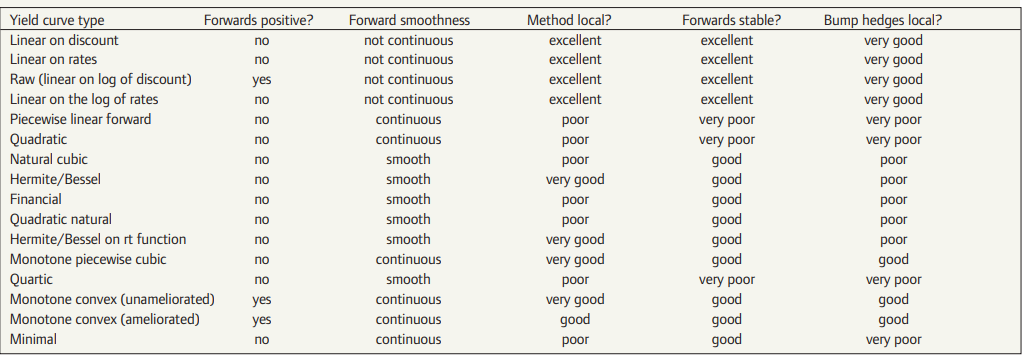
\includegraphics[width=1\textwidth]{Tables/InterpolationMethods.png}
        \caption{Interpolation Methods}
        \label{table:Interpolation_Methods}
    \end{table}
    
    \noindent
    Hagan and West \cite{hagan2008methods} highlight that the choice of interpolation scheme is critical not just for smoothness but also for preventing arbitrage opportunities. The structure of the forward rate curve  $f(t)$ is the primary visual and mathematical indicator of the quality of an interpolation method. This is because a negative forward rate implies that the discount factor function $Z(t)$ is not monotonically decreasing, which allows for arbitrage opportunities \cite{hagan2008methods}.

    \noindent
    Given this segmentation, the construction of the continuous discount curve $P(t,T)$ proceeds via a recursive algorithm that solves for discount factors sequentially, moving from the shortest maturities to the longest. Let $t$ denote the valuation (reference) date. The market provides a set of quoted instruments (deposits, FRAs, swaps) with strictly increasing terminal dates $\{d_i\}_{i=1}^n$, called \emph{calibration dates}. Each instrument contributes one pricing equation whose unknown is the discount factor $P(t,d_i)$. 
    
    \begin{itemize}
        \item Step 1: Initialization set $P(0,0) =1$
        \item Step 2: The curve is extended using deposits and FRAs. For the first instruments (typically up to 1 year), calculate $P(0,T_i)$ directly from the forward rate $F(0,T_{i-1},T_i)$
        \begin{equation} \label{eq:fraDF}
            P(0,T_i) = \frac{P(0,T_{i-1})}{1+F(0,T_{i-1},T_{i})\tau(T_{i-1},T_i)}
        \end{equation}
        \item Step 3: Assume the discount curve has been constructed up to time $T_{k-1}$.
        To solve for the discount factor at $T_k$ using a par swap with fixed rate $S_k$, we use the par swap equation. In a single-curve framework, the present value of the floating leg equals $1 - P(0,T_k)$ (under the standard no-notional-exchange logic). Equating floating and fixed legs gives
        \begin{equation}\label{eq:swap-core}
          1 - P(0,T_k)
          \;=\;
          S_k \sum_{i=1}^{k} \tau_i \, P(0,T_i),
        \end{equation}
        where $\alpha_i$ are the accrual fractions for the fixed-leg payments. Since $P(0,T_1),\dots,P(0,T_{k-1})$ are known from previous steps, we isolate $P(0,T_k)$ from \eqref{eq:swap-core}. If the swap includes intermediate payment dates $T_j$ with $T_{k-1} < T_j < T_k$ for which discount factors are not yet explicitly solved, we express these as functions of the known curve and the unknown target $P(0,T_k)$ via the chosen interpolation operator $\varphi$:
        \begin{equation}\label{eq:interp}
          P(0,T_j) \;=\; \varphi\!\big( T_j;\, \{(T_i,P(0,T_i))\}_{i=0}^{k-1},\, P(0,T_k) \big),
          \qquad T_{k-1} < T_j < T_k.
        \end{equation}
        Substituting \eqref{eq:interp} into \eqref{eq:swap-core} yields a (generally) nonlinear equation in the single unknown $P(0,T_k)$, which is then solved numerically. In the common case where all payment dates are on the existing grid (i.e., no intermediate unknowns), \eqref{eq:swap-core} reduces to a linear equation with the closed-form solution
        \begin{equation}\label{eq:swap-closed-form}
          P(0,T_k)
          \;=\;
          \frac{\,1 \;-\; S_k \displaystyle\sum_{i=1}^{k-1} \alpha_i P(0,T_i)\,}
               {\,1 + S_k \alpha_k\,}.
        \end{equation}
        \noindent 
        Repeat the recursive step for successive maturities until the longest instrument is exactly repriced, yielding a complete term structure $T \mapsto P(0,T)$. Between calibration dates, obtain a continuous curve using the selected interpolation method (e.g., linear in $\ln P(0,t)$, monotone convex).
    \end{itemize}

    \noindent
    The yield curve and the discount curve obtained from bootstrapping carry the same term-structure information but in different representations. The bootstrap algorithm produces discount factors $P(t,T)$, which are the fundamental inputs for pricing. The yield curve $R(t,T)$ is simply an alternative representation of the same term-structure information, obtained by converting discount factors into annualised zero rates under a chosen compounding convention.
    \begin{definition}[Yield Curve]\label{def:yield_curve}
    The \textbf{Yield Curve} at time \( t \) is the graph of the function:
    \begin{equation}
        T \mapsto R(t,T) \quad \text{for } T \geq t.
    \end{equation} 

    \end{definition}
    \noindent
    Practitioners pay attention to the shape of the yield curve: 
    \begin{itemize}
        \item \textbf{Upward-sloping (normal) yield curve:} Long-term yields exceed short-term yields, typically reflecting expectations of future economic growth, rising interest rates, and compensation for maturity and inflation risk.

        \item \textbf{Flat yield curve:} Short- and long-term yields are broadly similar, usually indicating a transition phase in the economy or uncertainty about future monetary policy, often preceding turning points in the interest rate cycle.
        
        \item \textbf{Inverted yield curve:} Short-term yields exceed long-term yields, commonly interpreted as a signal of expected economic slowdown or recession, as markets anticipate falling future interest rates.

        \item \textbf{Humped yield curve:} Medium-term yields exceed both short-term and long-term yields, producing a hump in the curve. This shape typically arises when markets anticipate near-term interest rate increases followed by a longer-term decline, or during periods of elevated uncertainty about the medium-term economic outlook. 
    \end{itemize}

    \begin{figure}[h!]
        \centering
        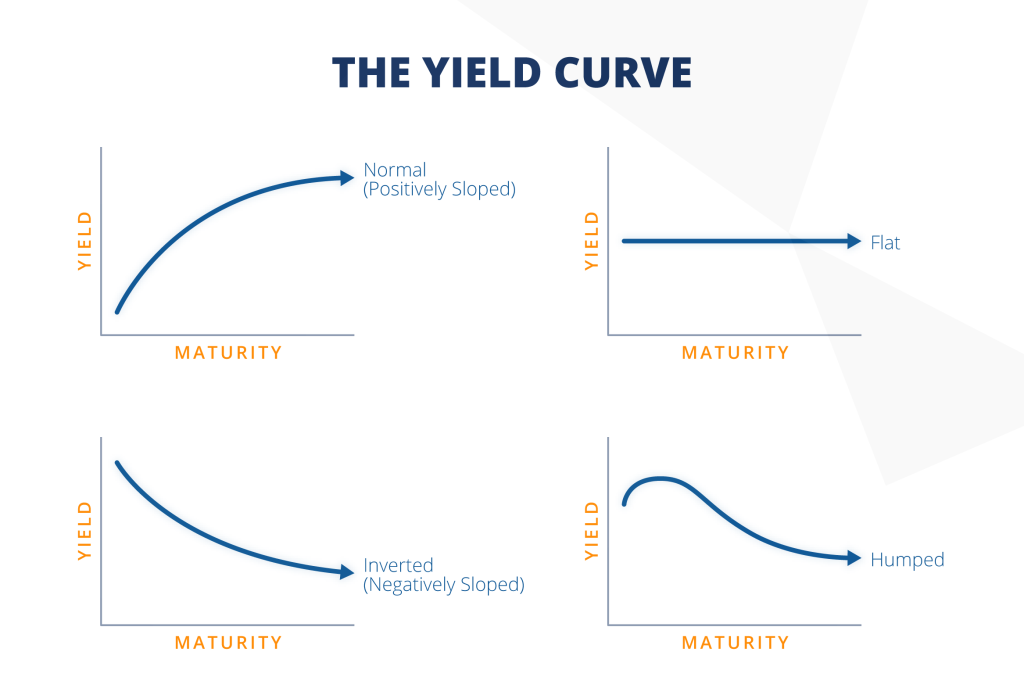
\includegraphics[width=0.9\textwidth]{Images/yield_curves_shapes.png}
        \caption{Typical yield curve shapes: upward-sloping (normal), flat, and inverted.}
        \label{fig:yield_curve_shapes}
    \end{figure}

    \subsection*{Parametric Curve Estimation: The Svensson Model}

    \noindent
    The bootstrapping algorithm above produces discount factors that exactly reprice all calibration instruments, but the resulting curve is piecewise in structure and sensitive to the choice of interpolation scheme. For applications requiring a globally smooth and differentiable term structure, an alternative approach is to fit a parametric functional form directly to observed market rates. Parametric models sacrifice exact repricing in favour of parsimony and smoothness, and are widely used by central banks for monetary policy analysis and for constructing initial term structures that serve as inputs to short-rate models \cite{bis2005zerocoupon}. The most widely adopted specification is the Svensson (1994) extension of the Nelson-Siegel model, which decomposes the instantaneous forward curve into four factor loadings and two decay parameters \cite{svensson1994estimating}.

    \noindent
    The Svensson model specifies the instantaneous forward rate $f(0,t)$ as:
    \begin{equation}\label{eq:svensson-forward}
        f(0,t) = \beta_0 + \beta_1 e^{-t/\tau_1}
                + \beta_2 \frac{t}{\tau_1} e^{-t/\tau_1}
                + \beta_3 \frac{t}{\tau_2} e^{-t/\tau_2}
    \end{equation}
    Integrating over $[0,t]$ and dividing by $t$ yields the corresponding continuously compounded zero rate:
    \begin{equation}\label{eq:svensson-zero}
        R(0,t) = \beta_0
                + \beta_1 \frac{1-e^{-t/\tau_1}}{t/\tau_1}
                + \beta_2 \left(\frac{1-e^{-t/\tau_1}}{t/\tau_1} - e^{-t/\tau_1}\right)
                + \beta_3 \left(\frac{1-e^{-t/\tau_2}}{t/\tau_2} - e^{-t/\tau_2}\right)
    \end{equation}
    The six parameters carry direct economic interpretations:
    \begin{itemize}
        \item $\beta_0 > 0$: the long-run level of interest rates, to which the curve converges as $t \to \infty$
        \item $\beta_1$: the slope factor, determining the spread between short- and long-term rates; a negative value produces an upward-sloping curve
        \item $\beta_2$: the first curvature factor, generating a hump or trough that peaks near maturity $\tau_1$
        \item $\beta_3$: the second curvature factor, allowing an additional hump near maturity $\tau_2$, extending the flexibility of the original Nelson-Siegel specification
        \item $\tau_1, \tau_2 > 0$: decay parameters controlling how quickly the slope and curvature contributions revert to zero with increasing maturity
    \end{itemize}
    The parameters are estimated by minimising the sum of squared deviations between model-implied and observed market zero rates across calibration maturities \cite{svensson1994estimating}:
    \begin{equation}\label{eq:svensson-calib}
        \min_{\beta_0,\,\beta_1,\,\beta_2,\,\beta_3,\,\tau_1,\,\tau_2}
        \sum_{i} \left(R^{\mathrm{market}}(0,t_i) - R(0,t_i)\right)^2
    \end{equation}

    \noindent
    The Svensson model is of particular relevance to the Hull-White framework developed in this study. Calibrating the time-dependent drift $\theta(t)$ to the initial term structure requires evaluating $\partial f(0,t)/\partial t$, since the exact expression for $\theta(t)$ depends on the slope of the initial forward curve at every point in time. A piecewise bootstrapped curve, being discontinuous between calibration pillars, yields an unreliable numerical derivative at those points. The Svensson forward rate in Equation~\eqref{eq:svensson-forward} is smooth and analytically differentiable everywhere, supplying a stable and consistent input to the Hull-White calibration described in the methodology chapter.

    \subsection*{HJM Framework}
    \noindent
    The evolution of term structure modelling represents a structural shift in how interest rate models are formulated. Early equilibrium models, such as Vasicek (1977) and Cox-Ingersoll-Ross (1985), specified the dynamics of the instantaneous short rate $r(t)$ under a risk-neutral measure and derived the yield curve as an output \cite{Green_2016}. This endogenous approach had a fundamental practical deficiency: because the initial yield curve was a model output rather than an input, these models could not exactly reprice the liquid benchmark instruments observed in the market, introducing systematic pricing errors that undermined their use in derivative valuation \cite{oosterlee2019mathematical}. The HJM framework addressed this by reversing the modelling direction entirely. \\

    \noindent
    Before stating the HJM dynamics, we formalise the object being modelled. The term structure of interest rates is not a single scalar but a continuum of rates indexed by maturity, admitting three equivalent representations.

    \begin{definition}[Term Structure]\label{def:term_structure}
    The \textbf{term structure of interest rates} at time $t$ is the collection of discount factors $\{P(t,T) : T \geq t\}$, or equivalently the family of mappings
    \begin{equation}
        T \mapsto R(t,T), \qquad T \mapsto f(t,T), \qquad T \mapsto P(t,T), \quad T \geq t,
    \end{equation}
    where $R(t,T)$ is the continuously compounded zero rate, $f(t,T)$ is the instantaneous forward rate, and $P(t,T)$ is the zero-coupon bond price. Each representation encodes the same term-structure information and must be consistent with observed market prices and the no-arbitrage conditions of Theorems~\ref{thm:FTAP} and~\ref{thm:SFTAP}.
    \end{definition}

    \noindent
    Given any one of the three representations, the other two are recovered without loss of information. The zero-coupon bond price $P(t,T)$ is the most fundamental, since it is the discounting kernel for future cash flows, but the instantaneous forward rate $f(t,T)$ is the most convenient state variable for modelling the dynamics of the entire curve, as it is directly observable in the limit of the simple compounded forward rate. \\

    \noindent
    The Heath-Jarrow-Morton (HJM) framework \cite{kwok2008mathematical} resolved the endogeneity problem by taking the initial forward rate curve $f(0,\cdot)$ as a given infinite-dimensional input, calibrated directly to market data, and specifying only the stochastic dynamics of its evolution through time. This ensures an automatic, exact fit to the observed term structure at $t = 0$. Within this framework, the Hull-White (1990) model emerges not merely as an extension of Vasicek but as a specific, Markovian restriction of the general HJM dynamics that retains analytic tractability while preventing arbitrage \cite{Green_2016}. \\

    \noindent
    Under the smoothness assumption on $P(t,T)$ in Definition~\ref{def:zcb}, the instantaneous forward rate is well-defined for all $T \geq t$ and is related to the simple compounded forward rate $F(t,T,T+\Delta T)$ introduced in Definition~\ref{def:forward_rate} by taking the limit as the accrual period shrinks to zero \cite{brigo2001interest}.

    \begin{definition}[Instantaneous Forward Rate] \label{def:inst_forward_rate}
    The \textbf{instantaneous forward rate} $f(t,T)$ prevailing at time $t$ for maturity $T > t$ is defined by
    \begin{equation}
        f(t,T) = \lim_{\Delta T \to 0} F(t,T,T+\Delta T) = -\frac{\partial}{\partial T} \ln P(t,T)
    \end{equation}
    \end{definition}

    \noindent
    The zero-coupon bond price is recovered from the instantaneous forward rate by integration:
    \begin{equation}
        P(t,T) = \exp\!\left(-\int_t^T f(t,u)\,du\right)
    \end{equation}
    The instantaneous short rate $r(t)$ is the limiting case at the current time:
    \begin{equation}
        r(t) = f(t,t) = \lim_{T \downarrow t} R(t,T)
    \end{equation}
    These relationships confirm that the instantaneous forward curve $T \mapsto f(t,T)$ is a complete description of the term structure: it determines all bond prices and all spot rates simultaneously. \\

    \noindent
    The HJM framework models the stochastic evolution of the entire forward curve simultaneously. Under the risk-neutral measure $\mathbb{Q}$, the dynamics of $f(t,T)$ for all maturities $T \geq t$ are governed by the SDE
    \begin{equation}
        df(t,T) = \alpha(t,T)\,dt + \sigma(t,T)\,dW(t)
    \end{equation}
    where $W(t)$ is a standard Brownian motion under $\mathbb{Q}$ and $\sigma(t,T)$ is the volatility structure. The central contribution of Heath, Jarrow, and Morton is that, under the risk-neutral measure, the drift $\alpha(t,T)$ is not a free modelling choice but is uniquely determined by the volatility structure through the no-arbitrage drift condition. For a one-factor model,
    \begin{equation}
        \alpha(t,T) = \sigma(t,T)\int_t^T \sigma(t,u)\,du
    \end{equation}
    This result means the modeller specifies only $\sigma(t,T)$ and the initial curve $f(0,T)$; the no-arbitrage requirement then determines the entire future evolution of the term structure \cite{kwok2008mathematical}. However, for a general choice of $\sigma(t,T)$, the HJM dynamics are non-Markovian: the state of the forward curve at time $t$ depends on the full path of $W$, not merely on its current value. In a lattice implementation, this produces non-recombining trees whose node count grows exponentially with the number of time steps, rendering the general framework computationally intractable for large derivative portfolios \cite{Green_2016, Hull_2018}.

    \noindent
    The Hull-White model resolves this by imposing an economically motivated constraint on the volatility structure \cite{Hull_2018}. If $\sigma(t,T)$ is chosen to be exponentially decaying in the time-to-maturity $(T-t)$,
    \begin{equation}
        \sigma(t,T) = \sigma\,e^{-a(T-t)}
    \end{equation}
    then the HJM dynamics collapse to a Markovian system driven by the single state variable $r(t)$ \cite{kwok2008mathematical}. This volatility structure has a direct economic interpretation: shocks to the short end of the forward curve dampen at rate $a$ as maturity increases, encoding mean reversion directly into the curve dynamics \cite{gupta2005pricing}. Under this specification, the short rate follows the SDE
    \begin{equation}
        dr(t) = [\theta(t) - a\,r(t)]\,dt + \sigma\,dW(t)
    \end{equation}
    where $a > 0$ is the mean reversion speed, $\sigma > 0$ is the instantaneous volatility, and $\theta(t)$ is a deterministic function calibrated to fit the initial term structure exactly. This calibration requires the initial instantaneous forward curve and its time derivative, which the Svensson parametrisation introduced above supplies analytically \cite{brigo2001interest}:
    \begin{equation}\label{eq:theta}
        \theta(t) = \frac{\partial f^M(0,t)}{\partial t} + a\,f^M(0,t)
                  + \frac{\sigma^2}{2a}\!\left(1 - e^{-2at}\right)
    \end{equation}
    where $f^M(0,t)$ denotes the market-implied initial instantaneous forward rate. This formulation reduces the entire state of the term structure to the single variable $r(t)$, permitting efficient simulation via recombining trinomial trees and Monte Carlo methods. \\

    \noindent
    Since the Hull-White SDE is linear in $r(t)$, it admits an exact closed-form solution requiring no approximation, a property that sets it apart from nonlinear short-rate models such as Cox-Ingersoll-Ross, where explicit solutions do not exist in general \cite{brigo2001interest}. The standard technique is to multiply both sides of the SDE by the integrating factor $e^{at}$, which converts the left-hand side into a perfect differential via It\^{o}'s product rule:
    \begin{equation}
        d\!\left(e^{at}r(t)\right) = e^{at}\theta(t)\,dt + \sigma e^{at}\,dW(t)
    \end{equation}
    Integrating both sides from $s$ to $t$ and dividing through by $e^{at}$ yields the explicit solution:
    \begin{equation}\label{eq:hw-solution}
        r(t) = e^{-a(t-s)}r(s) + \int_s^t e^{-a(t-u)}\theta(u)\,du
               + \sigma\int_s^t e^{-a(t-u)}\,dW(u)
    \end{equation}

    \noindent
    The solution decomposes the short rate into three additive components, each with a clear economic interpretation. The first term, $e^{-a(t-s)}r(s)$, is the mean-reverting decay of the current short rate: the factor $e^{-a(t-s)}$ pulls the current value exponentially towards zero at rate $a$, so that the influence of today's rate diminishes as the horizon lengthens. The second term is the accumulated contribution of the deterministic drift $\theta(u)$, weighted by the same exponential decay, representing the path along which the expected short rate is continuously attracted towards the market-implied forward curve. The third term is the stochastic component: a weighted sum of Brownian increments $dW(u)$ accumulated from $s$ to $t$, with older shocks discounted more heavily than recent ones. In plain terms, the short rate at any future time is the net result of where it starts, where the market implies it is heading, and the random disturbances that arrive along the way \cite{Hull_2018}. \\

    \noindent
    Because the stochastic integral in Equation~\eqref{eq:hw-solution} is a linear functional of Brownian motion, it is Gaussian by construction. This means that, conditional on the filtration $\mathcal{F}_s$, the short rate $r(t)$ is normally distributed \cite{brigo2001interest}:
    \begin{equation}\label{eq:hw-dist}
        r(t)\,|\,\mathcal{F}_s \;\sim\; \mathcal{N}\!\left(\mu(s,t),\; V(s,t)\right)
    \end{equation}
    with conditional mean and variance:
    \begin{equation}\label{eq:hw-mean}
        \mu(s,t) = e^{-a(t-s)}r(s) + \int_s^t e^{-a(t-u)}\theta(u)\,du
    \end{equation}
    \begin{equation}\label{eq:hw-var}
        V(s,t) = \frac{\sigma^2}{2a}\!\left(1 - e^{-2a(t-s)}\right)
    \end{equation}
    The mean $\mu(s,t)$ reflects the two deterministic forces already identified in the explicit solution: the decayed current rate and the forward-curve-implied drift. The variance $V(s,t)$ increases monotonically from zero at $t = s$ and saturates at $\sigma^2/(2a)$ as $t \to \infty$. This saturation is a direct consequence of mean reversion: unlike a driftless Brownian motion, where uncertainty accumulates without bound, mean reversion prevents the short rate from wandering arbitrarily far from the forward curve, bounding the long-run uncertainty by the ratio of volatility to mean reversion speed \cite{kwok2008mathematical}. \\

    \noindent
    The Gaussian structure of the solution has three direct consequences for this study. First, since bond prices take the form $P(t,T) = A(t,T)\,e^{-B(t,T)r(t)}$ and $r(t)$ is normally distributed, bond prices are lognormally distributed. This is precisely the property that enables the closed-form ATSM expressions derived below and underpins the analytical swaption and cap pricing formulae used for calibrating $a$ and $\sigma$ to market data \cite{brigo2001interest}. \\

    \noindent
    Second, the normal distribution assigns positive probability to negative values of $r(t)$ for all $t > s$. Negative short rates are inconsistent with the classical interpretation of the money market account as a locally riskless investment accumulating at the prevailing short rate, and represent a theoretical limitation of the Gaussian specification \cite{Green_2016}. In practice, the probability of negative rates under calibrated Hull-White parameters is small for typical upward-sloping or flat term structures, and the analytical tractability of the Gaussian model is considered to outweigh this limitation for the IRS portfolio considered in this study. \\

    \noindent
    Third, and most directly relevant to the numerical methodology, the exact conditional distribution in Equation~\eqref{eq:hw-dist} means that Monte Carlo simulation of the short rate requires no time-stepping approximation. At each simulation step $[t_i, t_{i+1}]$ with $\Delta t = t_{i+1} - t_i$, the short rate is drawn exactly from its conditional distribution \cite{brigo2001interest}:
    \begin{equation}\label{eq:hw-mc}
        r(t_{i+1}) = e^{-a\Delta t}r(t_i) + \mu_{\Delta}(t_i)
                   + \sqrt{V(t_i,\,t_{i+1})}\;Z_i,
                   \quad Z_i \overset{\text{iid}}{\sim} \mathcal{N}(0,1)
    \end{equation}
    where $\mu_{\Delta}(t_i) = \int_{t_i}^{t_{i+1}} e^{-a(t_{i+1}-u)}\theta(u)\,du$ is the deterministic drift contribution over the step. Unlike the Euler-Maruyama scheme, which introduces a strong-order bias proportional to $\Delta t$, this discretisation is exact: the only source of error in the simulated short rate paths is Monte Carlo sampling variance, which diminishes at the standard $1/\sqrt{N}$ rate as the number of simulated paths $N$ increases \cite{kwok2008mathematical}. This exact simulation scheme is used directly in the exposure and xVA calculations of the methodology chapter. \\

    \noindent
    A further analytical advantage of the Hull-White model is its classification as an Affine Term Structure Model (ATSM), which yields closed-form zero-coupon bond prices. Given $r(t)$, the time-$t$ price of a zero-coupon bond maturing at $T$ takes the exponential affine form
    \begin{equation}
        P(t,T) = A(t,T)\,\mathrm{e}^{-B(t,T)\,r(t)}
    \end{equation}
    where the deterministic functions $B(t,T)$ and $A(t,T)$ are given by \cite{brigo2001interest}
    \begin{equation}\label{eq:hw-B}
        B(t,T) = \frac{1 - e^{-a(T-t)}}{a}
    \end{equation}
    \begin{equation}\label{eq:hw-lnA}
        \ln A(t,T) = \ln\frac{P^M(0,T)}{P^M(0,t)} - B(t,T)\,f^M(0,t)
                   - \frac{\sigma^2}{4a}\!\left(1 - e^{-2at}\right)B(t,T)^2
    \end{equation}
    The affine structure admits closed-form expressions for European swaptions and caps, making model calibration tractable: the parameters $a$ and $\sigma$ are typically estimated by fitting to the ``diagonal'' of the swaption volatility matrix or a strip of at-the-money cap volatilities \cite{brigo2001interest}. The principal limitation of the one-factor specification is that all instantaneous forward rates are driven by a single Brownian motion, implying perfect instantaneous correlation across the curve. This precludes exact replication of portfolios sensitive to non-parallel yield curve movements such as twists and butterflies, a limitation acknowledged in the calibration discussion of the following chapter.

    \chapter{Counterparty Credit Risk and xVAs}

    \noindent
    The post-crisis derivatives market fundamentally altered the way in which banks price and manage OTC derivatives. Prior to 2008, the prevailing assumption in quantitative finance was that counterparties to a derivative transaction were effectively default-free, allowing the standard risk-neutral price to serve as a complete valuation \cite{Green_2016}. The collapse of Lehman Brothers in September 2008 made explicit what had previously been treated as negligible: every OTC derivative trade carries bilateral exposure to counterparty default, and that exposure carries an economic cost that must be reflected in the price \cite{Gregory_2015}. This chapter formalises the mathematical framework underlying that cost. Section~\ref{sec:ccr} defines the exposure measures central to counterparty risk quantification. Section~\ref{sec:credit-mitigants} introduces the legal and contractual mechanisms that reduce but do not eliminate counterparty exposure. Section~\ref{sec:cva-dva} derives the Credit Valuation Adjustment (CVA) and Debit Valuation Adjustment (DVA) as expectation integrals over simulated exposure profiles. These integrals are evaluated numerically in Chapter~7 using the Hull-White Monte Carlo engine introduced in Chapter~5.

    \section*{Counterparty Credit Risk}
    \label{sec:ccr}

    \noindent
    Counterparty credit risk (CCR) is the risk that a counterparty to a financial transaction will fail to fulfil its payment obligations before the final settlement of the trade \cite{Green_2016}. Unlike loan credit risk, where exposure is one-directional and fixed at inception, the exposure arising from a derivatives transaction is bilateral and dynamic: the direction of net exposure reverses as market rates evolve, and its magnitude can grow substantially over the life of a long-dated contract \cite{cesari2009modelling, Gregory_2015}. \\

    \noindent
    The central quantity in CCR measurement is the \textbf{exposure at default} (EAD), defined as the net amount owed by the defaulting counterparty at the instant of default. Since OTC derivatives can carry both positive and negative mark-to-market value, the EAD from the perspective of party $A$ is
    \begin{equation}
        \text{EAD}(t) = \max\!\left(V(t),\, 0\right),
        \label{eq:EAD}
    \end{equation}
    where $V(t)$ denotes the mark-to-market value of the netted derivative portfolio at time $t$ \cite{Gregory_2015}. When $V(t) < 0$, party $A$ owes the counterparty money and no credit exposure exists from $A$'s perspective at that instant. \\

    \noindent
    Since default can occur at any point during the tenor of the contract, CCR management requires a forward-looking view of the exposure profile. Two expectation-based measures are standard \cite{canabarro2003measuring, zhu2007guide}. The \textbf{expected positive exposure} (EPE) and \textbf{expected negative exposure} (ENE) at time $t$ are defined, respectively, as
    \begin{align}
        \text{EPE}(t) &= \mathbb{E}_t\!\left[\max\!\left(V(t),\, 0\right)\,\middle|\,\mathcal{F}_t\right], \label{eq:EPE} \\[4pt]
        \text{ENE}(t) &= \mathbb{E}_t\!\left[\max\!\left(-V(t),\, 0\right)\,\middle|\,\mathcal{F}_t\right]. \label{eq:ENE}
    \end{align}
    Both quantities are non-negative by construction. The EPE profile captures the average exposure of party $A$ to counterparty default, whilst the ENE profile captures the average exposure of the counterparty to party $A$'s own default. The EPE feeds directly into the CVA calculation and the ENE into the DVA calculation, as formalised in Section~\ref{sec:cva-dva}. \\

    \noindent
    In the event of default, the non-defaulting party does not lose the full EAD. A fraction of the outstanding claim, the \textbf{recovery rate} $R \in [0,1]$, is recovered through the bankruptcy process. The complementary quantity
    \begin{equation}
        \text{LGD} = 1 - R
        \label{eq:LGD}
    \end{equation}
    is the \textbf{loss given default}, the true economic loss per unit of exposure \cite{Green_2016}. In the bilateral setting of this study, separate recovery rates $R_C$ and $R_B$ are assigned to the counterparty and to the bank respectively, with corresponding losses given default $\text{LGD}_C = 1 - R_C$ and $\text{LGD}_B = 1 - R_B$. \\

    \noindent
    A further complication in CCR arises when the exposure is correlated with the creditworthiness of the defaulting party. \textbf{Wrong-way risk} occurs when the exposure to a counterparty increases precisely as the counterparty's credit quality deteriorates, amplifying the potential loss beyond what is implied by an unconditional EPE profile \cite{Green_2016}. For interest rate swaps, a corporate counterparty that pays fixed and receives floating may face financial stress in high-rate environments, exactly when the swap carries positive value to the bank. \textbf{Right-way risk} is the converse: a favourable correlation between exposure and credit quality reduces realised losses relative to the unconditional EPE \cite{Gregory_2015}. This study assumes independence between the short-rate process and the default intensities $\lambda_C$ and $\lambda_B$, setting aside wrong-way and right-way risk effects in order to isolate the contribution of the Hull-White interest rate model to the exposure profile.

    \section*{Credit Risk Mitigants}
    \label{sec:credit-mitigants}

    \noindent
    Several contractual arrangements exist to reduce counterparty credit exposure in the OTC derivatives market. \\

    \noindent
    \textbf{Close-out netting.} A close-out netting agreement, enshrined in the ISDA Master Agreement, provides the legal basis for offsetting positive and negative mark-to-market values across a portfolio of trades between two counterparties at the moment one party defaults \cite{Green_2016}. Without netting, the surviving party must honour trades with negative value whilst filing as an unsecured creditor for trades with positive value; under netting, only the net portfolio value constitutes the EAD. Research by ISDA suggests that netting can reduce aggregate credit exposure by as much as 85\% for diversified derivatives portfolios \cite{brigo2013counterparty}. \\

    \noindent
    \textbf{Collateral and the CSA.} A Credit Support Annex (CSA), attached to the ISDA Master Agreement, governs the periodic posting of collateral between counterparties in support of the mark-to-market of the portfolio. The call frequency, minimum transfer amount, eligible collateral types, and counterparty-specific thresholds are all specified contractually \cite{Green_2016}. A CSA does not eliminate credit exposure entirely: the residual exposure over the margin period of risk, the interval between the last collateral posting and the close-out of the position, generates a smaller but non-zero CVA even for collateralised trades. \\

    \noindent
    For the purposes of this study, we adopt the clean exposure assumption: no CSA is in place, and the full expected positive exposure profile is exposed to counterparty default. This is consistent with the bilateral, uncollateralised interest rate swap transactions that motivate the xVA calculations in Chapter~7, and it ensures that the computed CVA and DVA reflect the unmitigated bilateral credit adjustment.

    \section*{Credit and Debit Valuation Adjustments}
    \label{sec:cva-dva}

    \noindent
    The credit-risky value of a bilateral derivative differs from its default-free, risk-neutral counterpart whenever either counterparty faces a non-zero probability of default. Burgard and Kjaer \cite{pde_2011, burgard2011balance} derived the governing PDE for this bilateral credit-risky value via a replication argument under the risk-neutral measure, accounting separately for the cost of the counterparty's default through CVA and the benefit of the bank's own default through DVA.

    \begin{thmbox}{}{thm:credit-risky-pde}
        The price of a credit risky derivative trade satisfies the following PDE
        \[
        \left\{
        \begin{array}{l}
            \dfrac{\partial \hat{V}}{\partial t} + \mathcal{A}_t \hat{V} - r\hat{V} = \lambda_C(1-R_C)V^+ + \lambda_B(1-R_B)V^- \\[10pt]
            \hat{V}_T = V_T \text{ is the final payoff of the derivative}
        \end{array}
        \right.
        \]
        where the risk-free price satisfies the Black-Scholes PDE
        \[
        \left\{
        \begin{array}{l}
            \dfrac{\partial V}{\partial t} + \mathcal{A}_t V - rV = 0 \\[10pt]
            V_T \text{ is the final payoff of the derivative}
        \end{array}
        \right.
        \]
        and the parabolic differential operator is given by
        \[
            \mathcal{A}_t = \frac{1}{2}\sigma^2 S^2 \frac{\partial^2}{\partial S^2} + rS\frac{\partial}{\partial S}.
        \]
    \end{thmbox}

    \noindent
    In the bilateral PDE, $\hat{V}$ denotes the credit-risky derivative price, $V$ is the default-free risk-neutral price, $\lambda_C$ and $\lambda_B$ are the risk-neutral default intensities (hazard rates) of the counterparty and the bank, $R_C$ and $R_B$ are their respective recovery rates, and $V^+ = \max(V,0)$ and $V^- = \min(V,0)$ denote the positive and negative parts of the default-free price. The operator $\mathcal{A}_t$ is the infinitesimal generator of the underlying state process; for the Hull-White interest rate model considered in this study it takes the form $\mathcal{A}_t = [\theta(t) - ar]\,\partial_r + \tfrac{1}{2}\sigma^2\,\partial_{rr}$, whilst for an equity underlying it reduces to the Black-Scholes generator as written above. The structure of the bilateral PDE is unchanged across both settings. The right-hand side decomposes into two channels: the term $\lambda_C(1-R_C)V^+$ is the CVA source, which reduces the credit-risky price relative to the default-free price when the portfolio has positive value to the bank; and the term $\lambda_B(1-R_B)V^-$ is the DVA source, which increases the credit-risky price when the portfolio has negative value to the bank, since the bank's own default then constitutes a benefit to the surviving counterparty. \\

    \noindent
    Applying the Feynman-Kac theorem to the bilateral PDE and taking expectations under the risk-neutral measure $\mathbb{Q}$, the bilateral credit-risky price decomposes as \cite{pde_2011, brigo2013counterparty}
    \begin{equation}
        \hat{V}(t) = V(t) - \text{CVA}(t) + \text{DVA}(t).
        \label{eq:bilateral-price}
    \end{equation}
    The \textbf{Credit Valuation Adjustment} is the expected loss to the bank from the counterparty's default, weighted by the counterparty's default intensity:
    \begin{equation}
        \text{CVA}(t) = \text{LGD}_C \int_t^T \text{EPE}(s)\,\lambda_C(s)\,ds.
        \label{eq:CVA}
    \end{equation}
    The \textbf{Debit Valuation Adjustment} is the expected gain to the bank from its own default, weighted by the bank's default intensity:
    \begin{equation}
        \text{DVA}(t) = \text{LGD}_B \int_t^T \text{ENE}(s)\,\lambda_B(s)\,ds.
        \label{eq:DVA}
    \end{equation}
    CVA is always non-negative and reduces the bilateral price; DVA is always non-negative and increases it. The combined \textbf{bilateral credit valuation adjustment} (BCVA) is
    \begin{equation}
        \text{BCVA}(t) = \text{CVA}(t) - \text{DVA}(t),
        \label{eq:BCVA}
    \end{equation}
    so that $\hat{V}(t) = V(t) - \text{BCVA}(t)$. When $\text{BCVA} > 0$ the net credit adjustment reduces the trade value; when $\text{BCVA} < 0$ the DVA benefit dominates. The sign of BCVA depends on the relative default intensities and recovery rates of both parties and on the direction of the net exposure profile \cite{Green_2016, Gregory_2015}. \\

    \noindent
    The EPE and ENE integrals in equations~\eqref{eq:CVA} and~\eqref{eq:DVA} are not available in closed form for a general stochastic term structure. They are evaluated numerically in Chapter~7 by simulating the Hull-White short rate along Monte Carlo paths and computing the expected exposures at each simulation date using the closed-form IRS valuation established in Chapter~5.

    \chapter{Neural Networks and Deep Learning}

    The tractability of derivative pricing under classical models rests on analytical or semi-analytical solutions that are available only under restrictive assumptions. Under the xVA framework developed in the preceding chapter, pricing must be performed across thousands of Monte Carlo simulation paths for the purpose of computing exposure profiles, and the computational cost of re-pricing a full derivatives portfolio at each time step is severe. Neural networks offer a principled response to this challenge, a trained network can emulate the pricing function to high accuracy whilst evaluating at a fraction of the computational cost of the underlying model. This chapter develops the mathematical foundations of neural networks and deep learning that underpin the surrogate modelling methodology employed in this study.

    \section*{The Artificial Neuron}

    The artificial neuron is the atomic computational unit of a neural network. Inspired by the threshold-activation behaviour of biological neurons, the artificial neuron receives a vector of inputs $\mathbf{x} = (x_1, \ldots, x_m)^{\top}$, computes a weighted sum, and produces an output determined by whether that sum exceeds a threshold. Given weights $w_1, \ldots, w_m$ and threshold $\theta$, the neuron activates if

    \[
    h = \sum_{i=1}^{m} w_i x_i > \theta.
    \]

    \noindent 
    Reparameterising by absorbing the threshold as a bias $b = -\theta$, the activation condition becomes $\sum_{i=1}^{m} w_i x_i + b > 0$. The boundary $\sum_{i=1}^{m} w_i x_i + b = 0$ defines a hyperplane in $\mathbb{R}^m$, and the
    neuron partitions its input space into two half-spaces. This constitutes the linear discriminant, and it represents the simplest possible classifier \citep{goodfellow2016deep}. \\

    \noindent
    The perceptron learning rule adjusts weights in response to classification errors. Given input $\mathbf{x}$, target $t \in \{0, 1\}$, and current output $y \in \{0, 1\}$, the update is

    \[
    w_i \leftarrow w_i + \eta(t - y)\, x_i, \qquad b \leftarrow b + \eta(t - y),
    \]

    \noindent 
    where $\eta \in (0, 1)$ is the learning rate, a scalar controlling the magnitude of each correction. When the prediction is correct ($t = y$), no update occurs. When the neuron fires incorrectly, the weight vector is adjusted in the direction of $\mathbf{x}$ (or its negative), geometrically moving the separating hyperplane toward the misclassified point. The algorithm converges in finite time when the dataset is linearly separable \citep{goodfellow2016deep}. When it is not, a single neuron is insufficient: the mapping from inputs to outputs cannot be represented as a single linear discriminant, and a richer architecture is required. \\

    \section*{Multi-Layer Perceptrons}

    The limitation of the single-layer perceptron motivates the multi-layer perceptron (MLP). The XOR function illustrates the issue directly: no single hyperplane separates its positive inputs $(0,1)$ and $(1,0)$ from its negative inputs $(0,0)$ and $(1,1)$, yet two hyperplanes suffice. The MLP achieves this by introducing hidden layers: each hidden layer learns an intermediate representation, and the output layer combines those representations to produce the network's decision or prediction \citep{rumelhart1986learning}. \\


    \noindent
    An MLP with $L$ layers is specified as follows. The input layer carries the raw features $\mathbf{x} \in \mathbb{R}^{d_0}$. Each subsequent layer $k = 1, \ldots, L$ receives the activation vector $\mathbf{a}_{k-1}$ from the preceding layer, applies a weight matrix $W_k \in \mathbb{R}^{d_{k-1} \times d_k}$ and a bias vector $\mathbf{b}_k \in \mathbb{R}^{d_k}$, and passes the result through an activation function $g_k$:

    \[
    \mathbf{a}_k = g_k\!\left(\mathbf{a}_{k-1} W_k + \mathbf{b}_k\right).
    \]

    \noindent
    The output layer produces $\mathbf{y} = \mathbf{a}_L$. The collection of all weights and biases across layers is denoted $\mathbf{W}$, and training amounts to finding the values of $\mathbf{W}$ that minimise a chosen measure of prediction error on the training data.

    \begin{figure}[htbp]
    \centering
    \begin{tikzpicture}[
        neuron/.style={circle, draw=blue!60!black, fill=blue!8,
                       minimum size=0.72cm, inner sep=0pt, line width=0.6pt},
        conn/.style={-Stealth, gray!50, line width=0.35pt},
        lbl/.style={font=\small},
        dim/.style={font=\footnotesize\itshape, text=blue!60!black},
        >=Stealth
    ]
    % Input layer
    \foreach \i/\y in {1/1.2, 2/0.0, 3/-1.2}
        \node[neuron] (I\i) at (0, \y) {};
    % Hidden layer 1
    \foreach \i/\y in {1/1.8, 2/0.6, 3/-0.6, 4/-1.8}
        \node[neuron] (H1\i) at (3.0, \y) {};
    % Hidden layer 2
    \foreach \i/\y in {1/1.8, 2/0.6, 3/-0.6, 4/-1.8}
        \node[neuron] (H2\i) at (6.0, \y) {};
    % Output layer
    \node[neuron] (O) at (9.0, 0.0) {};
    % Connections
    \foreach \i in {1,2,3}
        \foreach \j in {1,2,3,4}
            \draw[conn] (I\i) -- (H1\j);
    \foreach \i in {1,2,3,4}
        \foreach \j in {1,2,3,4}
            \draw[conn] (H1\i) -- (H2\j);
    \foreach \i in {1,2,3,4}
        \draw[conn] (H2\i) -- (O);
    % Layer labels
    \node[lbl, above=0.55cm] at (0.0, 1.2) {Input};
    \node[lbl, above=0.55cm] at (3.0, 1.8) {Hidden};
    \node[lbl, above=0.55cm] at (6.0, 1.8) {Hidden};
    \node[lbl, above=0.55cm] at (9.0, 0.7) {Output};
    % Dimension labels
    \node[dim, below=0.5cm] at (0.0, -1.2) {$d_0$};
    \node[dim, below=0.5cm] at (3.0, -1.8) {$d_1$};
    \node[dim, below=0.5cm] at (6.0, -1.8) {$d_2$};
    \node[dim, below=0.5cm] at (9.0, -0.7) {$d_L$};
    % Weight matrix labels
    \node[font=\footnotesize, text=gray!65] at (1.5, 2.2) {$W_1$};
    \node[font=\footnotesize, text=gray!65] at (4.5, 2.2) {$W_2$};
    \node[font=\footnotesize, text=gray!65] at (7.5, 1.4) {$W_L$};
    \end{tikzpicture}
    \caption{A feedforward MLP with $L = 3$ layers. Each node applies an activation
    function to a weighted sum of the preceding layer's outputs. Weight matrices
    $W_k \in \mathbb{R}^{d_{k-1} \times d_k}$ connect adjacent layers; the layer
    widths $d_0, \ldots, d_L$ are illustrative.}
    \label{fig:mlp_architecture}
    \end{figure}

    \section*{Activation Functions}

    The activation function $g_k$ introduces the non-linearity that gives multi-layer networks their expressive power. Without it, a composition of affine transformations collapses to a single affine transformation regardless of depth, and the MLP reduces to a linear model. The choice of activation function affects both the expressiveness of the network and the stability of training. \\

    \begin{itemize}
    \item \textbf{Sigmoid.} The logistic sigmoid $\sigma(z) = (1 + e^{-z})^{-1}$ maps $\mathbb{R}$ into $(0, 1)$ and is differentiable everywhere. Its derivative satisfies $\sigma'(z) = \sigma(z)(1 - \sigma(z))$, a self-referential identity that simplifies gradient computation considerably. The sigmoid saturates for large $|z|$, causing gradients to vanish in deep networks and impeding learning.

    \item \textbf{Hyperbolic tangent.} The function $\tanh(z) = (e^z - e^{-z})/(e^z + e^{-z})$ maps $\mathbb{R}$ into $(-1, 1)$ and is zero-centred, which tends to produce better-conditioned gradient flow than the sigmoid. Its derivative is $\tanh'(z) = 1 - \tanh^2(z)$. Like the sigmoid, tanh saturates at large magnitudes.

    \item \textbf{Rectified linear unit (ReLU).} The activation $\mathrm{relu}(z) = \max(0, z)$ is piecewise linear with derivative 1 for $z > 0$ and 0 for $z < 0$ \citep{glorot2011deep}. It does not saturate on the positive half-line, which mitigates the vanishing gradient problem and enables effective training of deep architectures. The sub-gradient at $z = 0$ is set to 0 by convention. ReLU is the standard choice for hidden layers in modern deep learning.

    \item \textbf{Linear.} The identity $\mathrm{lin}(z) = z$ is appropriate at the output layer of a regression network, where the target is a real-valued quantity such as a derivative price and no bounding of the output is required. Using a linear output activation ensures the network can produce outputs of arbitrary magnitude and sign.
    \end{itemize}

    \noindent
    The choice of output activation is determined by the task structure. For derivative pricing, where the target is a real-valued price, a linear output activation is standard \citep{ruf2020neural}. For binary classification, a sigmoid output is appropriate, for multi-class outputs, the softmax function $\mathrm{softmax}(z_{n_i}) = e^{z_{n_i}} / \sum_{j} e^{z_{n_j}}$ maps the pre-activations to a valid probability distribution over classes.

    \section*{The Universal Approximation Theorem}

    The theoretical justification for using neural networks as surrogate pricing functions is provided by the Universal Approximation Theorem. The result was established independently by \citet{cybenko1989approximation} for sigmoid activations and generalised to a broad class of activation functions by \citet{hornik1989multilayer, hornik1991approximation}.

    \begin{theorem}[Universal Approximation]
    \label{thm:uat}
    Let $g: \mathbb{R} \to \mathbb{R}$ be a continuous, bounded, and non-constant function. For any continuous function $f: K \to \mathbb{R}$ defined on a compact set $K \subset \mathbb{R}^d$ and any $\varepsilon > 0$, there exists a
    single-hidden-layer neural network $F_\varepsilon$ with activation $g$ such that
    \[
    \sup_{\mathbf{x} \in K} |F_\varepsilon(\mathbf{x}) - f(\mathbf{x})| < \varepsilon.
    \]
    \end{theorem}

    \noindent
    The theorem guarantees that a sufficiently wide single-hidden-layer network can approximate any continuous function to arbitrary precision on a compact domain. It is the composition of non-linear activations, rather than any specific sigmoid form, that confers this universal approximating capacity \citep{hornik1991approximation}. \\

    \noindent
    Three qualifications are essential. First, the theorem establishes existence but not constructibility: it provides no guidance on the network width required or on whether a particular training procedure will locate the approximating parameter configuration. Second, the result applies to compact domains; pricing functions defined over unbounded parameter ranges require additional regularity arguments. Third, approximation in theory does not imply generalisation in practice. A network may fit training inputs arbitrarily well whilst performing poorly on out-of-sample scenarios. The practical question of generalisation is addressed by training methodology and regularisation, treated in subsequent sections. \\

    \noindent
    In the context of this study, Theorem~\ref{thm:uat} justifies using a neural network to emulate the Hull-White pricing function $V(r, t; \boldsymbol{\theta})$, where $\boldsymbol{\theta}$ denotes the vector of model and trade parameters. Under standard regularity conditions, this function is continuous in its arguments, and the domain of interest can be taken as a compact hypercube in the space of short-rate scenarios \citep{mrad2025differential}.

    \section*{The Feedforward Pass}

    The feedforward pass computes the network output for a given input. For node $n$, the pre-activation is

    \[
    z_n = \sum_{m} w_{mn} y_m + b_n,
    \]

    \noindent
    where the sum ranges over all nodes $m$ in the preceding layer and $y_m$ is the post-activation output of node $m$. The post-activation of node $n$ is $y_n = g_n(z_n)$. Collecting across layers, the computation reduces to the
    sequential matrix propagation $\mathbf{a}_k = g_k(\mathbf{a}_{k-1} W_k + \mathbf{b}_k)$ evaluated from $k = 1$ to $k = L$. \\

    \noindent
    During the forward pass, the activation values $a_n = y_n|_{\mathbf{x}, \mathbf{W}}$ are stored for subsequent use in backpropagation. Storing these intermediate values is the mechanism by which the chain rule is applied efficiently without recomputation. \\

    \section*{Loss Functions}

    Training requires a scalar measure of the discrepancy between the network output $\mathbf{y}$ and the training target $\mathbf{t}$. This is the loss function $L(\mathbf{y}, \mathbf{t})$. \\

    \noindent 
    For regression tasks, the standard choice is the \textbf{mean squared error} (MSE), derived from the sum-of-squares loss:

    \[
    L(\mathbf{y}, \mathbf{t}) = \frac{1}{2} \sum_{j} (y_j - t_j)^2,
    \]

    \noindent 
    where the sum ranges over all output nodes $j$ \citep{goodfellow2016deep}. MSE penalises large deviations quadratically and is appropriate when the target is a continuous quantity and errors of larger magnitude are disproportionately costly. In the surrogate pricing context, the target is the derivative price and the loss is MSE over the training portfolio. \\

    \noindent 
    For multi-class classification tasks with a softmax output, the cross-entropy loss is preferred:

    \[
    L_{CE}(\mathbf{y}, \mathbf{t}) = -\sum_{i=1}^{k} t_i \ln(y_i),
    \]

    \noindent 
    where $\mathbf{t}$ is one-hot encoded and the softmax outputs form a probability distribution over classes \citep{goodfellow2016deep}. The softmax/cross-entropy pairing admits a particularly clean gradient: the output-layer delta simplifies to $\delta_n = a_n - t_n$, with no activation-derivative factor. This arises from the cancellation between the softmax Jacobian and the logarithmic derivative of the cross-entropy, and it makes the gradient at the output proportional to the raw prediction error. \\

    \section*{Backpropagation}

    Gradient descent minimises the loss by iteratively adjusting each parameter in the direction of steepest descent. The update rule for edge weight $w_{mn}$ is

    \[
    w_{mn} \leftarrow w_{mn} - \eta \frac{\partial L}{\partial w_{mn}}\bigg|_{\mathbf{x}, \mathbf{t}, \mathbf{W}}.
    \]

    \noindent 
    Computing these partial derivatives efficiently across all parameters of a multi-layer network is the purpose of the backpropagation algorithm \citep{rumelhart1986learning}. Backpropagation is a direct application of the
    multivariable chain rule: gradient information is propagated backward through the network from the output layer to the input layer, accumulating the partial derivatives of each node's contribution to the loss. \\

    \noindent 
    The central quantity is the \textbf{delta value} at node $n$:

    \[
    \delta_n = \frac{\partial L}{\partial z_n}\bigg|_{\mathbf{x}, \mathbf{t}, \mathbf{W}},
    \]

    \noindent 
    the partial derivative of the loss with respect to the pre-activation $z_n$ at the current weights and input. The weight gradient factorises as

    \[
    \frac{\partial L}{\partial w_{mn}}\bigg|_{\mathbf{x}, \mathbf{t}, \mathbf{W}} = \delta_n \cdot a_m,
    \]

    \noindent 
    so the weight update reduces to $w_{mn} \leftarrow w_{mn} - \eta \delta_n a_m$, and the bias update is $b_n \leftarrow b_n - \eta \delta_n$.

    \noindent 
    The backward pass computes delta values in two stages. At each output node $n$:

    \[
    \delta_n = (a_n - t_n) \cdot \frac{dy_n}{dz_n}\bigg|_\mathbf{W}.
    \]

    \noindent 
    For MSE loss with linear output activation, $dy_n/dz_n = 1$, giving $\delta_n = a_n - t_n$. For MSE loss with sigmoid output, $dy_n/dz_n = a_n(1 - a_n)$, giving $\delta_n = (a_n - t_n) a_n (1 - a_n)$. At each hidden node $n$, the delta is propagated from the succeeding layer:

    \[
    \delta_n = \left(\sum_{\ell} \delta_\ell \, w_{n\ell}\right) \cdot
    \frac{dy_n}{dz_n}\bigg|_\mathbf{W},
    \]

    \noindent 
    where $\ell$ ranges over all nodes in the layer immediately downstream of $n$, and $w_{n\ell}$ is the weight on the edge from $n$ to $\ell$. For ReLU hidden activations, $dy_n/dz_n = \mathbf{1}[z_n > 0]$; for tanh, $dy_n/dz_n = 1 - a_n^2$. The backward pass proceeds from the output layer to the first hidden layer. Once all delta values are available, all weights are updated. 

    \section*{Recurrent Neural Networks}

    The feedforward MLP processes each input independently, the output for a given input $\mathbf{x}$ is computed without reference to any prior inputs, and no information is carried across observations. This is appropriate when observations are exchangeable, but many problems in quantitative finance are inherently sequential. The short rate under Hull-White evolves as a continuous-time stochastic process, exposure profiles are indexed by a discrete time grid
    $0 = t_0 < t_1 < \cdots < t_K = T$; and xVA integrals accumulate contributions across simulation time steps. An architecture that maintains state across time is required to model such sequences. \\

    \noindent 
    The recurrent neural network (RNN) addresses this by introducing a hidden state $\mathbf{h}_t \in \mathbb{R}^d$ that is updated at each time step $t$ as a function of the current input $\mathbf{x}_t$ and the preceding hidden state $\mathbf{h}_{t-1}$ \citep{goodfellow2016deep}:

    \[
    \mathbf{h}_t = g\!\left(W_x\, \mathbf{x}_t + W_h\, \mathbf{h}_{t-1} + \mathbf{b}\right),
    \]

    \noindent 
    where $W_x \in \mathbb{R}^{n_x \times d}$ and $W_h \in \mathbb{R}^{d \times d}$ are learned weight matrices, $\mathbf{b} \in \mathbb{R}^d$ is a bias vector, and $g$ is an activation function, typically $\tanh$. The hidden state $\mathbf{h}_t$ serves as a compressed summary of the input history $\{\mathbf{x}_1, \ldots, \mathbf{x}_t\}$, and the output at time step $t$ is a function of $\mathbf{h}_t$. The same parameter matrices $W_x$, $W_h$, and $\mathbf{b}$ are shared across all time steps, this parameter sharing is what allows the network to process sequences of variable length and generalise across positions in the sequence. \\

    \noindent
    The RNN is trained by backpropagation through time (BPTT), the network is unrolled across $T$ time steps, producing a computational graph of depth $T$, and standard backpropagation is applied to this unrolled graph \citep{goodfellow2016deep}. The gradient of the loss with respect to the hidden state at time step $t$ involves a product of Jacobian matrices:

    \[
    \frac{\partial \mathbf{h}_t}{\partial \mathbf{h}_{t-k}}
    = \prod_{i=1}^{k} \frac{\partial \mathbf{h}_{t-i+1}}{\partial \mathbf{h}_{t-i}}
    = \prod_{i=1}^{k} \mathrm{diag}\!\left(g'(W_x \mathbf{x}_{t-i+1}
    + W_h \mathbf{h}_{t-i} + \mathbf{b})\right) W_h^{\top}.
    \]

    \noindent 
    If the spectral radius of $W_h$ is less than one, repeated multiplication causes this product to decay exponentially with $k$, effectively preventing the network from learning dependencies that span many time steps. If the spectral radius exceeds one, the product grows without bound and training becomes numerically unstable. These are the vanishing gradient and exploding gradient problems respectively, and they severely limit the practical usefulness of the basic RNN for long sequences \citep{hochreiter1997long}. Gradient clipping addresses the exploding case, but the vanishing problem requires a structural solution: gated architectures that create direct pathways for gradient flow across time. \\

    \begin{figure}[htbp]
    \centering
    \begin{tikzpicture}[
        cell/.style={draw=blue!60!black, fill=blue!8, rounded corners=5pt,
                     minimum width=1.6cm, minimum height=1.6cm,
                     font=\small\scshape, line width=0.8pt},
        arr/.style={-Stealth, line width=0.8pt},
        lbl/.style={font=\footnotesize},
        >=Stealth
    ]
    % RNN cells
    \node[cell] (C0) at (0.0, 0) {rnn};
    \node[cell] (C1) at (4.0, 0) {rnn};
    \node[cell] (C2) at (8.0, 0) {rnn};
    % Hidden state flow
    \draw[arr] (-2.2, 0) -- (C0.west)
        node[midway, above, lbl] {$\mathbf{h}_{t-2}$};
    \draw[arr] (C0.east) -- (C1.west)
        node[midway, above, lbl] {$\mathbf{h}_{t-1}$};
    \draw[arr] (C1.east) -- (C2.west)
        node[midway, above, lbl] {$\mathbf{h}_{t}$};
    \draw[arr] (C2.east) -- (10.2, 0)
        node[midway, above, lbl] {$\mathbf{h}_{t+1}$};
    % Inputs from below
    \foreach \x/\t in {0.0/{t-1}, 4.0/{t}, 8.0/{t+1}}
        \draw[arr] (\x, -2.0) -- (\x, -0.8)
            node[below=0.6cm, lbl] {$\mathbf{x}_{\t}$};
    % Outputs above
    \foreach \x/\t in {0.0/{t-1}, 4.0/{t}, 8.0/{t+1}}
        \draw[arr] (\x, 0.8) -- (\x, 2.0)
            node[above=0.0cm, lbl] {$\mathbf{y}_{\t}$};
    % Shared weights brace
    \draw[decorate,
          decoration={brace, amplitude=6pt, mirror, raise=4pt}]
        (-0.8, -1.8) -- (8.8, -1.8);
    \node[font=\footnotesize\itshape, text=blue!60!black] at (4.0, -2.7)
        {Shared parameters: $W_x,\; W_h,\; \mathbf{b}$};
    \end{tikzpicture}
    \caption{The RNN unrolled across three time steps. The recurrence
    $\mathbf{h}_t = g(W_x \mathbf{x}_t + W_h \mathbf{h}_{t-1} + \mathbf{b})$
    applies the same parameter matrices at every step. Training by BPTT requires
    propagating gradients through the full unrolled graph; for a dependency spanning
    $k$ steps, this involves a product of $k$ Jacobians that decays or explodes
    exponentially.}
    \label{fig:rnn_unrolled}
    \end{figure}

    \section*{Long Short-Term Memory Networks}

    The vanishing gradient problem in the basic RNN was first addressed by \citet{hochreiter1997long} through the introduction of the Long Short-Term Memory (LSTM) network. The LSTM augments the hidden state with a separate \textbf{cell state} $\mathbf{c}_t \in \mathbb{R}^d$, which functions as a long-range memory channel. Information flows through the cell state with only element-wise operations across time steps, creating a direct gradient pathway that does not suffer from the exponential decay inherent in the basic RNN. \\

    \noindent 
    The LSTM controls information flow through four learned gate vectors. At each time step $t$, given input $\mathbf{x}_t \in \mathbb{R}^{n_x}$ and previous states $\mathbf{h}_{t-1}, \mathbf{c}_{t-1} \in \mathbb{R}^d$, the LSTM computes:

    \begin{align}
    \mathbf{f}_t &= \sigma\!\left(W_f\, \mathbf{x}_t
        + U_f\, \mathbf{h}_{t-1} + \mathbf{b}_f\right), \label{eq:lstm_forget} \\
    \mathbf{i}_t &= \sigma\!\left(W_i\, \mathbf{x}_t
        + U_i\, \mathbf{h}_{t-1} + \mathbf{b}_i\right), \label{eq:lstm_input} \\
    \tilde{\mathbf{c}}_t &= \tanh\!\left(W_g\, \mathbf{x}_t
        + U_g\, \mathbf{h}_{t-1} + \mathbf{b}_g\right), \label{eq:lstm_candidate} \\
    \mathbf{o}_t &= \sigma\!\left(W_o\, \mathbf{x}_t
        + U_o\, \mathbf{h}_{t-1} + \mathbf{b}_o\right), \label{eq:lstm_output} \\
    \mathbf{c}_t &= \mathbf{f}_t \odot \mathbf{c}_{t-1}
        + \mathbf{i}_t \odot \tilde{\mathbf{c}}_t, \label{eq:lstm_cell} \\
    \mathbf{h}_t &= \mathbf{o}_t \odot \tanh\!\left(\mathbf{c}_t\right),
        \label{eq:lstm_hidden}
    \end{align}

    \noindent 
    where $W_f, W_i, W_g, W_o \in \mathbb{R}^{n_x \times d}$ and $U_f, U_i, U_g, U_o \in \mathbb{R}^{d \times d}$ are learned parameter matrices. The four gates admit the following interpretation. \\

    \noindent 
    The \textbf{forget gate} $\mathbf{f}_t$ determines what fraction of the previous cell state $\mathbf{c}_{t-1}$ to retain. When $\mathbf{f}_t \approx \mathbf{1}$, the cell state carries forward intact, when $\mathbf{f}_t \approx \mathbf{0}$, accumulated context is discarded. \\

    \noindent 
    The \textbf{input gate} $\mathbf{i}_t$ controls how much of the candidate cell state $\tilde{\mathbf{c}}_t$ is written into memory. The candidate is a $\tanh$-activated proposal for new content, formed from the current input and the previous hidden state. \\

    \noindent 
    The \textbf{cell state update} (Equation~\eqref{eq:lstm_cell}) combines the gated previous cell state and the gated candidate. Because only element-wise products and additions appear on the right-hand side, gradients can flow backward through $\mathbf{c}_t$ without repeated matrix multiplication, resolving the vanishing gradient problem for long sequences. \\

    \noindent 
    The \textbf{output gate} $\mathbf{o}_t$ filters the updated cell state through a $\tanh$ nonlinearity to produce the hidden state $\mathbf{h}_t$, which is the LSTM's output at time $t$ and the quantity passed to downstream layers or
    the loss function. \\

    \begin{figure}[htbp]
    \centering
    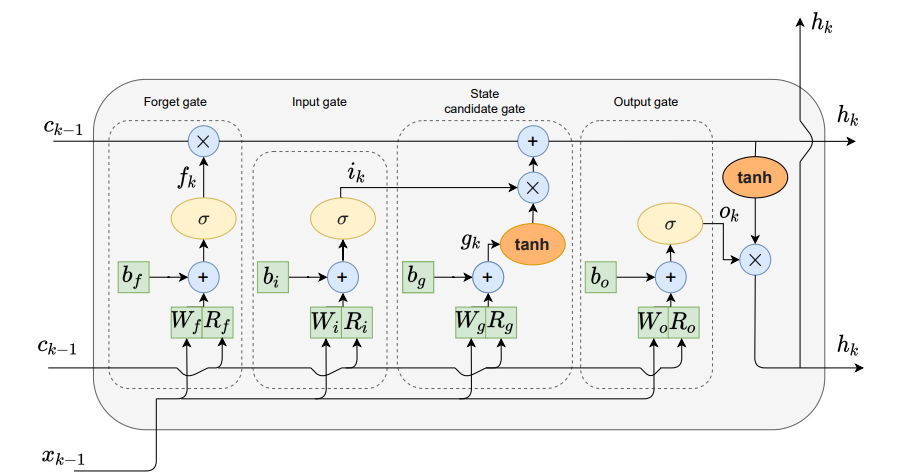
\includegraphics[width=0.75\linewidth]{Images/LSTM_Cell}
    \caption{Internal dataflow of an LSTM cell at time step $t$. The cell state
    $\mathbf{c}_t$ (horizontal channel) carries long-range memory; the forget gate
    $\mathbf{f}_t$, input gate $\mathbf{i}_t$, and output gate $\mathbf{o}_t$
    regulate what is erased, written, and read at each step. The hidden state
    $\mathbf{h}_t$ is derived from the cell state via the output gate.}
    \label{fig:lstm_cell}
    \end{figure}

    \noindent 
    The total parameter count for a single LSTM layer is $4(n_x d + d^2 + d)$, four times that of the basic RNN. This additional capacity improves the modelling of long-range dependencies but increases both memory requirements
    and training time substantially. The Gated Recurrent Unit, introduced in the following section, addresses this cost by merging the cell and hidden states into a single vector and replacing the four-gate mechanism with two gates, reducing the parameter count to $3(n_x d + d^2 + d)$ without significant loss in modelling performance \citep{chung2014empirical}. \\

    \section*{Gated Recurrent Units}

    The \textbf{Gated Recurrent Unit} (GRU) was introduced by \citet{cho2014learning} as a simplified gating architecture that mitigates the vanishing gradient problem whilst retaining fewer parameters than the Long Short-Term Memory network \citep{hochreiter1997long}. The GRU controls information flow through two learned gating vectors, an \textbf{update gate} $\mathbf{z}_t$ and a \textbf{reset gate} $\mathbf{r}_t$, both of which take values in $(0, 1)^d$ and operate element-wise on the hidden state. \\

    \noindent 
    At each time step $t$, given input $\mathbf{x}_t \in \mathbb{R}^{n_x}$ and previous hidden state $\mathbf{h}_{t-1} \in \mathbb{R}^d$, the GRU computes:

    \begin{align}
    \mathbf{z}_t &= \sigma\!\left(W_z\, \mathbf{x}_t
    + U_z\, \mathbf{h}_{t-1} + \mathbf{b}_z\right), \label{eq:gru_update} \\
    \mathbf{r}_t &= \sigma\!\left(W_r\, \mathbf{x}_t
    + U_r\, \mathbf{h}_{t-1} + \mathbf{b}_r\right), \label{eq:gru_reset} \\
    \tilde{\mathbf{h}}_t &= \tanh\!\left(W_h\, \mathbf{x}_t
    + U_h\,(\mathbf{r}_t \odot \mathbf{h}_{t-1}) + \mathbf{b}_h\right),
    \label{eq:gru_candidate} \\
    \mathbf{h}_t &= (1 - \mathbf{z}_t) \odot \mathbf{h}_{t-1}
    + \mathbf{z}_t \odot \tilde{\mathbf{h}}_t, \label{eq:gru_hidden}
    \end{align}

    \noindent 
    where $\sigma$ is the sigmoid function, $\odot$ denotes the Hadamard (element-wise) product, and $W_z, W_r, W_h \in \mathbb{R}^{n_x \times d}$ and $U_z, U_r, U_h \in \mathbb{R}^{d \times d}$ are learned parameter matrices. The
    computation in Equations~\eqref{eq:gru_update}--\eqref{eq:gru_hidden} admits the following interpretation. \\

    \noindent 
    The \textbf{update gate} $\mathbf{z}_t$ governs how much of the previous hidden state is preserved in the new hidden state. When $\mathbf{z}_t \approx \mathbf{0}$, the hidden state is carried forward unchanged from $\mathbf{h}_{t-1}$; when $\mathbf{z}_t \approx \mathbf{1}$, the hidden state is replaced entirely by the candidate $\tilde{\mathbf{h}}_t$. The network learns to open or close this gate adaptively based on the input and the current state. \\

    \noindent 
    The \textbf{reset gate} $\mathbf{r}_t$ controls how much of the previous hidden state is made available when computing the candidate $\tilde{\mathbf{h}}_t$. When $\mathbf{r}_t \approx \mathbf{0}$, the previous hidden state is suppressed and the candidate is computed as if from a fresh initialisation, allowing the network to discard accumulated context that is no longer relevant. When $\mathbf{r}_t \approx \mathbf{1}$, the full previous state is incorporated.\\

    \noindent 
    The \textbf{candidate hidden state} $\tilde{\mathbf{h}}_t$
    (Equation~\eqref{eq:gru_candidate}) is a $\tanh$-activated combination of the
    current input and the gated previous state. It represents the new information that
    could potentially enter the hidden state at this time step. \\

    \noindent 
    The \textbf{final hidden state} $\mathbf{h}_t$ (Equation~\eqref{eq:gru_hidden})
    is a convex interpolation between the previous hidden state and the candidate,
    with interpolation weights determined by the update gate. Crucially, this
    interpolation creates a near-direct path from $\mathbf{h}_{t-1}$ to $\mathbf{h}_t$
    whenever $\mathbf{z}_t$ is small. When unrolled across $T$ steps, this path
    prevents the gradient from vanishing: the derivative
    $\partial \mathbf{h}_t / \partial \mathbf{h}_{t-k}$ is no longer a product of
    $k$ Jacobians but instead accumulates additively, much as residual connections do
    in feedforward networks. This is the mechanism by which the GRU addresses the
    fundamental limitation of the basic RNN.

    The total number of learnable parameters in a single GRU layer with input dimension
    $n_x$ and hidden dimension $d$ is $3(n_x d + d^2 + d)$, corresponding to the three
    sets of weight matrices and bias vectors in Equations~\eqref{eq:gru_update},
    \eqref{eq:gru_reset}, and \eqref{eq:gru_candidate}. This is two-thirds the parameter
    count of an equivalent LSTM layer, which maintains both a hidden state and a separate
    cell state \citep{chung2014empirical}. Empirical comparisons indicate that the GRU
    matches LSTM performance on many sequence modelling tasks whilst being faster to
    train, a finding that motivates its use in the computationally intensive xVA context
    of this study \citep{chung2014empirical}.

    For a multi-layer GRU, the hidden state $\mathbf{h}_t^{(\ell)}$ at layer $\ell$
    takes the hidden state $\mathbf{h}_t^{(\ell-1)}$ from the layer below as its input
    $\mathbf{x}_t$, stacking the recurrent computation across depth. The output of the
    GRU at each time step $t$ is typically a linear function of the final-layer hidden
    state $\mathbf{h}_t^{(L)}$, and for sequence-to-one prediction tasks (such as
    predicting a scalar xVA quantity from a simulated path), the hidden state at the
    terminal time step $\mathbf{h}_T^{(L)}$ is passed to a feedforward output layer.

    \begin{figure}[htbp]
    \centering
    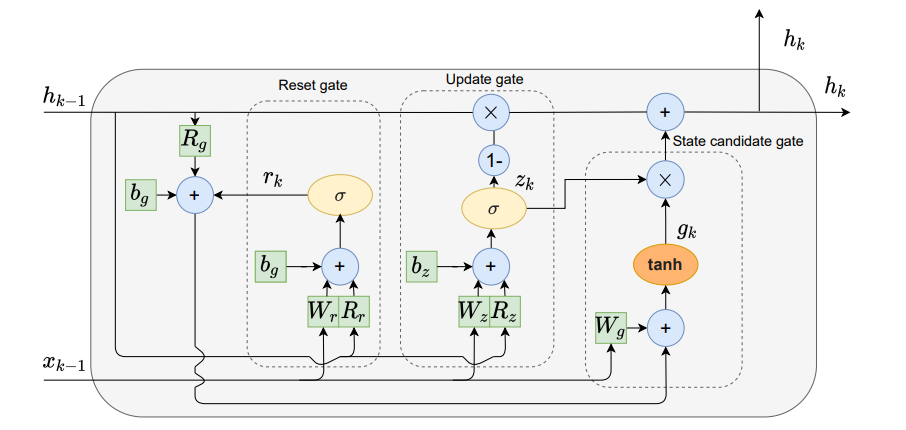
\includegraphics[width=0.75\linewidth]{Images/GRU_Cell}
    \caption{Internal dataflow of a GRU cell at time step $t$. The update gate
    $\mathbf{z}_t$ interpolates between the previous state $\mathbf{h}_{t-1}$
    (weighted by $1 - \mathbf{z}_t$) and the candidate $\tilde{\mathbf{h}}_t$
    (weighted by $\mathbf{z}_t$). The reset gate $\mathbf{r}_t$ controls how
    much of $\mathbf{h}_{t-1}$ enters the candidate computation. The near-direct
    path from $\mathbf{h}_{t-1}$ to $\mathbf{h}_t$ when $\mathbf{z}_t \approx 0$
    is the mechanism that prevents gradient vanishing across long sequences.}
    \label{fig:gru_cell}
    \end{figure}

    \section*{Optimisation}

    \subsection*{Gradient Descent Variants}

    Full-batch gradient descent computes the exact gradient of the loss over all $N$
    training samples before updating weights. This is computationally expensive per
    step and slow to converge when $N$ is large. \textbf{Stochastic gradient descent}
    (SGD) updates weights after every single training sample, approximating the
    gradient with a high-variance single-sample estimate. This is cheap per step but
    introduces substantial noise into the optimisation trajectory.

    \textbf{Mini-batch gradient descent} balances these extremes. Weights are updated
    after processing a mini-batch of $M$ samples, where $1 < M \ll N$. The averaged
    gradient

    \[
    \overline{g}_{w_{mn}} = \frac{1}{M} \sum_{i=1}^{M}
    \frac{\partial L^{(i)}}{\partial w_{mn}}\bigg|_\mathbf{W}
    \]

    is a lower-variance estimate than the single-sample SGD gradient, whilst updates
    remain frequent enough to exploit gradient information efficiently. Mini-batch
    training also maps naturally to GPU parallelism and is the standard approach
    in practice \citep{goodfellow2016deep}.

    \subsection*{Adaptive Learning Rate Methods}

    The Adam optimiser \citep{kingma2015adam} augments mini-batch gradient descent
    with adaptive per-parameter learning rates. Adam maintains exponentially decaying
    averages of past gradients (first moment $m_t$) and past squared gradients (second
    moment $v_t$):

    \begin{align*}
    m_t &= \beta_1 m_{t-1} + (1 - \beta_1)\, g_t, \\
    v_t &= \beta_2 v_{t-1} + (1 - \beta_2)\, g_t^2,
    \end{align*}

    with bias-corrected estimates $\hat{m}_t = m_t/(1 - \beta_1^t)$ and
    $\hat{v}_t = v_t/(1 - \beta_2^t)$. The parameter update is

    \[
    \theta_t = \theta_{t-1} - \frac{\eta}{\sqrt{\hat{v}_t} + \epsilon}\, \hat{m}_t,
    \]

    with standard defaults $\beta_1 = 0.9$, $\beta_2 = 0.999$, $\epsilon = 10^{-8}$
    \citep{kingma2015adam}. The second moment normalises the step size
    per-parameter: directions with consistently large gradients are taken with smaller
    effective learning rates, whilst directions with small or noisy gradients are
    amplified. Adam is robust across a wide range of architectures and is used as
    the default optimiser in this study.

    \section*{Regularisation and Generalisation}

    \subsection*{Overfitting and the Bias-Variance Tradeoff}

    A network trained to minimise training loss can memorise the training data,
    including noise, and perform poorly on previously unseen inputs. This is
    \textbf{overfitting}. The underlying tension is between bias and variance
    \citep{hastie2009elements}: a low-capacity model is biased toward simpler
    functions and may underfit (high training error regardless of data volume);
    a high-capacity model can represent complex functions but absorbs noise in
    the training data, producing high variance in predictions on new inputs.

    The standard diagnostic is to monitor training loss $L_T$ and validation loss
    $L_V$ across epochs. Both decrease initially as the network learns the underlying
    function. When $L_V$ begins to increase whilst $L_T$ continues to fall, the
    network is fitting noise. Training is stopped at the epoch of minimum $L_V$:
    this is \textbf{early stopping}, which uses the validation set as a proxy for
    generalisation performance.

    \subsection*{Weight Regularisation}

    Explicit regularisation modifies the loss function to penalise large weights,
    reducing the effective capacity of the network. The two standard forms are:

    \[
    L_2(\mathbf{y}, \mathbf{t}) = L(\mathbf{y}, \mathbf{t}) + \frac{\lambda}{2}
    \sum_{\text{all } w_{mn}} w_{mn}^2,
    \]

    \[
    L_1(\mathbf{y}, \mathbf{t}) = L(\mathbf{y}, \mathbf{t}) + \lambda
    \sum_{\text{all } w_{mn}} |w_{mn}|.
    \]

    Under $L_2$ regularisation, the modified weight update includes a shrinkage
    term proportional to the current weight:
    $w_{mn} \leftarrow w_{mn} - \eta(\partial L/\partial w_{mn}) - \eta\lambda w_{mn}$.
    This is called \textbf{weight decay}, and its effect is to pull all weights toward
    zero proportionally to their magnitude, preventing any single weight from
    becoming excessively large. Under $L_1$ regularisation, the update instead
    subtracts a constant-sign term:
    $w_{mn} \leftarrow w_{mn} - \eta(\partial L/\partial w_{mn}) - \eta\lambda
    \operatorname{sign}(w_{mn})$. The $L_1$ penalty drives small weights to exactly
    zero, producing sparse weight configurations. The regularisation coefficient
    $\lambda$ is a hyperparameter tuned using the validation set
    \citep{hastie2009elements}.

    \subsection*{Dataset Partitioning}

    Training a network that generalises requires discipline in how data is used.
    The dataset is partitioned into three disjoint subsets: the \textbf{training set},
    used to update weights; the \textbf{validation set}, used to monitor overfitting
    and tune hyperparameters; and the \textbf{test set}, used once at the conclusion
    of training to report final model performance. A typical partition is 50\% training,
    25\% validation, and 25\% test, with all subsets drawn randomly from the full
    dataset. Using the test set during model development invalidates its role as an
    unbiased estimator of generalisation error.

    When training data is limited, $k$-fold cross-validation provides more reliable
    generalisation estimates. The dataset is divided into $k$ equal folds and the
    training-testing procedure is repeated $k$ times, each time holding out a different
    fold. The performance metric is averaged over all $k$ rounds, and every data point
    is used for testing exactly once \citep{hastie2009elements}.

    \section*{Data Preparation}

    Neural network training is sensitive to the scale of input features. When features
    span very different numerical ranges, the contributions of different inputs to the
    pre-activation at the first hidden layer are unequal. Inputs with large magnitudes
    dominate the activation and drive the weight updates during early training, whilst
    the network is slow to resolve the influence of smaller-valued inputs. Normalising
    all features to a common scale before training reduces this problem and improves
    convergence.

    Two methods are standard. \textbf{Min-max normalisation} maps each feature to
    the interval $[0, 1]$:

    \[
    \tilde{d} = \frac{d - d_{\min}}{d_{\max} - d_{\min}}.
    \]

    \textbf{Z-score standardisation} rescales each feature to zero mean and unit
    variance:

    \[
    \tilde{d} = \frac{d - \mu}{\sigma},
    \]

    where $\mu$ and $\sigma$ are the sample mean and standard deviation computed from
    the training set. Both transformations are invertible, so predictions in the
    normalised space can be mapped back to original units. Z-score standardisation
    is generally preferred when the input distribution is not bounded and may be
    approximately Gaussian \citep{goodfellow2016deep}. In the context of this study,
    input features include short rates, time-to-maturity, and notionals, which span
    several orders of magnitude and are standardised prior to network training. Target
    prices are likewise normalised to improve numerical conditioning of the
    optimisation.

    \section*{Summary}

    This chapter has developed the theoretical machinery of neural networks and deep
    learning that underpins the surrogate pricing methodology of this study. Beginning
    with the artificial neuron and the perceptron learning rule, we have established how
    multi-layer architectures achieve non-linear function approximation. The Universal
    Approximation Theorem provides the existence guarantee that justifies applying
    neural networks to continuous pricing functions defined on compact domains.
    Backpropagation operationalises gradient descent by efficiently computing parameter
    gradients via the chain rule, with explicit delta formulas derived for MSE and
    cross-entropy losses.

    The feedforward MLP, whilst theoretically expressive, treats observations as
    independent. For pricing problems indexed by a simulation time grid, a recurrent
    architecture is more natural. The Gated Recurrent Unit addresses the vanishing
    gradient limitation of the basic RNN through an update gate and a reset gate, which
    create direct gradient pathways across time steps and allow the network to
    selectively retain or discard accumulated context. Mini-batch optimisation with
    Adam, combined with $L_2$ regularisation and early stopping, addresses the
    practical challenges of training on finite datasets. Data normalisation ensures
    numerical stability when inputs span disparate scales.

    With these foundations established, the following chapter presents the differential
    deep learning framework of \citet{mrad2025differential}, which augments the
    surrogate architecture with pathwise sensitivity information, enabling simultaneous
    approximation of prices and Greeks from a single trained network with substantially
    improved sample efficiency.


        

\part{Literature Review}
%    \section{Notes}

\section{Implementation 1a—Approximating semi-analytical solution}\label{sec:model1a}
    In this section, we will detail the implementation of training a surrogate model to learn the exposure profiles of an interest rate swap. We then detail the implementation of deep learning methods that can be used to learn these exposure profiles and motivate their application. \\

    \noindent
    First, we note that computing the exposure of a derivative product is not always available in closed form. As \cite{Gregory_2015} explains, at its core, the problem of computing exposures is fundamentally an option pricing problem,  
    \begin{equation}
        \text{Exposure} = \text{max(value,0)}
    \end{equation}
    The expression above captures the loss we would incur if the contract had positive value at the time of default. This payoff structure can be likened to holding a short option position. Conversely, when the contract value is negative, we are effectively long an option on our own default. However, it cannot be treated as such because of the complexity of the underlying products and the components that drive xVA calculations. This can be illustrated by considering a vanilla interest rate swap, which can be represented linearly as a portfolio of consecutive forward rate agreements (FRAs), as shown in \ref{eq:swp_linear_fras}. The exposure at time $t$ is defined as the positive part of the swap value,
    \begin{equation}
        \text{Exposure} = \max(V^{Swp}(t),0)
    \end{equation}
    Although the price of an interest rate swap is linear and admits a closed-form expression, the exposure defined above introduces a non-linearity due to the presence of the maximum operator.
    Drawing upon the frameworks of \cite{sorensen1994pricing} and \cite{jamshidian1989exact}, we derive a semi-analytical solution for computing the exposure profile of an interest rate swap.  \\
    
    \begin{lemma}\label{lem:swapEE_equivalent_swaption}
    
    Let $V^{Swp}(t)$ be the value at time $t$ of an interest rate swap under the risk–neutral measure $\mathbb{Q}$\\
    \[
    EE(t_0,t) = \mathbb{E}^{\mathbb{Q}}\!\left[\max\!\left(V^{Swp}(t),0\right)\,\Big|\,\mathcal{F}_{t_0}\right]
    \]
     \noindent
     Let $M(t)$ denote the money–market account and $P(t,T)$ the zero–coupon bond price. Then, the expected exposure at time $t$ for an interest rate swap can be expressed in terms of European-style swaptions as follows,

    \begin{align*}
        EE(t_0,t)  &= \mathbb{E}^{\mathbb{Q}} \Bigg[ \frac{M(t_0)}{M(t)} \max \Big( V^{SWP}(t),0 \Big) \Big| \mathcal{F}_{t_0} \Bigg],\\
        &= \mathbb{E}^{\mathbb{Q}} \Bigg[ \frac{M(t_0)}{M(t)} \max \Big(N \cdot \sum_{k=i+1}^{m} \tau_{k} P(t,T_k) (\ell(t,T_{k-1},T_k) - K),0 \Big) \Big| \mathcal{F}_{t_0} \Bigg],\\
        &= \mathbb{E}^{\mathbb{Q}} \Big[ \frac{1}{M(t)} V^{Swpt}(t,K) \Big | \mathcal{F}_{t_0}\Big]
    \end{align*}
   where $V^{\text{Swpt}}(t, K)$ represents the time $t$ value of a European swaption with strike rate $K$ and exercise date $t$.
    
    \end{lemma}

    \noindent
    Following the techniques of \cite{jamshidian1989exact}, we derive the price of the swaption under the Hull-White model. To do this, we will have to find the value of the swaption presented in lemma\ref{lem:swapEE_equivalent_swaption} in terms of zero-coupon bond prices under the $T_i$-forward measure $\mathbb{Q}^{T_i}$.

    \begin{equation}
    V^{\text{Swpt}}(t_0) = N \cdot P(t_0, T_i) \times \mathbb{E}^{T_i} \left[ \max \left( \sum_{k=i+1}^m \tau_k P(T_i, T_k) \left( \ell(T_i; T_{k-1}, T_k) - K \right), 0 \right) \middle| \mathcal{F}(t_0) \right]
    \end{equation}

    \noindent
    The term inside the maximum function represents the present value of the swap's future cash flows at time $T_i$, this summation simplifies to an expression involving only zero-coupon bond prices, yielding,
    \begin{align}
    \sum_{k=i+1}^m \tau_k P(T_i, T_k) \left( \ell_k(T_i) - K \right) &= 1 - P(T_i, T_m) - K \sum_{k=i+1}^m \tau_k P(T_i, T_k),\\
    &= 1 - \sum_{k=i+1}^m c_k P(T_i, T_k)
    \end{align}

    \noindent
    Where $c_k$ are the coupons \( c_k = K \tau_k \) for \( k = i+1, \ldots, m-1 \) and \( c_m = 1 + K \tau_m \). The value of the swaption in terms of ZCB $P(T_i,T_k)$ can thus be expressed as 
    
    \begin{equation}
        V^{\text{Swpt}}(t_0) = N \cdot P(t_0, T_i) \mathbb{E}^{T_i} \left[ \max \left( 1 - \sum_{k=i+1}^m c_k P(T_i, T_k), 0 \right) \middle| \mathcal{F}(t_0) \right]
    \end{equation}

    \noindent
    As the ZCB \( P(T_i, T_k) \) in the case of an affine short-rate process \( r(t) \) can be expressed as
    \begin{equation}
        P(T_i, T_k) = \exp\left(\bar{A}_r(\bar{\tau}_k) + \bar{B}_r(\bar{\tau}_k)r(T_i)\right),
    \end{equation}

    \noindent
    with \( \bar{\tau}_k := T_k - T_i \), the (scaled) pricing equation is written as 
    \begin{equation}
        V^{\text{Swpt}}(t_0) = P(t_0, T_i) \cdot N \cdot \mathbb{E}^{T_i} \left[ \max\left(1 - \sum_{k=i+1}^m c_k e^{\bar{A}_r(\bar{\tau}_k) + \bar{B}_r(\bar{\tau}_k)r(T_i)}, 0\right) \middle| \mathcal{F}(t_0) \right]
    \end{equation}

    \noindent
    An expression of this form was solved in \cite{jamshidian1989exact}, who showed that under an affine one-factor model, the option on a portfolio of zero-coupon bonds can be decomposed into a portfolio of options on the individual bonds. This decomposition proceeds by first finding the critical short rate \( r^*(T_i) \) that satisfies \( \sum_{k=i+1}^m c_k P(T_i, T_k; r^*(T_i)) = 1 \), after which the swaption value reduces to a sum of bond options exercised when the corresponding bond price falls below a strike. Following \cite{oosterlee2019mathematical}, since each function \( f_k(r) \) is strictly increasing in the interest rate \( r \), their sum \( \sum_{k} f_k(r) \) is also strictly increasing. This monotonicity guarantees the existence of a unique critical interest rate \( r^* \) that satisfies
    
    \begin{equation}
        \sum_{k} f_k(r^*) = K
    \end{equation}   

    \noindent
    where \( K \) represents the strike level. The value of \( r^* \) can be found numerically using standard root-finding techniques, such as the Newton-Raphson method.

    \noindent
    Using this critical rate, the payoff function can be reformulated so that the maximum term becomes
    \begin{gather}
        \max\left( \sum_{k} f_k(r^*) - \sum_{k} f_k(r), 0 \right) = \max\left( \sum_{k} \left( f_k(r^*) - f_k(r) \right), 0 \right)
    \end{gather}

    \noindent
     because, the sum is increasing monotonically, the condition \( \sum_{k} f_k(r^*) > \sum_{k} f_k(r) \) holds precisely when \( r < r^* \). Consequently, the payoff simplifies to
   \begin{equation}
       \sum_{k} \left( f_k(r^*) - f_k(r) \right) \cdot \mathbb{1}_{\{ r < r^* \}}
   \end{equation} 
   
    \noindent
    where \( \mathbb{1}_{\{ r < r^* \}} \) is an indicator function that takes the value one when the interest rate is below the critical threshold and zero otherwise. \\
    \begin{equation}
        V^{\text{Swpt}}(t_0) = P(t_0, T_i) \cdot N \cdot \sum_{k=i+1}^m c_k \mathbb{E}^{T_i} \left[ \max \left( \hat{K}_k - e^{\bar{A}_r(\bar{\tau}_k) + \bar{B}_r(\bar{\tau}_k) r(T_i)}, 0 \right) \right]
    \end{equation}

    \noindent
    with \(\hat{K}_k := \exp \left( \bar{A}_r(\bar{\tau}_k) + \bar{B}_r(\bar{\tau}_k) r^* \right)\), where the parameter \(r^*\) is chosen such that
    \begin{equation}
        \sum_{k=i+1}^m c_k \exp \left( \bar{A}_r(\bar{\tau}_k) + \bar{B}_r(\bar{\tau}_k) r^* \right) = 1
    \end{equation}
    
    \noindent
    To finally obtain the pricing formula for the swaption, note that each term in the summation now takes the form of an expectation involving a single zero-coupon bond price. Each element of this sum represents a European put option on a zero-coupon bond, with strike price \(\hat{K}_k\) and maturity \(T_i\). That is,
    \begin{equation}
        V_p^{\text{ZCB}}(t_0, T_i) = P(t_0, T_i) \cdot \mathbb{E}^{T_i} \left[ \max \left( \hat{K}_k - e^{\bar{A}_r(\bar{\tau}_k) + \bar{B}_r(\bar{\tau}_k) r(T_i)}, 0 \right) \right]
    \end{equation}

    \noindent
    with \(\bar{\tau}_k = T_k - T_i\). The quantity inside the expectation now includes the \(\hat{K}_k\) against the discounted bond price at time \(T_i\), which is expressed in terms of the short rate \(r(T_i)\).\\

    \noindent
    Using the results from \cite{jamshidian1989exact}, we have now transformed a single complex option on a portfolio of bonds into a portfolio of simpler options on individual bonds. Under the Hull-White model, pricing European options on zero-coupon bonds admits a closed-form solution. This is because the affine structure of the model ensures that zero-coupon bond prices are log-normally distributed under the forward measure.\\   

    \noindent
    A European swaption thus simplifies to a weighted sum of these individual bond option prices
    \begin{equation}
        V^{\text{Swpt}}(t_0) = N \cdot \sum_{k=i+1}^m c_k V_p^{\text{ZCB}}(t_0, T_k)
    \end{equation}
    
    \noindent
     In the literature, two related exposure measures appear, the undiscounted expected exposure, $EE(t_0,t) = \mathbb{E}^{\mathbb{Q}}[\max(V(t),0)|\mathcal{F}_{t_0}]$, represents the expected replacement cost at future time $t$. For xVAs calculations, however, the discounted expected exposure, $DEE(t_0,t) = \mathbb{E}^{\mathbb{Q}}[D(0,t)\max(V(t),0)|\mathcal{F}_{t_0}]$, is required as it represents the present value of future exposure.\\

    \noindent
    A key observation from Lemma~\ref{lem:swapEE_equivalent_swaption} is that $DEE(T_i)$ equals the price of a European payer swaption with expiry $T_i$. This equivalence provides a convenient analytical benchmark for our surrogate modeling approach. The undiscounted exposure is then recovered by dividing by the discount factor: $EE(T_i) = DEE(T_i)/P(0,T_i)$.\\
    
    \noindent
    Step 1: Coupon bond representation. A payer swaption with expiry $T_e$ on a swap with payments $\{c_k\}$ at dates $\{T_k\}$ has payoff:
    
    \begin{equation}
        \max\!\left(1 - \sum_k c_k \, P(T_e, T_k),\; 0\right)
    \end{equation}

    \noindent
    where $c_k = \delta K$ for $k < n$ and $c_n = \delta K + 1$ final coupon plus principal. The exercise condition is equivalent to the coupon bond $\sum_k c_k \, P(T_e, T_k) < 1$. \\

    \noindent
    Step 2: Critical rate $r^*$. Because each $P(T_e, T_k) = A(T_e,T_k) \exp\!\bigl(-B(T_e,T_k) r\bigr)$ is strictly decreasing in $r$, the coupon bond value is also strictly decreasing in $r$. There exists a unique $r^*$ such that:

    \begin{equation}
        \sum_k c_k \, A(T_e,T_k) \exp\!\bigl(-B(T_e,T_k) r^*\bigr) = 1
    \end{equation}
    This is solved numerically. The exercise region is $\{r(T_e) > r^*\}$ for a payer swaption.

    \noindent
    Step 3: Decomposition into ZCB options. Define strike prices $X_k = A(T_e,T_k) \exp\!\bigl(-B(T_e,T_k) r^*\bigr)$. Then:
    \begin{equation}
        \text{Swaption}_{\text{payer}} = \sum_k c_k \; \text{Put}(0; T_e, T_k, X_k)
    \end{equation}

    \noindent
    where $\text{Put}(0; T_e, T_k, X_k)$ is the price of a European put option on the zero-coupon bond $P(T_e, T_k)$ with strike $X_k$ and expiry $T_e$. This decomposition is exact because at $r = r^*$, each bond is at its individual strike, and the monotonicity ensures all bonds are simultaneously above/below their strikes.\\

    \noindent
    Step 4: ZCB option pricing. Each put option has the closed-form solution \citep{hull1994numerical}:
    \begin{equation}
        \text{Put}(0; T_e, T, X) = X \, P_{mkt}(0,T_e) \, \Phi(-d_2) - P_{mkt}(0,T) \, \Phi(-d_1)
    \end{equation}
    where
    \begin{equation}
            d_1 = \frac{\ln\!\left(\displaystyle\frac{P^M(0,T)}{X\,P^M(0,T_e)}\right)}{\sigma_P} + \frac{\sigma_P}{2}, \qquad
    d_2 = d_1 - \sigma_P,
    \end{equation}
    \begin{equation}
        \sigma_P = \sigma \; B(T_e,T) \; \sqrt{\frac{1 - e^{-2a T_e}}{2a}}
    \end{equation}
    Here $\sigma_P$ is the volatility of the log zero‑coupon bond price at the option expiry, and $\Phi$ is the standard normal CDF.\\

    \noindent
    \textbf{Implementation:} \texttt{SwaptionPricer.price()} implements all four steps in a vectorised manner. The critical rate $r^*$ is found via Newton's method with analytical Jacobian (quadratic convergence), falling back to Brent's method.
    
    \subsection*{Complete Pipeline}
    
    The full computation for one (date, $a$, $\sigma$) sample proceeds as:
    \begin{enumerate}
        \item \textbf{Input:} Market ZCB curve $P^M(0,T_k)$ for 40 quarterly tenors, HW parameters $(a,\sigma)$.
        \item \textbf{Curve fitting:} Fit a cubic spline to $\ln P^M$, extract $f(0,t)$ and $r(0)$ $\rightarrow$ \texttt{HullWhiteAnalytical}.
        \item \textbf{Par rate:} Compute $K^* = \bigl(P^M(0,0) - P^M(0,10)\bigr) / A(0)$ $\rightarrow$ \texttt{SwapPricer.par\_rate()}.
        \item \textbf{For each monitoring date $T_i \in \{0.25, 0.50, \dots, 10.00\}$:}
            \begin{itemize}
                \item Price payer swaption$(0; T_i, 10, K^*)$ via Jamshidian $\rightarrow$ $\text{DEE}(T_i)$.
                \item $\text{UEE}(T_i) = \text{DEE}(T_i) / P^M(0,T_i)$.
            \end{itemize}
        \item \textbf{Output:} 40‑dimensional UEE vector.
    \end{enumerate}
    This produces 40 UEE values per sample, yielding the target labels for the surrogate model.

    

\newpage
\section{Implementation 1b—Approximating Exposure Profiles from Hull-White model}\label{sec:model1b}
    While the analytical approach (Section~\ref{sec:model1a}) is computationally efficient, it is limited to European-style exercise and specific model assumptions. Monte Carlo simulation provides a general-purpose alternative that accommodates arbitrary payoff structures and path-dependent features. This section details the Monte Carlo framework for computing exposure profiles under the Hull-White one-factor model.\\
      \noindent
  In the above, we are averaging future mark-to-market values over all continuous paths of price factors. Mathematically, for each market scenario and at each time step, we compute the value of the financial derivative. We approximate the conditional expectation via Monte Carlo simulation, but this creates a nested structure: for every outer scenario at every future date, we require an inner simulation to estimate the conditional expectation. The computational cost of this nested framework is governed by the following quantities:
 
\begin{itemize}
      \item $N$: the number of outer simulation paths (market scenarios from $t_0$ to $t_M$),
      \item $M$: the number of future simulation dates $\{t_1, t_2, \dots, t_M\}$ with $t_M = T$,
      \item $K$: the number of inner paths used at each valuation point $(i, k)$ to estimate the conditional expectation,
      \item $d$: the dimension of the state vector $X(t)$.
  \end{itemize}

  \newpage
  \caption{Estimation of $V(t_k, \{X(t_j)\}_{j=1}^{k})$}                                                               \noindent
  Algorithm~\ref{alg:valuation} presents the inner Monte Carlo procedure for estimating the value at a single point $(i, k)$.

  \begin{algorithm}
  \caption{Estimation of $V(t_k, \{X(t_j)\}_{j=1}^{k})$ at a fixed outer scenario $i$ and time step $t_k$}
  \label{alg:valuation}
  \begin{algorithmic}[1]
      \Require Observed path $\{x_j\}_{j=1}^{k}$ up to time $t_k$, risk-neutral dynamics $\mathbb{Q}$, number of inner paths $K$, time grid $\{t_k, t_{k+1}, \ldots, t_M\}$ with $t_M = T$,
  payoff function $g$ defined by the instrument's contractual terms
      \Ensure $\hat{V}$ -- a Monte Carlo estimate of $\mathbb{E}^{\mathbb{Q}}\!\Big[ V^{MTM}\!\big(t_k, \{X(t)\}_{t \leq t_k}\big) \;\Big|\; \{X(t_j) = x_j\}_{j=1}^{k} \Big]$
      \State Initialise accumulator $S \leftarrow 0$
      \For{$i = 1, 2, \ldots, K$}
          \State Set $X^{(i)}(t_k) \leftarrow x_k$
          \For{$m = k, k+1, \ldots, M-1$}
              \State Simulate $X^{(i)}(t_{m+1})$ from $X^{(i)}(t_m)$ under $\mathbb{Q}$
          \EndFor
          \State Compute $\text{CF}^{(i)} \leftarrow g\!\Big(\{x_j\}_{j=1}^{k},\; \{X^{(i)}(t_m)\}_{m=k+1}^{M}\Big)$
          \State $S \leftarrow S + \text{CF}^{(i)}$
      \EndFor
      \State $\hat{V} \leftarrow S \,/\, K$
      \State \Return $\hat{V}$
  \end{algorithmic}
  \end{algorithm}
  \noindent
  For a fixed outer scenario $i$ and a fixed time step $t_k$, the algorithm simulates $K$ inner paths, each advancing the $d$-dimensional state vector from $t_k$ to $t_M$ in $M - k$ steps.
  The work at a single valuation point is therefore:

  \begin{equation}
  \text{Work}(i, k) = K \cdot (M - k) \cdot d.
  \end{equation}

  \noindent
  To construct the full valuation grid -- the value at every simulation date on every outer scenario -- we sum over all $N$ outer paths and all $M$ time steps:

  \begin{equation}
  \text{Total work} = \sum_{i=1}^{N} \sum_{k=1}^{M} K \cdot (M - k) \cdot d = N \cdot K \cdot d \sum_{k=1}^{M} (M - k).
  \end{equation}

  \noindent
  Evaluating the sum over $k$:

  \begin{equation}
  \sum_{k=1}^{M} (M - k) = \sum_{j=0}^{M-1} j = \frac{M(M-1)}{2}.
  \end{equation}

  \noindent
  Thus the total computational work is:

  \begin{equation}
  \text{Total work} = N \cdot K \cdot d \cdot \frac{M(M-1)}{2}.
  \end{equation}

  \noindent
  For large $M$, this grows as:

  \begin{equation}
  \text{Total work} = \mathcal{O}\!\left(N \, K \, M^{2} \, d\right).
  \end{equation}

  \noindent
     The cost scales quadratically with the number of simulation dates $M$, since at early time steps (when $k$ is small) each inner path must travel almost the entire remaining time grid to reach maturity. In contrast, the cost scales only linearly with the number of outer scenarios $N$, the number of inner paths $K$, and the dimension of the state vector $d$. This quadratic dependence on $M$ is precisely what we mean by the nested simulation curse: the inner loop must be executed $N \times M$ times, and each execution itself costs $\mathcal{O}(M \cdot d)$ per path, which together give us the $M^2$ factor. It is this cost structure that makes brute-force nested Monte Carlo impractical for routine risk management, and it is what drives the search for approximation methods that can bypass the inner simulation altogether.\\


    \noindent
    We first present the solution of the Hull-White model. To solve this linear SDE \ref{eq:hull_white}, we employ an integrating factor. Define the process

    \begin{equation}
        y(t) = e^{a t} r(t). 
    \end{equation}

    \noindent
    Applying Itô's lemma to \(y(t)\) gives

    \begin{equation}
        dy(t) = a e^{a t} r(t) dt + e^{a t} dr(t) = a y(t) dt + e^{a t} dr(t).
    \end{equation}

    \noindent
    Substituting the SDE for \(dr(t)\):
    \begin{equation}
        dy(t) = a y(t)dt + e^{a t}[a (\theta(t) - r(t))dt + \eta dW_r(t)],
    \end{equation}
    We thus obtain the system of equations
    
    \[
    \begin{cases}
    y(t) = e^{a t}r(t), \\
    dy(t) = a\theta(t)e^{a t}dt + \eta e^{a t}dW_r(t).
    \end{cases}
    \]
    The right-hand side of the \( y(t) \)-dynamics does not depend on state vector \( y(t) \), and we can therefore determine the solution of \( y(t) \) by integrating both sides of the SDE,
    
    \begin{equation}
        \int_0^t dy(z) = a \int_0^t \theta(z)e^{a z}dz + \eta \int_0^t e^{a z}dW_r(z),
    \end{equation}

    \noindent
    which gives us,
    
    \begin{equation}
        y(t) = y(0) + a \int_0^t \theta(z)e^{a z}dz + \eta \int_0^t e^{a z}dW_r(z)
    \end{equation}

    \noindent
    By the definition of \( y(t) \), with \( y(0) = r_0 \), the solution for the process \( r(t) \) is given by 

    \begin{equation}
        r(t) = e^{-a t}r_0 + a \int_0^t \theta(z)e^{-a(t-z)}dz + \eta \int_0^t e^{-a(t-z)}dW_r(z)
    \end{equation}

    \begin{equation}
        \mathbb{E}[r(t)|\mathcal{F}(t_0)] = r_0 e^{-a t} + a \int_0^t \theta(z) e^{-a(t-z)} dz
    \end{equation}

    \noindent 
    For simulation purposes, we need to generate paths of the short rate \(r(t)\) at discrete dates. Under the Hull‑White model (Equation~\ref{eq:hull_white}), the short rate is a Gaussian process, and its transition density is known in closed form.  This allows us to simulate exactly without time‑stepping bias. \\

    
    \noindent
    Let the simulation dates be \(t_0 < t_1 < \dots < t_M\) with constant step \(\Delta = t_{k+1} - t_k\).  Conditional on the value at time \(t_k\), the short rate at \(t_{k+1}\) is normally distributed:

    \begin{equation}
        r(t_{k+1}) \mid r(t_k) \;\sim\; \mathcal{N}\!\left( r(t_k)e^{-a\Delta} + \Theta(t_k,\Delta),\; \Sigma^2(\Delta) \right)
    \end{equation}
        
    where
    \begin{equation}
            \Theta(t_k,\Delta) = \int_{t_k}^{t_{k+1}} e^{-a(t_{k+1}-u)}\theta(u)\,du, \qquad \Sigma^2(\Delta) = \frac{\sigma^2}{2a}\bigl(1-e^{-2a\Delta}\bigr)
    \end{equation}
    \noindent
    The drift term \(\Theta(t_k,\Delta)\) can be expressed in terms of the initial instantaneous forward curve \(f(0,t)\) (which is calibrated from market data).  Using the relation between \(\theta(\cdot)\) and the forward curve, one obtains the explicit formula

    \begin{equation}
            \Theta(t_k,\Delta) = f(0,t_{k+1}) - f(0,t_k)e^{-a\Delta} + \frac{\sigma^2}{2a^2}\bigl(1-e^{-a\Delta}\bigr)\bigl(1-e^{-a(2t_k+\Delta)}\bigr)
    \end{equation}
    
    \noindent
    The conditional variance is independent of the current time and is given by
    \begin{equation}
        \Sigma(\Delta) = \sigma\sqrt{\frac{1-e^{-2a\Delta}}{2a}}
    \end{equation}

    \noindent
    Therefore, for each path and each time step we generate an independent standard normal draw \(Z_{k} \sim \mathcal{N}(0,1)\) and update the short rate via
    \begin{equation}
         r(t_{k+1}) = r(t_k)e^{-a\Delta} + \Theta(t_k,\Delta) + \Sigma(\Delta)\,Z_{k}
    \end{equation}
    
    \noindent
    This exact discretization, which is efficient and unbiased.  In practice, the forward curve \(f(0,t)\) is interpolated from observed market rates (e.g., OIS or LIBOR curves) and the parameters \(a\) and \(\sigma\) are calibrated to swaption prices.  The simulation then proceeds forward in time, producing the outer scenarios required for exposure computation.\\

    \noindent
    Once we have generated the outer scenarios and valued the interest rate swap on each path at every monitoring date, we proceed to compute the exposure metrics. For a given path \(m\) and time step \(t_k\), the \textbf{positive exposure} is defined as:
    \begin{equation}
        E^m(t_k) = \max(V^m(t_k), 0)
        \label{eq:positive_exposure}
    \end{equation}
    where \(V^m(t_k)\) denotes the swap value on path \(m\) at time \(t_k\). \\
    
    \noindent
    Averaging these positive exposures across all Monte Carlo paths yields the Undiscounted Expected Exposure (UEE) at time \(t_k\):
    \begin{equation}
        \text{UEE}(t_k) = \mathbb{E}^\mathbb{Q}[\max(V(t_k), 0)]
        \label{eq:uee}
    \end{equation}
    which is estimated by the Monte Carlo average
    \begin{equation}
        \widehat{\text{UEE}}(t_k) = \frac{1}{M} \sum_{m=1}^{M} E^m(t_k)
        \label{eq:uee_estimate}
    \end{equation}

    \noindent
    where \(M\) is the total number of simulated paths.\\

    \noindent
    If we incorporate discounting, we obtain the Discounted Expected Exposure (DEE)
    \begin{equation}
        \text{DEE}(t_k) = \mathbb{E}^\mathbb{Q}[D(0, t_k) \cdot \max(V(t_k), 0)]
        \label{eq:dee}
    \end{equation}
    estimated by:
    \begin{equation}
        \widehat{\text{DEE}}(t_k) = \frac{1}{M} \sum_{m=1}^{M} D^m(0, t_k) \cdot E^m(t_k)
        \label{eq:dee_estimate}
    \end{equation}
    where \(D^m(0, t_k)\) is the discount factor along path \(m\) from time \(0\) to \(t_k\). \\

    \noindent
    Finally, a key risk metric is the Expected Positive Exposure (EPE), which represents the time-averaged expected exposure over a given period. Following \cite{Gregory_2015}, the EPE is defined as:
    \begin{equation}
        \text{EPE} = \frac{1}{T_{\text{max}} - T_{\text{min}}} \int_{T_{\text{min}}}^{T_{\text{max}}} \text{UEE}(t) \, dt
        \label{eq:epe}
    \end{equation}
    In practice, this integral is approximated using the trapezoidal rule over the discrete monitoring dates.
    
    \newpage 
    
\section{Implementation 2 - Exposure for Bermudan Swaption via Longstaff–Schwartz Monte Carlo}
    \noindent
    The Monte Carlo simulation approach detailed in Section~\ref{sec:model1b} provides a more general-purpose framework capable of handling arbitrary payoff structures and path-dependent features. This section details the Monte Carlo framework for computing exposure profiles for a Bermudan swaption under the Hull-White one-factor model, a problem with a significantly more complex structure than the vanilla swap considered previously. \\

    \noindent
    The Bermudan swaption introduces two layers of complexity. First, the pricing problem itself is non-linear due to the optimal stopping feature, the holder can choose when to exercise, making the contract's value dependent on the entire future evolution of interest rates. This early exercise optionality destroys the linearity that underpins closed-form solutions and necessitates advanced numerical methods such as dynamic programming or regression-based Monte Carlo. Second, when we move from pricing to exposure computation, this non-linearity is compounded by the nested expectation structure inherent in credit risk metrics. \\

    \noindent
    For each future simulation date and for each market scenario, we must determine not only the swap value but also the optimal exercise policy conditional on that specific state, a task that typically requires solving a separate optimal stopping problem at every node. Thus, computing expected exposure for a Bermudan swaption demands a nested simulation within which an optimal stopping problem must be solved at the inner level. This double layer of complexity renders brute-force approaches computationally prohibitive and motivates the need for efficient surrogate methods. In the following, we describe the implementation of a Longstaff–Schwartz Monte Carlo framework adapted for exposure calculations, highlighting the algorithmic choices and computational challenges that arise. \\


\section{Introduction and Problem Formulation}
     Calculating exposure profiles is central to xVA calculations. As outlined in \cite{zhu2007guide}, a generic approach to modelling counterparty credit risk can be detailed as follows:
    
    \begin{itemize}
        \item Scenario generation: this involves simulating the underlying market risk factors on a predetermined set of future dates.
        \item Instrument valuation: on each of the predetermined future dates, and for each realised observation of the underlying market risk factors, we calculate the value of the instrument.
        \item Portfolio aggregation: for each simulation date and each realisation of the underlying market risk factors, the counterparty-level exposure is calculated.
    \end{itemize}

    \noindent
    The price of a financial derivatives contract depends on the realisation of a set of risk factors, such as foreign exchange (FX) rates, interest rates, credit spreads, etc. Given a fixed set of future simulation dates $\{t_k\}_{k=1}^{N}$, we are interested in generating potential market scenarios for each underlying risk factor at these dates. Specifically we model the short-interest rates dynamics under measure $\mathbb{Q}$. A popular choice of modelling short-interest rates is the Hull-White one-factor model given by 
 
    \begin{equation}\label{eq:hull_white}
        dr(t) = \alpha(\theta(t) -  r(t))dt + \sigma dW^\mathbb{Q}(t)
    \end{equation}
    \noindent 
    A layer of complexity is added when considering regulatory standards, which require a more sophisticated approach, a two-factor Hull-White model (G2++) calibrated on real market data \cite{silotto2021everything}. The dynamics of the instantaneous-short-rate process under the risk neutral measure $\mathbb{Q}$ is given by \\
    \begin{equation}
        r(t) = x(t) + y(t) + \varphi (t), \quad r(0) = r_0
    \end{equation}
    \noindent
    where the process $\{ x(t) : t \ge 0\}$ $\{ y(t) : t \ge 0\}$ satisfy 
    \begin{align}
        dx(t) &= -ax(t)dt + \sigma dW_1(t), \quad x(0) = 0, \\
        dy(t) &= -by(t)dt + \eta dW_2(t), \quad y(0) =0  
    \end{align}
    There are two approaches to generating the possible future values of the price factors. The first captures the path dependence of market factors through time, meaning each simulation describes a possible trajectory from time $t=0$ to the maturity date $t=T$. The second approach simulates directly from $t=0$ to the relevant simulation date $t$—\cite{zhu2007guide} refers to this as a direct jump to the simulation date. \\

    \noindent
    The model parameters in the Hull-White model ($a$, $\sigma$) and the G2++ model ($a$, $b$, $\sigma$, $\eta$, $\rho$) require calibration to market data. As noted in \cite{Tsuchiya_2019}, calibrating the volatilities is perhaps the most difficult part of derivative pricing, including xVA modelling.\\

    \noindent
  The second step in calculating credit exposure is to value the instrument at different future times using the simulated scenarios \cite{zhu2007guide}. Instruments with path-dependent features, such as American, Bermudan, and asset-settled derivatives, pose additional challenges for valuation. Conditional on knowing the full history of market risk factors up to a given future time, we compute the mark-to-market value $V^{MTM}(t)$ at simulation date $t_k$ on a given market scenario $\{X(t)\}_{t \leq t_k}$ which determines the value of the derivative contract:  
    \begin{equation}\label{eq:PricingEnq}
    V(t_k,\{X(t_j)\}_{j=1}^{k}) = \mathbb{E}^{\mathbb{Q}} \Big[ V^{MTM}(t_k,{X(t)}{t \leq t_k}) \Big |{ X(t_j) = x_j }_{j=1}^{k} \Big]
    \end{equation}
    

    \noindent
    In the final step at each simulation date, we compute certain statistics of the exposure distribution to build these profiles. The expected exposure profile, for instance, is simply the average exposure at each future date. A potential future exposure profile-commonly used to monitor exposure against credit limits-takes a high percentile, say the 95th, of the exposure distribution at each date.\\

    \noindent
    The credit exposure at a future time $t$ is defined as the positive part of the mark-to-market value of the derivative or portfolio

    \begin{equation}
        E(t) = \max\left(V^{MTM}(t), 0\right)
    \end{equation}
    \noindent
    Expected Exposure (EE) is the conditional expectation of the discounted exposure computed under the risk-neutral measure $\mathbb{Q}$

    \begin{equation}\label{eq:ee}
        EE^{*}(t) = \mathbb{E}^{\mathbb{Q}} \Big [ \frac{B_0}{B(t)} E(t) \Big]
    \end{equation}
    
    \noindent
    The CVA formula, once we have obtained the expected exposure $EE^{*}$, is then given by 
    \begin{equation}
        CVA = LGD \int_{0}^{T} EE^{*}dPS(t)
    \end{equation}

    \noindent
    In the CVA formula above, the most computationally demanding component is the calculation of the exposure profile, $EE(t)$. This section presents the deep learning approach we employ to alleviate this computational burden, moving beyond traditional Monte Carlo simulation. We use a hierarchy of implementations, each designed to address specific sources of complexity. The implementations can be categorized as follows:

    \begin{itemize}
    \item \textbf{Implementation 1a:} A data-driven surrogate model trained to replicate the analytical closed-form solution for computing the exposure profiles for a vanilla interest rate swap, establishing a baseline for accuracy and speed.
    
    \item \textbf{Implementation 1b:} We construct a neural network surrogate for the nested Monte Carlo valuation under the Hull-White model. The network is trained to approximate the conditional expectation $\mathbb{E}^\mathbb{Q}[\cdot | \mathscr{F}(t)]$ directly from simulated market states, effectively eliminating the need for inner simulations.\\
    
    \item \textbf{Implementation 2:} A deep learning-based approach to compute continuation values and exposure profiles for Bermudan swaptions, replacing the computationally expensive LSM regressions.
     \\
     \end{itemize}

    \noindent
    
    
    The computation of exposure profiles is a central task in counterparty credit risk management. For the purpose of this analysis, the contract under consideration is a 10-year interest rate swap where we assume a long position, paying a fixed rate quarterly and receiving a floating rate quarterly.\\

    \noindent
    To generate the exposure profiles for this swap, we explore three distinct approaches. The first two are data-driven in the sense that they rely on market-observable inputs, such as yield curves and volatility surfaces, to compute exposures. The first is an analytical approach, which leverages closed-form solutions for swaption pricing via Jamshidian decomposition to compute the exposure profile directly. The second is a simulation-based approach using the Hull-White model, which uses Monte Carlo methods to generate numerous interest rate paths and computes the exposure by averaging the swap values across those paths.\\

    \noindent
    The third approach is machine-learning-based. Here, we reframe the problem by considering a Bermudan swaption and solve for the exposure using polynomial regression techniques within an American Monte Carlo framework. Specifically, we employ wavelet basis functions to approximate the continuation value, allowing for a more flexible and accurate representation of the exposure profile while aiming to reduce computational cost. \\

    \noindent
    As outlined by \cite{zhu2007guide}, computing counterparty-level credit exposure involves three key steps. First, future market scenarios must be generated for the underlying risk factors at a predefined set of simulation dates. Second, the interest rate swap must be valued at each simulation date under the realized market conditions. Third, for each simulation date and each risk factor scenario, the counterparty-level exposure is aggregated and computed based on these valuations, which results in a nested expectation problem.\\

    \noindent
    The fundamental quantity required to model counterparty credit exposure at a time $t$ is the distribution of the contract value $V(t)$ computed at a future time $t>0$ as seen from today \cite{cesari2009modelling}. If we consider the contract to be an interest rate swap, under $V(t)$ is given by
    \begin{equation}
    V(t) = N \cdot M(t_0) \sum_{k=i+1}^{m} \tau_k \mathbb{E} ^\mathbb{Q} \Bigg[ \frac{1}{M(T_k)} \left( L (T_{k-1},T_k) - K\right) \Big| \mathscr{F}(t) \Bigg]
    \label{eq:swap_value}
    \end{equation}
    
    \noindent
    Let $\{t_k\}_{k=1}^{N}$ be a fixed set of simulation dates. The initial step in the exposure computation framework is the generation of a set of potential future market scenarios $\omega$ across these dates. In the present study, interest rates are assumed to constitute the sole source of uncertainty. Accordingly, all market scenarios are driven exclusively by the evolution of the underlying interest rate process. For this purpose, we adopt the Hull-White one-factor model as our interest rate model. The Hull-White model describes the dynamics of the short rate $r(t)$ under the risk-neutral measure $\mathbb{Q}$ as
    
    \begin{equation}\label{eq:hull_white}
        dr(t) = \alpha(\theta(t) -  r(t))dt + \sigma dW^\mathbb{Q}(t)
    \end{equation}
    \noindent
    where $\alpha$ is the mean reversion rate, $\sigma$ is the volatility parameter, $W^\mathbb{Q}(t)$ is a standard Brownian motion under the risk-neutral measure, and $\theta(t)$ is a time-dependent function chosen to fit the initial term structure of interest rates. The parameters $\alpha$ and $\sigma$ are calibrated to market prices of interest rate derivatives such as swaptions. While this calibration step can be computationally intensive for complex products, it is performed once before simulation. \\
    
    \noindent 
    From the swap values obtained across scenarios, we compute the positive exposure at each future date as
    \begin{equation}
    E(t) = \max(V(t), 0)
    \label{eq:positive_exposure}
    \end{equation}
    
    \noindent
    The Expected Exposure (EE) is then defined as the risk-neutral expectation of the discounted positive exposure
    
    \begin{equation}
    EE(t_0,t) = \mathbb{E} ^\mathbb{Q} \left[ \frac{M(t_0)}{M(t)} E(t) \Big| \mathscr{F}(t_0) \right]
    \label{eq:ee}
    \end{equation}
    \noindent
    To evaluate the Expected Positive Exposure (EPE), financial institutions must employ a nested Monte Carlo architecture \cite{Gregory_2015}. We now outline this two-layer simulation structure and identify the specific market complexities that render the problem computationally expensive.\\

    \noindent
    The first layer involves simulating the state of the economy forward in time using the Hull-White model in Equation \ref{eq:hull_white}. The outer simulation generates $N_{\text{paths}}$ trajectories of the short rate $r(t)$, and potentially the hazard rate $\lambda(t)$ if wrong-way risk is modelled across the $M$ discrete time nodes ${t_1, t_2, \dots, t_M}$. At every single node $t_k$ on every path $\omega \in {1, \dots, N_{\text{paths}}}$, the interest rate swap must be revalued. This requires evaluating Equation \ref{eq:swap_value} conditional on the market state $r(t_k, \omega)$. For a portfolio of 10,000 trades, 100 simulation steps, and 12,000 scenarios, this amounts to $1.2 \times10 ^{10}$ full revaluations \cite{Green_2016}. \\

    \noindent
    While a vanilla interest rate swap admits a closed-form solution under the affine Hull-White framework, this tractability collapses under realistic market constraints. The following complexities destroy the possibility of semi-analytic solutions and necessitate nested simulation. If the counterparty's default intensity $\lambda(t)$ is correlated with the interest rate $r(t)$, for instance, via a CIR++ model coupled with G2++ interest rate model, the independence assumption embedded in standard exposure calculations fails \cite{brigo2013counterparty}. The expectation can no longer be factored into separate market and credit components, forcing a joint simulation of credit and market factors. In this setting, analytic pricing of the option on the net present value becomes impossible \cite{brigo2013counterparty}. \\

    \noindent 
    Real OTC derivatives are traded under a Credit Support Annex (CSA). The exposure is not simply $\max(V(t), 0)$, but rather the uncollateralized exposure over the Margin Period of Risk (MPR). The collateralized exposure at default becomes,

    \begin{equation}
        E_{\text{c}}(t) = \max(V(t) - C(t), 0)
        \label{eq:collateral}
    \end{equation}    

    \noindent
    where the collateral $C(t)$ depends on the contract's value at previous margin call dates $V(t - \delta)$ \cite{Gregory_2015}. This path-dependency completely destroys the Markovian property required for fast semi-analytic evaluation \cite{zhou2019practical}. The exposure at time $t$ now depends on the entire history of the contract, not merely the current state. \\

    \noindent
    For early exercise features, if the interest rate swap is cancellable or structured as a Bermudan swaption, valuing $V(t_k)$ requires solving an optimal stopping problem at every node. This is typically achieved via the Longstaff-Schwartz Least Squares Monte Carlo (LSMC) method \cite{Green_2016}. Running an LSMC regression, itself a simulation-based technique, inside an outer Monte Carlo path leads to an exponential explosion in computational time. Each outer scenario would require its own inner regression, making the problem computationally intractable for portfolios of realistic size. \\

    \noindent 
    To systematically investigate the use of deep learning and machine learning in alleviating the computational challenges linked to Monte Carlo simulation, we develop a hierarchy of implementations, each designed to address specific sources of complexity:

    \begin{itemize}
    \item \textbf{Implementation 1a:} A data-driven surrogate model trained to replicate the analytical closed-form solution for computing the exposure profiles for a vanilla interest rate swap, establishing a baseline for accuracy and speed.
    
    \item \textbf{Implementation 1b:} We construct a neural network surrogate for the nested Monte Carlo valuation under the Hull-White model. The network is trained to approximate the conditional expectation $\mathbb{E}^\mathbb{Q}[\cdot | \mathscr{F}(t)]$ directly from simulated market states, effectively eliminating the need for inner simulations.
    
    \item \textbf{Implementation 2:} A deep learning-based approach to compute continuation values and exposure profiles for Bermudan swaptions, replacing the computationally expensive LSMC regressions.
    
    %\item \textbf{Implementation 3:} A machine learning framework for exposure calculations under wrong-way risk, where the model learns the joint dynamics of interest rates and default intensities.
    
    %\item \textbf{Implementation 4:} A surrogate modeling approach for collateralized exposures, capturing the path-dependent history of margin calls without full nested simulation.
    \end{itemize}

Basic terms that has to be understood indept 
    \begin{itemize}
        \item Financial asset categories:  
        \item Contingent claim:
        \item Payoff function:
        \item Derivative assets:
        \item A trading strategy: 
        \item Probability spaces, probability measures, filtrations etc. 
        \item Replicating strategy: 
        \item Portfolio immunization: 
        \item Perfect market hypothesis 
    \end{itemize}
\noindent
    The following notes are statements from literature on the fundamental price of an asset. 
    
    \begin{itemize}
        \item  The fundamental value of an asset has to be distinguished from its price which can be observed from the market.
        \item  The price that can be observed can be interpreted as the market price. The market price is determined by demand and supply of the asset and can therefore deviate from the fundamental value, but in the long run will converge to the fundamental value. 
        \item From the efficient market hypothesis a close relation was drawn between the fundamental value and the price of an asset. This suggested that the price should always equal the fundamental value. 
        \item An asset is defined as a right on future cash flows, thus it is correct to assume that value of an asset depends on these cash flows.  
        \item A market in which prices always fully reflect available information is called efficient. With this definition in an efficient market price should always equal the fundamental value that is determined according to the information available. Sufficiently, but not necessary, conditions for market to be efficient are: 
            \begin{itemize}
                \item no transaction costs for trading assets
                \item all information is available at no costs for all market participants. 
                \item all market participants agree in the implications information has on current and future prices and dividends.
            \end{itemize}
        \item A market can either be classified as weak, semistrong, and strong efficiency. The difference in these markets are dependent on the set of information that has to be incorporated into prices. 
        \item This leads to the introduction of the information set $\Omega_t$ to incorporated in pricing
        \item A price fully reflets information if, based on this information, no market participants can generate expected profits higher than the equilibrium profits. 
        \begin{equation}
            E[x_{t+1} | \Omega_t] = 0
        \end{equation}
        \item The above will introduce the principles of Martingales when models information in continuous-time random variables. 
        \item The Present Value model. The fundamental value depends on the expected future dividends and rates of return. The expected dividends are discounted with the expected rates of return. 
        \item Notes for CAPM.... Main interesting point is that leading to the Arbitrage Pricing Theory. Problem with the CAPM is the aggregation of all risks into a single risk factor, market risk. This aggregation is useful for optimal or at least well-diversified
        portfolios.  
        \item 
    \end{itemize}
   

\chapter{Background and Motivation}
    In this section, we give a background to the general valuation framework for financial derivatives under xVA adjustments, we provide background on counterparty credit risk, and explain different credit risk metrics that will be considered in this writing. Additionally, we highlight the computing the computational challenges of these metrics and give a backround on how deep learning approaches can be leveraged to address these computational shortcomings. \\
    
\noindent
    The group of x-Value Adjustments (xVAs) represents a framework for derivative pricing that extends beyond classical risk-neutral valuation. These adjustments account for counterparty credit risk, funding costs, collateral requirements, and capital constraints. Following \cite{Green_2016} formulation, the adjusted price of a derivative can be expressed as the sum of its risk-neutral value and a correction term encompassing all relevant xVA components. This relationship is formally expressed as,
    
    \begin{equation}\label{eq:xva-general}
        \hat{V} = V + U
    \end{equation}


% Include proper referencing Replication methodology common from Burgard & Kjaer. The replication approach is highlighted in green's framework. 
    where $\hat{V}$ denotes the risky total value including xVA adjustments, $V$ represents the classical risk-neutral price of the derivative, and $U$ is the sum of the valuation adjustments (CVA, DVA, FVA, etc.). Various formulations exist for pricing financial derivatives when accounting for counterparty risk. There are two schools of thought on how counterparty credit risk should be incorporated in the price of a derivative: we have the replication-based methodology extending the Black-Scholes partial differential equation framework and an expectation-based approach. This research adopts the expectation-based approach introduced in \cite{grzelak2021sparse}, \cite{Tsuchiya_2019}. This is because this approach provides a more direct foundation for the requirements of the Monte Carlo simulation and aligns naturally with the computational structure of xVA calculations commonly used in practice. In our background, we use the derivation of the CVA term i.e., U = CVA, to show the necessity of exposure profiles. In the following chapters, we will extend the derivation and incorporate other adjustment terms. \\

\noindent 
    \cite{Green_2016} illustrates the computation of unilateral CVA calculation using a portfolio of trades between two counterparties on an unsecured basis. In this setting, the market maker (the institution performing the CVA calculation) is considered to be the non-defaulting party, only the counterparty is assumed to have default likelihood. They then construct two portfolios: the default-free portfolio, where the portfolio $V$ is assumed to generate a series of cash flows, $C(t,T)$, between time $t$ and maturity $T$ in the absence of default. They then construct a risky portolio reflecting the true economic value of the derivative contract, including counterparty credit risk (CVA). The risky portfolio is constructed by considering the likelihood of default at time $\tau$, the risky value of the portfolio $\hat{V}_t$ is thus given by, \\
    
    \begin{equation}\label{eq:riskyvalue}
        \hat{V}_t = V(t < \tau) + V_{Recovery}(t \geq \tau)
    \end{equation}  

    Where $V(t < \tau)$ is the value of the portfolio, assuming no default has occurred before time $t$, and $V_{Recovery}(t \geq\tau)$ represents the value recovered or realized when default occurs at or before time $\tau$.
\noindent
    \begin{align*}
        \hat{V}_t &= \mathbb{E}\left[C(t, \tau)\mathbb{1}_{\tau<T} + C(t, T)\mathbb{1}_{\tau\geq T} + \mathbb{E}[(R(V_\tau)^+ + (V_\tau)^{-})1_{\tau<T}|\mathscr{F}_t]|\mathscr{F}_t\right] \\
         &= \mathbb{E}[C(t, \tau)\mathbb{1}_{\tau<T}|\mathscr{F}_t] + \mathbb{E}[C(t, T)\mathbb{1}_{\tau\geq T}|\mathscr{F}_t] + \mathbb{E}[(R(V_\tau)^+ + (V_\tau)^{-})\mathbb{1}_{\tau<T}|\mathscr{F}_t] \\
         &= \mathbb{E}[C(t, \tau)\mathbb{1}_{\tau<T}|\mathscr{F}_t] + \mathbb{E}[C(t, T)\mathbb{1}_{\tau\geq T}|\mathscr{F}_t] - \mathbb{E}[(1 - R)(V_\tau)^+1_{\tau<T}|\mathscr{F}_t] + \mathbb{E}[\hat{\Pi}_\tau \mathbb{1}_{\tau<T}|\mathscr{F}_t] \\
         &= \mathbb{E}[C(t, T)|\mathscr{F}_t] - \mathbb{E}[(1 - R)(V_\tau)^+1_{\tau<T}|\mathscr{F}_t] \\
         &= V_t - \mathbb{E}[(1 - R)(V_\tau)^+1_{\tau<T}|\mathscr{F}_t]
    \end{align*}
    

    where $R$ is the recovery rate expressed as a percentage representing the portion of the exposure that can be recovered in the event of a counterparty default. The second term is the CVA; in this case, it is subtracted from the risk-free value because it represents the expected loss from the market maker's point of view. This loss is calculated as the risk-neutral expectation of the product of the loss given default, $(1-R)$, and the \textit{positive exposure}, $(V_\tau)^+ = \text{max}(V_{\tau},0)$. This logic can also be extended to bilateral CVA model, which incorporates the default of both parties, leading to the derivation of the Debit Valuation (DVA) term.\\
    % This section should I further explain other forms of xVAs mathematically
    
\noindent
     The positive exposure described above is one among several exposure profiles used in counterparty risk measurement. It characterizes the temporal evolution of potential credit exposure to a counterparty, thereby providing a dynamic representation of the possible losses that could materialize throughout the lifetime of the derivative contract. These functions, unlike $VaR$ are time dependent, and they capture the behavior of exposure metrics across multiple future dates, transforming static risk measures into comprehensive temporal distributions important for accurate xVA valuation. In this writing, we will mainly discuss the following exposure metrics that are formally defined under the risk-neutral measure $\mathbb{Q}$ as follows:
    
    \begin{definition}
    \label{def:exposure}
    \textbf{Exposure E(t)} at time t for a position with final maturity T and whose prevent value at time t $\leq$ T is denoted by V(t,T) is defined as:
     \[
    \text{E}(t) = \text{max}[V(t, T),0],
    \]
    \end{definition}
    
    \begin{definition}
    \label{def:expected_exposure}
    \textbf{Expected Exposure EE(t)}, also known as \textbf{Expected Positive Exposure} (EPE), is the expected exposure of party A to their counterparty B at some future date with the expectation or average taken over all possible future outcomes on the date of interest. Formally, it is defined as:
    \[
    \text{EE}(t) = \mathbb{E}^{\mathbb{Q}} \left[ E(t) \, \middle| \, \mathscr{F}_0 \right] = \mathbb{E}^{\mathbb{Q}} \left[ \text{max}[V(t, T),0]\, \middle| \, \mathscr{F}_0 \right].
    \]
    \end{definition}
    
    \begin{definition}
    \label{def:pfe}
    \textbf{Potential Future Exposure} (PFE) at a future time \( t \) 
    is the maximum credit exposure calculated at some confidence level  \( \alpha \in (0,1) \) is defined as:
    \[
    \text{PFE}_{\alpha}(t) = \inf \left\{ x \in \mathbb{R} : \alpha \in F_{E(t)}(x) \right\}.
    \]
    \end{definition}
\noindent
    The computation of the above exposure metrics is fundamental to xVA valuation. The prevailing method for estimating these exposures is Monte Carlo simulation, which typically employs between 5,000 and 12,000 simulation paths to balance computational cost and accuracy \cite{frode2022neural}. While Monte Carlo provides flexibility to handle complex portfolios and risk factors, it is computationally intensive \cite{Gregory_2015}. Practitioners face challenges in selecting the appropriate temporal resolution (simulation nodes) for exposure calculations. Many institutions, due to computational constraints, adopt monthly time steps for exposure evaluation. However, regulatory frameworks such as Basel III recommend or require daily exposure measurements to more accurately capture market risk dynamics and comply with capital requirements. \\
    

\noindent
    Additionally, the computational burden and accuracy of these exposure profiles strongly depend on the complexity and composition of the derivatives portfolio under consideration\cite{belkotain2018x}.
    As a risk mitigation strategy, institutions can compute these exposures at the portfolio or netting set level, as opposed to on the individual trade level [\cite{Tsuchiya_2019}]. The netting set level encompasses a grouping of economically related trades or positions, enabling a more precise assessment of overall risk exposure. However, this aggregation results in significant computational challenges due to the large number of Monte Carlo simulation paths needed to accurately capture increased dimensionality and portfolio complexity, which drives up computational cost exponentially \cite{gnoatto2022deep}. \\

\noindent
    To address the challenge of the computational cost of Monte Carlo simulation, the curse of dimensionality from portfolio aggregation, and the regulatory expectation of daily exposure measures we explore deep learning approach. The application of neural networks is theoretically justified by the universal approximation capabilities and generalization \cite{Goodfellow-et-al-2016}. Our investigation specifically focuses on temporal neural network architectures, including recurrent and temporal convolutional networks, due to their inherent suitability for capturing the sequential dependencies in financial time series data. This approach aims to train neural network models that can approximate exposure profiles with significantly reduced computational burden, enabling more frequent risk reporting, accelerated trade pricing, and enhanced scenario analysis capabilities \cite{frode2022neural}. \\

\noindent
    % I wish to conclude this section with more specific details into the model. However I think these specifications will be appropriate in the research methodology section. 

       This chapter has established the fundamental mathematical framework for interest rate modeling, tracing the evolution from simple time-value concepts to the sophisticated multi-curve framework required for post-crisis markets. The interconnected concepts of spot rates, forward rates, and their representations through zero-coupon bonds form the foundation upon which stochastic interest rate models are built.
    
    The subsequent chapters will extend this framework in several directions:
    \begin{itemize}
        \item \textbf{Chapter 4:} Development of stochastic models for interest rate evolution, including short-rate models (Vasicek, Hull-White) and forward-rate models (Heath-Jarrow-Morton)
        \item \textbf{Chapter 5:} Multi-curve modeling methodologies and basis spread dynamics
        \item \textbf{Chapter 6:} Applications to derivative pricing, with focus on interest rate swaps, caps/floors, and swaptions
        \item \textbf{Chapter 7:} Counterparty risk adjustments (CVA/DVA) and funding valuation adjustments (FVA) within the multi-curve framework
    \end{itemize}
    
    The mathematical rigor established here—grounded in no-arbitrage principles and acknowledging the multi-dimensional nature of modern interest rate markets—provides the essential foundation for addressing the complex valuation challenges in contemporary derivatives pricing and risk management.\\
        
    \noindent
     Historically, interest rate modeling relied on the assumption that a single yield curve could describe the market. This framework assumed that a deposit of tenor τ was equivalent to rolling over a series of shorter deposits, implying that basis spreads between tenors were negligible \cite{avsar2015logic}. \\
    
    % There are different models for constructing term structure include that 
    % We need to solidify this relationship here, We need to talk more about the basic 
    % instrument (numerarair) map this relationship with the instantanous rate r, then map it with the ZCB then finally with discounting.
    % Why use a ZCB in terms of debt ?
    \noindent
    Generally a Term structure is a function that relates a certain financial variable or parameter to its maturity \cite{filipovic2009term}. Examples include term structure of interest rates, zero-coupon bond prices, option implied volatilities and credit spreads to name a few. They are not directly observed from the market, however they require estimation methods that are flexible enough to capture the entire market information \cite{filipovic2009term}. This section primarily examines the term structure of zero-coupon bonds and, from it, we will derives the corresponding term structure of interest rates. Term Structures of interest rates is the relationship between interest rates and their time to maturity. In the context of debt securities, it can be defined as the relationship between the yield-to-maturity on a zero-coupon bond and the bond's maturity. Formally for interests products we will define a term structure mathematically as follows\\
    


    
    % This should be a section where I start introducing curves 
    

    

    Central to the simulation of credit exposure profiles is the modeling of interest rates. We always working interest rates derivatives, that is, the cashflows $C(T_i)$ depends only on interest [\cite{yasuoka2018evaluating}]. In this research, interest rates models will be used to exposure calculation and generating scenarios of interest rates. In this section we going to briefly explain the concept  of short-term interest rates. We also explain the modeling of the short-rates that will be important in this study. There are different affine term structure models that one can use. Also there is the Vasicek model, Cox-Integersoll-Ross Model and the Hull-White Models.   . \textit{Go deep into explaining stochastic interest rates}. For the research you will need a proper definition of \textit{short-rate}. We will also the need an understanding of different approaches to shor-rates.  \\

    First, we talk about the HJM Model framework where the dynamics of $f^{r}(t, T)$ are of main interest. The point of departure is the assumption that, for a fixed maturity $T \geq 0$, the instantaneous forward rate $f^{r}(t, T)$, under the real-world measure $\mathbb{P}$, is governed by following dynamics: 
    \begin{equation}
        df^{r}(t,T) = \alpha^{\mathbb{P}}(t,T)dt + \eta(t,T)dW^{\mathbb{P}}(t), \quad f^{r}(t, T) = f^{r}_{0,T}  = - \frac{\partial}{\partial T_2} = \text{log} P (0,T)
    \end{equation}
    
    for any time  $t < T$, with corresponding drift term $\alpha^{\mathbb{P}}(t,T)$ and the volatility term 
    $\eta(t,T)$. This this framework $r(t) \equiv f^{r}(t,t)$. \\ 

    We have to make a consideration, whether we choose to take the risk-neutral measure $\mathbb{P}$ or the real world measure $\mathbb{Q}$. \\

    The Hull-White model is a single factor, no-arbitrage yield curve model in which the short-term interest rate is driven by an extended mean reverting process. 

    \begin{equation}
        dr(t) = \lambda (\theta (t) - r(t))dt + \eta dW_r(t), \quad r(0) = r_0
    \end{equation}

    where: 
    \begin{itemize}
        \item $\theta(t)$: is a time-dependent drift term, which is used to fit the mathematical bond prices to the yield curve observed in the market. 
        \item $W_r(t) \equiv Q^{\mathbb{Q}}_r(t)$ is the Brownian motion under measure $\mathbb{Q}$.
        \item $\eta$ determines the overall level of the volatility. 
        \item $\lambda$ depends how fast the short rate dampens out. 
    \end{itemize}
\section{Products Recap}

A caplet with reset date $T$ and settlement date $T +\delta$

\section{Methodology}

In this, we will discuss the 4 models that will implement this study. 

\begin{itemize}
    \item First model you want to se the closed formula 
\end{itemize}

\section{Bermudan Swaption} 
                  
  A Bermudan swaption grants the holder the right to enter an interest rate swap at a finite set of exercise dates. This seemingly simple extension from the European case introduces       
  fundamental mathematical difficulties.
  \subsection{The European Swaption (The "Easy" Case)}

  For a European swaption with single exercise date $T_1$, the value at time $t$ is:
    \begin{equation}
    V(t) = B_t , \mathbb{E}^{\mathbb{Q}}\left[\frac{U_1(X_{T_1})}{B_{T_1}} ,\Big|, \mathcal{F}_t\right]    
    \end{equation}
  \noindent
  where the exercise payoff is:
  \begin{equation}
    U_1(x) = N_0 \left(\sum_{k=1}^{N} P(T_1, T_{k+1}, x)\tau_k\right) \max(\delta(S(T_1, \mathcal{T}_1, x) - K), 0)  
  \end{equation}

  \noindent
  This is a single conditional expectation that can be computed in closed or semi-closed form under standard short-rate models (Hull-White, G2++). The problem is static: one decision point, one
  expectation.

\subsection{The Bermudan Extension: An Optimal Stopping Problem}

  The Bermudan swaption with exercise dates $T_1 < T_2 < \cdots < T_N$ transforms the valuation into a stochastic optimal stopping problem. The value function satisfies the dynamic programming recursion:
  \begin{equation}
      V(t_m, x) = \begin{cases} 
                      U_N(x), & t_m = T_N,  \\
                      \max(C(t_m, x),, U_n(x)), & t_m = T_n,; n < N, \\
                      C(t_m, x), & T_n < t_m < T_{n+1} 
                  \end{cases}
  \end{equation}

  \noindent
  where the continuation value is:
  \begin{equation}
      C(t_m, x) = B_{t_m} ,\mathbb{E}^{\mathbb{Q}}\left[\frac{V(t_{m+1}, X_{t_{m+1}})}{B_{t_{m+1}}} ,\Big|, X_{t_m} = x\right]
  \end{equation}

   \noindent
  This is where the complexity explodes. Three distinct mathematical difficulties emerge:

    \begin{itemize}
        \item Nested Expectations. The continuation value $C(t_m, \cdot)$ depends on $V(t_{m+1}, \cdot)$, which itself depends on $C(t_{m+1}, \cdot)$, and so on. The value function is
        defined recursively through conditional expectations. There is no closed-form solution -- one cannot decompose the Bermudan value into a sum of European values.
       \item The Free Boundary. At each exercise date $T_n$, the optimal exercise boundary $x^*(T_n)$ is defined implicitly by 
       \begin{equation}
         C(T_n, x^(T_n)) - U_n(x^(T_n)) = 0   
       \end{equation}
       \noindent
       This boundary is not known a priori, it must be determined simultaneously with the value function. The exercise decision at $T_n$ depends on the continuation value, which depends on future exercise decisions at $T_{n+1}, \ldots, T_N$. This is a coupled system that must be solved backward in time.
       \item Path Dependence of the Exercise Decision. Although the payoff itself is Markovian in the state variable $X_t$, the exercise status is path-dependent. Once exercised at some $T_n$, the option ceases to exist. The value along any scenario $\omega$ depends on the entire sequence of exercise decisions
       \begin{equation}
          V(t_m, X_{t_m}(\omega))  
       \end{equation}
       depends on whether $U_n(X_{T_n}(\omega)) > C(T_n, X_{T_n}(\omega))$ for all prior  $T_n$ \leq $t_m$. 
     This means one cannot simply evaluate the value function pointwise -- one must track the exercise history along each path.
    \end{itemize}

\subsection{Computational Complexity of Pricing Alone}
    \subsubsection{Monte Carlo Approach (LSM/SGBM)}
     Since closed-form pricing is unavailable, simulation-based methods approximate $C(t_m, x)$ by regression. In the LSM framework:
     \begin{equation}
         C(t_m, x) \approx \sum_{k=1}^{B} \alpha_k(t_m),\phi_k(x)
     \end{equation}
  \noindent
  where the coefficients $\alpha_k$ are obtained by least-squares regression of future discounted cashflows onto basis functions. This requires:
 \begin{itemize}
     \item $K_q$ simulated paths of the state variable ${X_{t_m}^{(h)}}_{h=1}^{K_q}$
     \item $M$ monitoring dates traversed backward in time
     \item At each step: a regression problem of dimension $B$ over $K_q$ observations
 \end{itemize}
  \noindent
  Computational cost of pricing alone: $\mathcal{O}(M \cdot K_q \cdot B^2)$. This is manageable for a single price. The real challenge begins when we need exposure profiles. The Exposure Problem, A Second Layer of Complexity At any future time $t$, the exposure of the Bermudan swaption is:
 \begin{equation}
    E_t(\omega) = \max(0,, v_t(\omega)) 
 \end{equation}
 
  \noindent
  where $v_t(\omega)$ is the mark-to-market value of the (possibly still alive) swaption at time $t$ on path $\omega$.

  The key risk measures are, Expected Exposure (EE) under the observed real-world measure $\mathbb{A}$:
  \begin{equation}
      \text{EE}(t) = \mathbb{E}^{\mathbb{A}}[E_t] = \int_{\Omega'} E_t(\omega),\mathrm{d}\mathbb{A}(\omega)
  \end{equation}
  
  Potential Future Exposure (PFE), the 99% quantile:
    \begin{equation}
        \text{PFE}(t) = \inf{y \mid \mathbb{A}({w: E_t(w) < y}) \geq 99\%}
    \end{equation}
  $$$$

  Credit Valuation Adjustment (CVA) under the risk-neutral measure $\mathbb{Q}$:
 \begin{equation}
     \text{CVA}_0 = \text{LGD} \int_0^T \text{EE}^*(t),\mathrm{d}\text{PS}(t)
 \end{equation}
  \noindent
  where 
  \begin{equation}
      \text{EE}^*(t) = \mathbb{E}^{\mathbb{Q}}\left[\frac{E_t}{B_t}\right]
  \end{equation}
  \noindent
  is the discounted expected exposure. Why Exposure Is Fundamentally Harder Than pricing, Pricing requires a single number: $V(0, X_0)$. Exposure requires the entire matrix:

  \begin{equation}
      {V(t_m, X_{t_m}(\omega))}_{m=0,\ldots,M}^{\omega \in \Omega'}
  \end{equation}

  \noindent
  That is, the value function must be known at every monitoring date on every scenario. This is not a single backward recursion, it is a full space-time evaluation of the option value.




    \noindent
    The motivation for incorporating deep learning techniques in derivatives pricing stems from several factors. The two implementations described above can be viewed as neural network surrogates\footnote{Explored in detail in the write-up.} A surrogate model is an approximation method that mimics the behavior of a computationally expensive pricing function. Once the deep learning models have been trained on each instrument's market inputs, fair values can be efficiently obtained from the trained surrogate. \\

    \noindent
    Another area where deep learning is often used is in pricing equations that do not have a closed-form solution. For example in

    section{Introduction}
    This document presents the deep learning methodologies developed for pricing interest rate derivatives, comprising both implementations completed to date and those proposed for subsequent investigation. The scope is restricted to the pricing problem, given the prevailing market state, the objective is to learn a surrogate pricing function that maps market inputs to the fair value of a derivative contract. Given the prevailing market state at any point in time, the objective is to learn a pricing function that returns the fair value of the financial derivative contract.  \\

    \noindent
    The structure of this writing is as follows. We first discuss the intuition and mathematical background for each instrument. We then present the deep learning architectures employed to price each instrument and discuss how these architectures are structured, trained, and validated. The implementations are grouped as follows:
    \begin{itemize}
        \item Implementation 1a: A vanilla interest rate swap, we train a network to approximate the $R_x$, fair price of an interest rate swap from the closed-form solution of forward rates
        \item Implementation 1b: A vanilla interest rate swap, we train a network to approximate $R_x$, the fair price of an interest rate swap from simulated forward rates. 
    \end{itemize}

    \noindent
    Next, we present the mathematical preliminaries for understanding the above implemntations. 
 
\newpage
\section{Mathematical Preliminaries}                                           
    We begin by establishing the mathematical objects that underpin the pricing of interest rate derivatives. The central quantity in the modelling of most interest rate products is the price of a zero-coupon bond, the simplest possible debt instrument. All other interest rate quantities such as spot rates, forward rates, and the short rate can be derived from it. \\             

    \noindent                                                                            
    We work on a filtered probability space $(\Omega, \mathcal{F}, \{\mathcal{F}_t\}_{t \geq 0}, \mathbb{Q})$, where $\mathbb{Q}$ denotes the risk-neutral measure under which discounted asset prices are martingales \cite{BrigoMercurio2006}. We first introduce the money market account, which represents a locally riskless investment.
    
    \begin{definition}[Money-Market Account]
    The \textit{money market account} $B(t)$ represents the value of a unit of currency invested at the prevailing short-term interest rate and continuously rolled over. It is defined by
    \begin{equation}\label{eq:mm_account}
      B(t) = \exp\left(\int_0^t r(s) \, ds\right),
    \end{equation}
    where $r(s)$ is the instantaneous short rate at time $s$.
    \end{definition}

    \noindent
    In the above, the instantaneous rate $r(t)$ tells us that investing a unit amount at time $0$ yields at time $t$ the value in Equation~\eqref{eq:mm_account}. This rate will be explored later, it is also referred to as the instantaneous spot rate or the short rate.\\
    
    \noindent
    The money market account serves as the fundamental num\'{e}raire in risk-neutral pricing, providing the unit of measurement against which cashflows occurring at different points in time can be compared on a common basis. A unit of currency today and a unit of currency at a future time $T$ are not equivalent; to express a future cashflow in terms of its present value, we normalise by the money market account. The stochastic discount factor is the mechanism that performs this normalisation.
    
    \begin{definition}[Stochastic Discount Factor]
        The stochastic discount factor $D(t,T)$ between two instants of time $t$ and $T$ is the amount at time $t$ that is equal to one unit of currency payable at time $T$, and is given by
        \begin{equation} \label{eq:df}
          D(t,T) = \frac{B(t)}{B(T)} = \exp\left( -\int_{t}^{T} r(s) \, ds\right).
        \end{equation}
    \end{definition}
    
    \noindent
    In many pricing frameworks, including the Black-Scholes model, the short rate $r(t)$ is treated as a deterministic function of time. Under this assumption, both the money market account in
    Equation~\eqref{eq:mm_account} and the discount factor in Equation~\eqref{eq:df} are known quantities at any future time \cite{BrigoMercurio2006}. For interest rate derivatives, however, this assumption is inadequate; the primary source of uncertainty is the interest rate itself, which evolves stochastically over time. The most natural instrument through which this uncertainty manifests in the market is the zero-coupon bond, whose price at any time $t$ depends directly on the future path of the short rate.\\
    
    \begin{definition}[Zero-Coupon Bond]
    A \textit{zero-coupon bond} with maturity $T$ is a contract that pays its holder a single unit of currency at time $T$ with certainty. Its price at time $t \leq T$ is denoted $P(t,T)$, with the boundary condition $P(T,T) = 1$.
        \begin{equation} \label{eq:zcb}
          P(t,T) = B(t) \, \mathbb{E}^{\mathbb{Q}} \left[ \frac{1}{B(T)} \bigg| \mathcal{F}_t \right]
        \end{equation}
    \end{definition}
    
    \noindent
    The function $T \mapsto P(t,T)$ for fixed $t$ encodes all the information the market provides about the time value of money. At the current time $t = 0$, the initial term structure $P(0,T)$ is constructed from the prices of traded instruments such as deposits, forward rate agreements, and interest rate swaps through a bootstrapping procedure \cite{Hull2022, Tuckman2011}. At future times $t > 0$, however, $P(t,T)$ is not yet observed and must be determined by a term structure model. Models such as Hull-White \cite{HullWhite1990} provide an analytical expression for $P(t,T)$ as a function of the short rate $r(t)$, calibrated so that the model-implied curve at $t = 0$ recovers the market-observed term structure exactly. \\

    \noindent
    The discount factor $D(t,T)$ and the zero-coupon bond price $P(t,T)$ are related but fundamentally distinct objects: the former represents an equivalent amount of currency obtained by discounting along a realised path of the short rate, whilst the latter represents the market value of a contract that pays one unit of currency at time $T$ \cite{BrigoMercurio2006}. When rates are deterministic, the two quantities coincide, since the future path of $r(t)$ is known with certainty and $D(t,T) = P(t,T)$ for all $(t,T)$. Under stochastic rates, however, $D(t,T)$ is a random variable whose value depends on the realisation of $r(s)$ over the interval $[t,T]$, whereas $P(t,T)$ remains a well-defined price observable in the market at time $t$.

    \begin{definition}[Continuously Compounded Spot Rate]
    The \textit{continuously compounded spot rate} $R(t,T)$ is the constant rate of return implied by the zero-coupon bond price over the interval $[t,T]$:
        \begin{equation} \label{eq:spot_rate}
          R(t,T) = -\frac{\ln P(t,T)}{T - t}.
        \end{equation}
    Equivalently, $P(t,T) = e^{-R(t,T)(T-t)}$.
    \end{definition}
    
    \noindent
    The mapping $T \mapsto R(t,T)$ is the yield curve or term structure of interest rates. It is important to emphasise that the yield curve is a function, not a single number. In addition, the shape of the yield curve varies over time and reflects the market's expectations about future interest rates, inflation, and economic conditions. Four principal shapes are observed in
    practice: 
        \begin{itemize}
            \item \textbf{Normal (upward-sloping)}: Long-term rates exceed short-term rates. This is the most commonly observed shape and reflects the expectation that investors demand a premium for lending over longer horizons.
            \item \textbf{Inverted (downward-sloping)}: Short-term rates exceed long-term rates. This shape has historically been associated with expectations of an economic contraction, as the market anticipates that central banks will lower rates in the future.
            \item \textbf{Flat}: Rates are approximately equal across all maturities, typically observed during transitions between normal and inverted regimes.
            \item \textbf{Humped}: Rates rise at intermediate maturities before declining at longer tenors. This shape can arise when the market expects rate increases in the near term followed by decreases further out.
        \end{itemize}
        \begin{figure}[ht]
           \centering
           \includegraphics[width=0.8\textwidth]{YieldCurvesShaper.png}
           \caption{The four principal shapes of the yield curve: normal, flat, inverted and humped.}
           \label{fig:yield_curve_shapes}
        \end{figure}
        
    \noindent
    Whilst spot rates pertain to investments commencing at the current time $t$, financial markets also quote rates that are agreed upon today for investment periods beginning at a future date.  \\
    
    \subsubsection*{Forward Rates}
        \noindent
         A forward rate is characterised by three time instants: the current time $t$, an expiry $T > t$, and a maturity $S > T$. It represents an interest rate that can be locked in today for an investment over the future period $[T, S]$, set consistently with the current term structure of discount factors. \\
    
        \noindent
        The natural instrument through which forward rates are traded is the Forward Rate Agreement (FRA). In a FRA, a fixed payment based on a predetermined rate $K$ is exchanged at maturity $S$
        against a floating payment based on the spot rate $L(T,S)$ that resets at time $T$. For a notional $N$, the payoff at time $S$ is
        
        \begin{equation} \label{eq:fra_payoff}
          N \tau(T,S)(K - L(T,S)),
        \end{equation}
        
        \noindent
        where $\tau(T,S)$ denotes the day count fraction for the period $[T,S]$. By replicating this cashflow using zero-coupon bonds, the value of the FRA at time $t$ is \cite{BrigoMercurio2006}
        
        \begin{equation} \label{eq:fra_value}
          V_{\text{FRA}}(t, T, S, N, K) = N \, P(t, S) \, \tau(T,S) \left(K - F(t; T, S)\right),
        \end{equation}
        
        \noindent
        where $F(t; T, S)$ is the unique value of $K$ that renders the contract fair at inception.
        
        \begin{definition}[Simply Compounded Forward Rate]
        The \textit{simply compounded forward interest rate} prevailing at time $t$ for expiry $T$ and maturity $S$ is defined by
        \begin{equation}\label{eq:fwd_rate}
          F(t; T, S) = \frac{1}{\tau(T,S)} \left( \frac{P(t,T)}{P(t,S)} - 1 \right).
        \end{equation}
        It is the fixed rate in a FRA that gives the contract zero value at time $t$.
        \end{definition}
        
        \noindent
        It is important to note that the forward rate is not a prediction of where the future spot rate will settle. Rather, $F(t; T, S)$ is the value implied by the current term structure of discount factors under the no-arbitrage principle, representing the unique rate consistent with the absence of arbitrage opportunities across the zero-coupon bond market at time $t$
        \cite{BrigoMercurio2006}.
        
        \begin{definition}[Instantaneous Forward Rate]
        The \textit{instantaneous forward rate} $f(t,T)$ is the rate at time $t$ for an infinitesimal loan beginning at time $T$:
        \begin{equation} \label{eq:inst_fwd}
          f(t,T) = -\frac{\partial \ln P(t,T)}{\partial T}.
        \end{equation}
        The zero-coupon bond price can be recovered from the forward rate curve by integration:
        \begin{equation} \label{eq:bond_from_forward}
          P(t,T) = \exp\left(-\int_t^T f(t,s) \, ds\right).
        \end{equation}
        \end{definition}
    
    \subsubsection*{Interest Rate Swaps and the Forward Swap Rate}
        A FRA, as defined above, exchanges a fixed payment against a floating payment over a single accrual period. An interest rate swap generalises this to multiple consecutive periods. At each payment date $T_i$ in the schedule $T_{\alpha+1}, \ldots, T_{\beta}$, the fixed leg pays\\
        
        \begin{equation} \label{eq:fixed_leg}                                                                V_{\text{fixed},i}(t) = N \tau_i K
        \end{equation}
        
        \noindent
        where $K$ is a predetermined fixed rate, $N$ is the notional amount, and $\tau_i$ is the day count fraction for the period $[T_{i-1}, T_i]$. In return, the counterparty pays a floating
        amount
        
        \begin{equation} \label{eq:float_leg}
            V_{\text{float},i}(t) = N \tau_i L(T_{i-1}, T_i),
        \end{equation}
        
        \noindent
        where $L(T_{i-1}, T_i)$ is the reference floating rate that fixes \footnote{A rate is said to \textit{fix} on a given date when its value is determined from the prevailing market conditions on that date and becomes contractually binding for the subsequent accrual period.}  at the future date $T_{i-1}$ and matures at $T_i$. At the valuation date $t$, this rate is not yet known, it will be determined by the term structure prevailing at $T_{i-1}$. When the fixed leg is paid and the floating leg is received, the contract is termed a payer swap. When the fixed leg is received and the floating leg is paid, it is termed receiver swap.\\

        \noindent
        Since each accrual period $[T_{i-1}, T_i]$ constitutes an individual FRA, the swap is equivalent to a portfolio of FRAs covering the periods $[T_\alpha, T_{\alpha+1}],     [T_{\alpha+1}, T_{\alpha+2}], \ldots, [T_{\beta-1}, T_\beta]$. Summing the individual FRA values from Equation~\eqref{eq:fra_value} over all payment dates, the value of a payer swap at time $t$ is
        
        \begin{equation} \label{eq:pfs_derivation}
          V_{\text{PFS}}(t) = \sum_{i=\alpha+1}^{\beta} V_{\text{FRA}}(t, T_{i-1}, T_i, \tau_i, N, K) = N \sum_{i=\alpha+1}^{\beta} \tau_i \, P(t, T_i) \left( F(t; T_{i-1}, T_i) - K \right).
        \end{equation}
        
        \noindent
        To simplify the floating leg, we substitute the definition of the forward rate from Equation~\eqref{eq:fwd_rate} into the summation. The floating leg contribution becomes
        
        \begin{align}                                                                                     N \sum_{i=\alpha+1}^{\beta} \tau_i \, P(t, T_i) \, F(t;\, T_{i-1}, T_i)                         &= N \sum_{i=\alpha+1}^{\beta} \tau_i \, P(t, T_i) \cdot \frac{1}{\tau_i}\left(\frac{P(t, T_{i-1})}{P(t, T_i)} - 1\right) \nonumber \\                             &= N \sum_{i=\alpha+1}^{\beta} \left[ P(t, T_{i-1}) - P(t, T_i) \right] \nonumber \\
          &= N \Big[\big(P(t,T_\alpha) - P(t,T_{\alpha+1})\big) + \big(P(t,T_{\alpha+1}) - P(t,T_{\alpha+2})\big) + \cdots \nonumber \\
          &\qquad\quad + \big(P(t,T_{\beta-2}) - P(t,T_{\beta-1})\big) + \big(P(t,T_{\beta-1}) - P(t,T_{\beta})\big)\Big] \nonumber \\
          &= N \left[ P(t, T_{\alpha}) - P(t, T_{\beta}) \right] \nonumber \label{eq:float_telescope}
        \end{align}
    
        \noindent
        This cancellation arises because the projection curve (used to compute forward rates) and the discounting curve (used to obtain present values) are the same. Under a single-curve framework\footnote{Following the 2007--2008 financial crisis, the market adopted a multi-curve framework in which forward rates are projected from tenor-specific curves whilst cashflows are discounted using the overnight indexed swap (OIS) curve \cite{HenrardMulticurve2014}.}, the present value of the floating leg at any valuation date is determined entirely by the initial and terminal discount factors. \\ 
          
        \noindent
        A swap beginning at a future date $T_{\alpha} > t$ is referred to as a \textit{forward-starting} swap. When $T_{\alpha} = t$, the contract is a spot-starting swap. We state the valuation of both formally.
        
        \begin{proposition}[Spot-Starting Swap Valuation] \label{prop:spot_swap}
        The value at time $t$ of a spot-starting payer swap with notional $N$, fixed rate $K$, and payment dates $T_1, \ldots, T_n$ is given by
        \begin{equation} \label{eq:spot_swap_value}
          V_{\text{spot}}(t) = N \left[ 1 - P(t, T_n) - K \sum_{i=1}^{n} \tau_i \, P(t, T_i) \right],
        \end{equation}
        where $P(t, T_0) = P(t, t) = 1$.
        \end{proposition}
        
        \begin{proposition}[Forward-Starting Swap Valuation] \label{prop:fwd_swap}
        The value at time $t$ of a forward-starting payer swap with notional $N$, fixed rate $K$, start date $T_{\alpha} > t$, and payment dates $T_{\alpha+1}, \ldots, T_{\beta}$ is given by
        \begin{equation} \label{eq:fwd_swap_value}
          V_{\text{fwd}}(t) = N \left[ P(t, T_{\alpha}) - P(t, T_{\beta}) - K \sum_{i=\alpha+1}^{\beta} \tau_i \, P(t, T_i) \right].
        \end{equation}
        \end{proposition}

        \noindent
        As with the FRA, we seek the fixed rate $K$ that renders the swap fair at inception, that is, the value of $K =R_x$ for which $V_{\text{PFS}}(t) = 0$.  \\

        \begin{definition}[Spot-Starting Swap Rate]
        The \textit{spot-starting swap rate} $R_x$ is the unique fixed rate that renders a spot-starting interest rate swap fair at inception:
        \begin{equation} \label{eq:spot_swap_rate}
        R_x = \frac{1 - P(0, T_n)}{\displaystyle\sum_{i=1}^{n} \tau_i \, P(0, T_i)}.
        \end{equation}
        \end{definition}

        \noindent
        Equation~\eqref{eq:spot_swap_rate} is a closed-form expression: given the initial discount curve $\{P(0, T_i)\}_{i=1}^{n}$, the fair swap rate is fully determined. No expectation is
        taken, no stochastic model is invoked, and no simulation is required. This closed-form relationship defines the learning problem addressed in Implementation~1a. 
        Equations~\eqref{eq:spot_swap_value} and~\eqref{eq:fwd_swap_value} share the same structure. In both cases, the swap value is a linear combination of zero-coupon bond prices evaluated at the payment dates. The only distinction is that in a spot-starting swap, the first discount factor collapses to unity, whereas in a forward-starting swap, $P(t, T_{\alpha})$ remains a non-trivial function of the term structure. In neither case does optionality, path-dependence, or simulation arise. \\

    
    \subsubsection*{Construction of the Initial Term Structure} 
        The yield curve $T \mapsto R(0,T)$ is not directly observable, it must be inferred from the prices of traded instruments. Two broad approaches are employed in practice, each recovering
        the same underlying object the discount function $T \mapsto P(0,T)$ through different means.\\

        \noindent
        The first approach constructs the discount curve sequentially from a set of market-quoted instruments ordered by maturity in a process called bootstrapping. At the short end, deposit rates provide direct observations of simply compounded rates over horizons of up to one year. At intermediate maturities, forward rate agreements supply additional constraints. At the long end, par swap rates are used, since the fair swap rate $R_x$ in Equation~\eqref{eq:spot_swap_rate} is a known function of the discount factors at each payment date, one can solve for unknown discount factors iteratively, beginning from the shortest maturity and proceeding outward \cite{Hull2022, Tuckman2011}. \\

        \noindent
        The result is a discrete set of discount factors $\{P(0, T_1), P(0, T_2), \ldots, P(0, T_n)\}$ at the maturities of the calibrating instruments. Between these nodes, the curve is completed by an interpolation rule applied to the zero rates, the log-discount factors, or the instantaneous forward rates. The choice of interpolation method, either linear, log-linear, or cubic spline, among others, introduces modelling discretion that affects the curve at maturities not directly pinned by market data, yet has no effect at the nodes themselves, where the bootstrapped values match observed quotes exactly by construction.\\
        
        \noindent
        The second approach forms part of the Parametric fitting methods. It posits an explicit functional form for the zero-coupon curve and estimates its parameters by fitting to the observed instrument prices simultaneously. The most widely adopted specification is the Nelson-Siegel model \cite{NelsonSiegel1987}, in which the continuously compounded zero rate takes the form
          \begin{equation} \label{eq:nelson_siegel}
            R(0,T) = \beta_0 + \beta_1 \left(\frac{1 - e^{-\lambda T}}{\lambda T}\right) + \beta_2 \left(\frac{1 - e^{-\lambda T}}{\lambda T} - e^{-\lambda T}\right),
          \end{equation}
          where $\beta_0, \beta_1, \beta_2 \in \mathbb{R}$ and $\lambda > 0$. The three coefficient loadings admit a direct economic interpretation: $\beta_0$ determines the long-run level of
        the curve, $\beta_1$ governs the slope between short and long maturities, and $\beta_2$ controls the curvature at intermediate tenors. The extension due to Svensson \cite{Svensson1994}
        introduces a second curvature term with an independent decay parameter,
          \begin{equation} \label{eq:svensson}
            R(0,T) = \beta_0 + \beta_1 \left(\frac{1 - e^{-T/\tau_1}}{T/\tau_1}\right) + \beta_2 \left(\frac{1 - e^{-T/\tau_1}}{T/\tau_1} - e^{-T/\tau_1}\right) + \beta_3 \left(\frac{1 -
        e^{-T/\tau_2}}{T/\tau_2} - e^{-T/\tau_2}\right),
          \end{equation}
        allowing the model to accommodate more complex curvature patterns. The parameters $(\beta_0, \beta_1, \beta_2, \beta_3, \tau_1, \tau_2)$ are typically estimated by minimising the sum of squared pricing errors across the observed instruments. The data we use in this research is constructed using the second approach.  \\



  \subsubsection*{Forward Rate Simulation under the Hull-White Model}
  The Hull-White model specifies the dynamics of the instantaneous short rate under the risk-neutral measure $\mathbb{Q}$ as                                                             
        \begin{equation}\label{eq:hw_model}                                                      
             dr(t) = \bigl[\theta(t) - a\,r(t)\bigr]dt + \sigma\,dW(t),                     
        \end{equation}                                                                                                                                                                          
      where $a > 0$ is the mean-reversion speed, $\sigma > 0$ is the volatility, and $\theta(t)$ is calibrated to the initial discount curve $P(0, T)$. Under this model, bond prices admit
  the affine representation
      \begin{equation}\label{eq:affine_bond}
          P(t, T) = A(t, T)\exp\!\bigl(-B(t, T)\,r(t)\bigr), \qquad B(t, T) = \frac{1}{a}\bigl(1 - e^{-a(T-t)}\bigr),
      \end{equation}
      where $A(t, T)$ is a deterministic function of the initial curve and the model parameters.\\

      \noindent
      Under the $T_i$-forward measure $\mathbb{Q}^{T_i}$, with num\'{e}raire $P(t, T_i)$, the short rate dynamics acquire an additional drift term:
      \begin{equation}\label{eq:hw_forward_measure}
          dr(t) = \bigl[\theta(t) - a\,r(t) - \sigma^2 B(t, T_i)\bigr]dt + \sigma\,dW^{T_i}(t).
      \end{equation}
      The term $-\sigma^2 B(t, T_i)$ arises from the Girsanov change of measure from $\mathbb{Q}$ to $\mathbb{Q}^{T_i}$. This drift adjustment depends on the maturity $T_i$, so the short
  rate follows a different SDE under each forward measure.\\

      \noindent
      The simply compounded forward rate for the accrual period $[T_{i-1}, T_i]$ is defined as
      \begin{equation}\label{eq:forward_libor}
          \ell_i(t) = \frac{1}{\tau_i}\left(\frac{P(t, T_{i-1})}{P(t, T_i)} - 1\right), \qquad \tau_i = T_i - T_{i-1}.
      \end{equation}
      Under $\mathbb{Q}^{T_i}$, this rate is a martingale. Its expectation at any future time equals its current value:
      \begin{equation}\label{eq:libor_martingale}
          \mathbb{E}^{\mathbb{Q}^{T_i}}\bigl[\ell_i(T_{i-1}) \mid \mathcal{F}_0\bigr] = \ell_i(0).
      \end{equation}

      \noindent
      To simulate $\ell_i(T_{i-1})$, we evolve the short rate from $t = 0$ to $T_{i-1}$ under the dynamics in Equation~\eqref{eq:hw_forward_measure}. At the fixing date $T_{i-1}$, the bond
  price $P(T_{i-1}, T_i)$ is recovered from the affine formula in Equation~\eqref{eq:affine_bond}, and the forward rate is extracted as
      \begin{equation}\label{eq:libor_fixing}
          \ell_i(T_{i-1}) = \frac{1}{\tau_i}\left(\frac{1}{P(T_{i-1}, T_i)} - 1\right).
      \end{equation}
      Repeating this procedure for each accrual period $[T_{i-1}, T_i]$, $i = 1, \ldots, m$, under the corresponding measure $\mathbb{Q}^{T_i}$, produces the full vector of simulated LIBOR
  fixings $\bigl(\ell_1(T_0),\, \ell_2(T_1),\, \ldots,\, \ell_m(T_{m-1})\bigr)$ for one simulated path.
         \begin{figure}[H]
           \centering
           \includegraphics[width=0.8\textwidth]{float_leg.png}
           \caption{The Float Leg of an interest Rate Swap.}
           \label{fig:float_leg}
        \end{figure}

\newpage
    This thesis investigates the valuation of financial derivatives under X-Value Adjustments (xVAs) using  Deep Learning techniques. In the introduction, we review the foundations of asset‑pricing theory, tracing a path from risk and utility to the no‑arbitrage arguments that underpin the Black–Scholes model and the traditional risk‑neutral valuation framework. We then present an introduction to xVAs and articulate the rationale for using deep learning and broader machine‑learning approaches in this context. \\

\noindent
     Financial asset pricing models have greatly evolved over the last three centuries, from early concepts which focused on decision-making under uncertainty, mean-variance optimization, equilibrium, and no-arbitrage models [\cite{krause2001overview}]. While the early stage of this subject was focused on describing market environments and the valuation of single financial securities [\cite{dimson1999three}], theoretical advancements led to the Capital Asset Pricing Model (CAPM) and its dynamic extension, the Consumption-based CAPM (CCAPM), which established relationships between expected returns, systematic risk, and consumption flows \cite{dimson1999three}. As time moved on, attention shifted toward broader aspects of valuation, including a wide variety of assets whose characteristics extend across time and impose intricate and complex risks on investors. In the following paragraphs, we examine the major contributions that have been made over time. \\

\noindent
    The theoretical valuation of financial assets can be traced back to Daniel Bernoulli’s early work, \textit{Exposition of a New Theory on the Measurement of Risk}, originally published in 1738 [\cite{bernoulli2011exposition}]. From the earliest studies of risk, mathematicians have largely agreed on a central principle: Expected values are obtained by multiplying each possible gain by the number of ways in which it may occur and dividing the total of these products by the total number of possible cases. His work challenged the reliance on expected value by introducing the concept of expected utility to explain risk aversion [\cite{dimson1999three}]. In his writing Bernoulli laid the mathematical foundation for choice under risk by distinguishing between wealth and utility [\cite{stearns2000daniel}], which had an influence in understanding economics theory, modern portfolio theory and operations research.\\ 

    \noindent
    Another notable contribution came with the Theory Speculation by Louis Bachelier in 1900. His work contributed to the early discussion on the pricing of options and forwards.  His analysis established the probability laws for the price fluctuations that the stock market admits at a given instant, characterizing the market’s 'static state' where the probability of future movements can be evaluated mathematically [\cite{davis2006louis}]. This led to the introduction of modeling prices using random walks, formalizing the deduction that, because price increments are independent of past behavior, these fluctuations ultimately admit the Law of Gauss, or the normal distribution [\cite{Bachelier2007}]. In the context of modern finance, this introduced the martingale \footnote{Bachelier called the true price of a security a is a martingale [\cite{davis2006louis}], the true price has a mathematical expectation of zero.} (‘fair game’) framework for valuation of financial derivatives. \\


    % A paradigm shift in financial asset pricing models was introduced by the Arbitrage-free pricing theory (APT).  Ross (1976) developed the arbitrage pricing theory as an alternative model that could potentially overcome the CAPM's problems 

\noindent
    What was critical from the approach presented by Black-Scholes (1973) was that the specific risk preferences of individual investors and the actual expected return of the underlying asset are completely absent from the pricing equation [\cite{krause2001overview}]. They utilized the concept of a riskless replicating portfolio to derive closed-form solutions for options. Building on this, Harrison and Kreps (1979) and Harrison and Pliska (1981) established a risk-neutral pricing framework where assets are valued as martingales under a specific probability measure, arguing that since the no-arbitrage value holds regardless of preferences, it must hold in a hypothetical risk-neutral world where all assets earn the risk-free rate; consequently, the price of a derivative is simply its expected payoff discounted at the risk-free rate [\cite{cox1976valuation}]. Later we will provide a mathematical proof showing the link between expected values and arbitrage-free prices \footnote{This was formalized as the Fundamental Theorem of Asset Pricing}. \\

\noindent 
    For many decades, this risk-neutral framework assumed frictionless markets where borrowing and lending occurred at a risk-free rate. However, the financial crisis of 2007–2009 exposed the limitations of this approach, specifically its failure to account for counterparty credit risk and funding cost [\cite{Gregory_2015}]. Valuation of financial derivatives was done by getting the cashflows associated to an asset and applying the right discounting factor. Formally, under the single-curve discounting framework using LIBOR \footnote{LIBOR stands for London Interbank Offered Rate} as a proxy for he risk-free rate, it largely ignored the specific costs associated with funding, credit risk, and regulatory capital [\cite{frode2022neural}]. This approach relied on the "law of one price," assuming that unique, risk-free valuations existed and were consistent across market participants, regardless of their individual creditworthiness or funding costs [\cite{Green_2016}]. However, the default of Lehman Brothers made clear that the assumptions underpinning the Black-Scholes model and risk-neutral valuation framework is overly idealized. \\ 
    
\noindent
    Consequently, the industry moved toward a framework where the true economic value of a derivative is calculated as the risk-free value plus a set of additive valuation adjustments, collectively known as xVAs [\cite{Tsuchiya_2019}]. These adjustments account for the various frictions and risks previously ignored by classical risk-neutral pricing. The primary components include Credit Valuation Adjustment (CVA) to account for the expected loss from counterparty default, Debit Valuation Adjustment (DVA) to reflect the entity's own credit risk, and Funding Valuation Adjustment (FVA) to capture the costs and benefits of funding uncollateralized exposures [\cite{Gregory_2015}]. The framework has further expanded to include Margin Valuation Adjustment (MVA) for the cost of funding initial margin and Capital Valuation Adjustment (KVA) for the lifetime cost of holding regulatory capital, ensuring that the final price incorporates the total economic cost of the trade [\cite{Green_2016}].\\

\noindent
    In general, the valuation of financial derivatives involves a number of complications. The characteristics of the underlying asset further complicate derivatives valuation, particularly when instruments are path-dependent, reference multiple correlated underlying assets, or embed nonlinear payoff structures [\cite{KPMG2025DerivValuation}]. The combined effect of these challenges renders xVA valuation computationally intensive [\cite{Tsuchiya_2019}], because XVA computations require projecting the potential future values of derivative portfolios under evolving, stochastic market risk factors. Accordingly, many xVA frameworks employ sophisticated hybrid models with interest-rate and foreign-exchange dynamics as their backbone [\cite{Tsuchiya_2019}]. Furthermore, model calibration of volatility surfaces is one of the most challenging aspects of derivatives modeling, particularly within XVA frameworks.\\

\noindent
    Central to the calculations of different xVAs is the understanding of the exposure profile of the financial derivative contract. According to \citet{Gregory_2015}, exposure is a key factor in determining xVA adjustments. It must be considered because it represents the market value at risk in the event of a default scenario. Credit exposure directly influences the calculation xVAs such as CVA and DVA , while funding exposure is important when defining FVA and MVA. Exposure, in the context of this study, should not be confused with Value-at-Risk (VaR). Although they share comparable characteristics, exposure involves more complexities in terms of time horizons, risk mitigants, and applications [\cite{Gregory_2015}]. \\

\noindent
    Traditionally, Monte Carlo Simulations methods are used in computing exposure profiles. Exposure simulations can be mathematically described as a nested expectation problem, where repeated portfolio valuations create a significant computational expense [\cite{deelstra2024accelerated}]. Beyond the challenges of simulating numerous paths and evaluating exposures across multiple time steps, the aggregation of exposures at the portfolio level represents another significant driver of computational complexity in XVA frameworks. With growing literature in the application of machine learning and deep learning in pricing financial derivatives. This study specifically explores how deep learning approaches can be leveraged to alleviate the computational burden associated with exposure profile simulation, offering potential alternatives to traditional Monte Carlo methods. \\

\noindent
    Machine learning (ML) is a subset of artificial intelligence (AI) that enables computers to acquire knowledge by extracting patterns from raw data rather than relying on hard-coded rules, allowing systems to analyze massive amounts of information to uncover trends that are difficult for humans to recognize. Deep learning (DL) is a specialized subfield of machine learning that utilizes multilayered artificial neural networks (ANNs) consisting of input, hidden, and output layers to imitate the human brain's functioning and approximate complex functions. This approach achieves great power and flexibility by learning to represent the world as a nested hierarchy of concepts, where complex representations are built from simpler ones, thereby allowing the computer to learn from experience and solve intuitive problems [\cite{beck2020overview}]. While broad machine learning algorithms handle tasks such as classification, regression, and clustering, deep learning models such as Convolutional Neural Networks (CNNs) and Long Short-Term Memory (LSTM) networks are particularly robust in processing and analyzing complex, large datasets by updating weights through training processes like backpropagation to minimize error [\cite{beck2020overview}]. \\

\noindent
     In response to computational challenges, Deep Learning (DL) and Machine Learning (ML) have emerged as powerful tools to accelerate derivative pricing and risk quantification. Deep Learning and Machine Learning offer a transformative solution by training neural networks to replicate derivative pricing models via supervised learning, thereby producing accurate prices and sensitivities at staggering speeds [\cite{Murex_Derivatives_Pricing_NN}]. Research indicates that while generic neural networks may struggle to capture the nuances of financial instruments and specific event dates, tailored architectures designed to reflect model dynamics yield high-fidelity results \cite{Murex_Derivatives_Pricing_NN}. By utilizing Recurrent Neural Networks (RNNs), specifically gated recurrent units (GRUs), combined with a "latent space" akin to autoencoders, these advanced models can decompose evaluation processes into sequences that mirror the time-stepping nature of traditional PDE or Monte Carlo methods while effectively managing the curse of dimensionality [\cite{beck2020overview}]. By utilizing architectures optimized for sequence modeling, such as Recurrent Neural Networks (RNNs) and Gated Recurrent Units (GRUs), practitioners can reproduce exposure profiles with high accuracy while drastically reducing computation time [\cite{frode2022neural}].

\noindent
\chapter{Objective and Contributions}

    In practice, there is a fundamental trade-off between computational accuracy and execution speed that has to be made [\cite{Tsuchiya_2019}]. This research aims to address the computational bottlenecks in xVA valuation. The primary focus is on creating efficient, accurate alternatives to traditional Monte Carlo simulations for exposure profile computation, with a specific application to interest rate derivatives. The research is structured around two core objectives: \\
                
    \noindent
    \begin{itemize}
        \item The first objective develops neural network surrogate models to compute exposure profiles directly from market data, eliminating nested Monte Carlo simulations. We will implement recurrent architectures (RNNs, GRUs, LSTMs) that learn the functional relationship between market states and exposure metrics. Initial validation will use vanilla interest rate swaps to benchmark performance against traditional methods.
    
        \item The second objective extends this approach to Bermudan swaptions, where early exercise features significantly complicate exposure calculations. We will develop specialized neural networks to solve the optimal stopping problem inherent in these instruments, enabling efficient exposure profile generation without the computational burden of traditional regression-based Monte Carlo methods.
    \end{itemize}

    \noindent 
    The main contribution of this research lies in developing computationally efficient models that maintain accuracy while significantly accelerating exposure profile calculations. Once trained, these models enable immediate inference capabilities, providing front-office analysts with rapid price quotations for real-time decision-making. Additionally, the trained models facilitate straightforward computation of risk sensitivities through automatic differentiation, eliminating the need for finite difference approximations. This research directly addresses the critical computational challenges financial institutions face in calculating exposure profiles while maintaining the accuracy required for regulatory compliance and risk management. 
\section{Introduction}\label{sec:method_introduction} 
    The computation of credit exposure profiles lies at the heart of xVA calculations. Following the framework of \cite{zhu2007guide}, the process consists of three stages: generating scenarios that represent the future evolution of market risk factors, valuing the instrument on each scenario at each future date, and aggregating the resulting values into exposure statistics. Of these three stages, instrument valuation carries the highest computational cost. However, this study focuses on the combined challenge of computing exposure profiles, which adds a layer of complexity beyond valuation alone. \\
    
    \noindent
    First, exposure calculations rarely admit closed-form solutions. As \cite{Gregory_2015} notes, computing exposures is fundamentally an option pricing problem. This payoff captures the loss if the counterparty defaults when the contract has positive value, structurally similar to holding a short option position. However, the complexity of the underlying products and the additional components that drive xVA calculations present a significant challenge.\\

    \noindent
    Let $X(t) \in \mathbb{R}^d$ denote the vector of market risk factors at time $t$, and let $\{t_k\}_{k=1}^{M}$ be a fixed set of future simulation dates with $t_M = T$. At each simulation date $t_k$, the mark-to-market value of a derivative contract, conditional on the observed history of risk factors, is given by:
    
    \begin{equation}\label{eq:valuation}
    V(t_k,\{X(t_j)\}_{j=1}^{k}) = \mathbb{E}^{\mathbb{Q}} \Big[ V^{MTM}(t_k,\{X(t)\}_{t \leq t_k}) \Big| \{X(t_j) = x_j\}_{j=1}^{k} \Big]
    \end{equation}

    \noindent
    This conditional expectation is an integral over all possible future evolutions of the risk factors from $t_k$ to maturity. While linear products admit a closed-form solution to \ref{eq:valuation}, non-linear or path-dependent products have no such closed-form expression and must be approximated numerically. In a Monte Carlo framework, the approximation proceeds by simulating $K$ inner paths from the observed state at $t_k$, computing the payoff
    on each path, and averaging. The computational cost of a single evaluation is $K \cdot (M - k) \cdot d$, where $M - k$ is the number of remaining time steps and $d$ is the dimension of the
    state vector.\\

    \noindent
    The quantity that drives the computational cost of xVA is the discounted expected exposure:

    \begin{equation}\label{eq:EE}
    EE^{*}(t_k) = \mathbb{E}^{\mathbb{Q}} \Big[ \frac{B_0}{B(t_k)} E(t_k) \Big]
    \end{equation}
    
    \noindent
    where $E(t_k) = \max(V^{MTM}(t_k), 0)$ is the credit exposure at time $t_k$. Assuming independence of the loss given default and the default probability distribution,

    \begin{equation}\label{eq:cva}
        CVA = LGD \int_{0}^{T} EE^{*}(t) \, dPS(t)
    \end{equation}

    \noindent
    Computing $EE^{*}(t_k)$ is not a separate operation from valuation. To evaluate the expectation in (\ref{eq:EE}), one must first obtain the mark-to-market value $V^{MTM}(t_k)$ on each scenario via (\ref{eq:valuation}), apply the max operator to obtain the exposure, discount, and finally average across scenarios. The max operator and discounting are computationally negligible, and the averaging requires only a single pass over $N$ values. The computational burden therefore lies entirely in evaluating (\ref{eq:valuation}) at every simulation date on every scenario and this must be repeated for each $t_k$ in ${t_1, \ldots, t_M}$ to compute the full $EE^{*}$ profile.
    
    \begin{equation}\label{eq:total_sim}
    \sum_{i=1}^{N} \sum_{k=1}^{M} K \cdot (M - k) \cdot d
    = N \cdot K \cdot d \cdot \frac{M(M-1)}{2}
    = \mathcal{O}(N , K , M^2 , d)
    \end{equation}
    \noindent
    The quadratic dependence on $M$ arises because at early simulation dates, the inner paths must traverse nearly the entire time grid to reach maturity. This is the essence of the nested simulation curse: the inner loop is executed $N \times M$ times, and each execution itself costs $\mathcal{O}(M \cdot d)$ per path. Consequently, any method that reduces the cost of evaluating (\ref{eq:valuation}) across the simulation grid directly reduces the cost of producing the expected exposure profile, and with it, the cost of CVA.\\

    \noindent
    For instruments with embedded optionality, the problem is compounded. A Bermudan swaption, for instance, grants the holder the right to exercise at a finite set of dates ${T_1, \ldots, T_N}$, introducing an optimal stopping problem. The value function satisfies the backward recursion \cite{oosterlee2019mathematical}
        
    \begin{equation}\label{eq:bermudan_recursion}
        V(t_m, x) = \begin{cases}
        U_N(x), & t_m = T_N, \\
        \max(C(t_m, x),\, U_n(x)), & t_m = T_n,\; n < N, \\
        C(t_m, x), & T_n < t_m < T_{n+1},\; n < N,
      \end{cases}
    \end{equation}
     
     \noindent
      where $U_n(x)$ is the exercise payoff and the continuation value is:
    
      \begin{equation}\label{eq:continuation}
      C(t_m, x) = B_{t_m} \, \mathbb{E}^{\mathbb{Q}} \left[ \frac{V(t_{m+1}, X_{t_{m+1}})}{B_{t_{m+1}}} \;\Big|\; X_{t_m} = x \right]
      \end{equation}
        
    \noindent
    This continuation value has no closed-form expression. In regression-based Monte Carlo methods such as the Least Squares Method (LSM) of \cite{longstaff2001valuing}, it is approximated by a linear combination of basis functions. The central computational problem is therefore twofold: (i) the $\mathcal{O}(N K M^2 d)$ cost of nested Monte Carlo for evaluating (\ref{eq:valuation}) across the full simulation grid, and
    (ii) the additional complexity introduced by the optimal stopping problem (\ref{eq:bermudan_recursion})--(\ref{eq:continuation}).
    
    \newpage
    \section{Purpose Statement}\label{sec:purpose_statement}
    
    The purpose of this study is to develop and train a neural network-based surrogate model that bypasses the inner Monte Carlo simulation in the computation of expected exposure \ref{eq:EE}. Once trained, this network can be used to infer new expected exposure profiles directly, without additional nested simulations.\\ 

    \noindent
    The study proceeds through three stages of increasing complexity, each building on the validation of the previous:
    
    \begin{itemize}
      \item Implementation 1a: A surrogate model is trained to replicate the semi-analytical expected exposure profile of a vanilla interest rate swap under the Hull-White model \cite{jamshidian1989exact}. Because the analytical solution is known exactly, this stage establishes a ground-truth benchmark against which the neural network's approximation error can be measured without confounding Monte Carlo noise.
    
      \item Implementation 1b: A neural network is trained to approximate the conditional expectation in (\ref{eq:valuation}) directly from the simulated market state, replacing the $K$ inner paths at each valuation point with a single forward pass through the network. This eliminates the inner simulation loop while operating within the same Hull-White Monte Carlo framework.
    
      \item implementation 2: The approach is extended to Bermudan swaptions, where the neural network must additionally learn the optimal exercise strategy. Following \cite{andersson2021deep}, a sequence of networks is trained via backward recursion on risk-neutral scenarios to approximate the continuation value in (\ref{eq:continuation}), and the learned approximation is then applied on real-world scenarios to compute exposure profiles. Accuracy is benchmarked against the LSM results of \cite{feng2016efficient}.
    \end{itemize}
    
    
    \section{Research Questions and Experimental Setup}\label{sec:research_questions}
    
    \subsection*{Research Question 1}                                                        
    \textit{Can a feedforward neural network learn the mapping from Hull-White model parameters and market data to the semi-analytical expected exposure profile of a vanilla interest rate swap with relative error below 1\% across all monitoring dates?} \\
    
    \noindent
    The semi-analytical expected exposure of a vanilla interest rate swap is computed using the equivalence between the discounted expected exposure at time $T_i$ and the price of a European  payer swaption expiring at $T_i$ on the remaining swap \cite{jamshidian1989exact}. Each swaption is decomposed into a portfolio of zero-coupon bond put options via the Jamshidian trick, and each bond option is priced in closed form under the Hull-White model using the formula of \cite{hull1994numerical}. The undiscounted expected exposure is recovered as $EE(T_i) = DEE(T_i) / P(0, T_i)$. This pipeline is evaluated across a grid of Hull-White parameters $(a, \sigma)$ and observed zero-coupon bond curves $\{P(0, T_k)\}_{k=1}^{M}$ on 40 quarterly tenors, producing a dataset of $M$-dimensional expected exposure vectors. A feedforward neural network is trained to map from the input tuple $(a, \sigma, \{P(0, T_k)\}_{k=1}^{M})$ to the expected exposure vector $\{EE(t_k)\}_{k=1}^{M}$. Performance is measured by the maximum absolute relative error on a held-out test set, and the inference time of the trained network is compared against the analytical pipeline to quantify any computational speedup.
    
    \subsection*{Research Question 2}
    
    \textit{Can a neural network surrogate replace the inner Monte Carlo simulation for computing the expected exposure profile of a vanilla interest rate swap, producing $EE^{*}$ and PFE
    curves that are statistically indistinguishable from a full nested simulation with $K = 10^4$ inner paths?}\\
    
    \noindent
    We use the Hull-White one-factor Monte Carlo framework implemented in the previous question. The \texttt{HullWhiteSimulation} module generates $N$ outer paths of the short rate $r(t)$ via
    exact discretization on a quarterly time grid $\{t_1, \ldots, t_M\}$. At each monitoring date $t_k$ on each path, the swap is valued analytically using the affine
    bond pricing formula $P(t_k, T) = A(t_k, T)\exp(-B(t_k, T)\,r(t_k))$, and the exposure is computed as $E(t_k) = \max(V^{Swp}(t_k), 0)$. This vectorised computation serves as the nested
    Monte Carlo benchmark. A feedforward neural network is then trained to approximate the conditional expectation directly from the simulated short rate $r(t_k)$,
    replacing the inner valuation at each point $(i, k)$ with a single forward pass through the network. The resulting expected exposure and potential future exposure profiles are compared
    against both the Monte Carlo output and the semi-analytical solution from Research Question 1, which provides an independent reference free of simulation noise.
    
    \subsection*{Research Question 3}
    
    \textit{For a Bermudan swaption under the Hull-White model, does a neural network-based approximation of the continuation value in (\ref{eq:continuation}) produce $EE^{*}$, estimates within the standard errors reported by the SGBM and LSM algorithms of \cite{feng2016efficient}?}\\

    Inprogress

    \newpage    
\newpage                                                                                                                                                                                    
  \section{Implementation 1a: Approximating the Semi-Analytical Exposure Profile}\label{sec:model1a}                                                                                       
  Computing the exposure of a derivative product is not always available in closed form. As \cite{Gregory_2015} explains, at its core, the problem of computing exposures is fundamentally an option pricing problem                                                                                                                                                                     
  \begin{equation}
      E(t) = \max(V^{MTM}(t),\, 0)
  \end{equation}                                                                                                                                                                              

  \noindent
  Although the price of a vanilla interest rate swap is linear and admits a closed-form expression, the exposure introduces a non-linearity due to the max operator. Drawing upon the
  frameworks of \cite{sorensen1994pricing} and \cite{jamshidian1989exact}, we derive a semi-analytical solution for the expected exposure profile of a vanilla interest rate swap under the
  Hull-White model. This provides an exact benchmark, free of Monte Carlo noise, against which any surrogate model can be measured. 

  \subsection{Semi-Analytical Expected Exposure}

  \begin{lemma}\label{lem:swapEE_equivalent_swaption}
  Let $V^{Swp}(t)$ be the value at time $t$ of an interest rate swap under the risk-neutral measure $\mathbb{Q}$, and let $M(t)$ denote the money-market account. Then the discounted expected
   exposure at time $T_i$ equals the price of a European payer swaption with expiry $T_i$:
  \begin{align*}
      DEE(T_i) &= \mathbb{E}^{\mathbb{Q}} \left[ \frac{M(t_0)}{M(T_i)} \max\!\left(V^{Swp}(T_i),\, 0\right) \,\Big|\, \mathcal{F}_{t_0} \right] \\
      &= \mathbb{E}^{\mathbb{Q}} \left[ \frac{1}{M(T_i)} V^{Swpt}(T_i, K) \,\Big|\, \mathcal{F}_{t_0} \right]
  \end{align*}
  where $V^{Swpt}(T_i, K)$ is the value of a European swaption with strike $K$ and exercise date $T_i$. The undiscounted expected exposure is recovered as $EE(T_i) = DEE(T_i) / P(0, T_i)$.
  \end{lemma}

  \noindent
  Following \cite{jamshidian1989exact}, the swaption price under the Hull-White model is computed in four steps:\\
  
  \noindent
  Step 1: Coupon bond representation. The swap's future cashflows at time $T_i$ simplify to an expression involving only zero-coupon bond prices:
  \begin{equation}
      \sum_{k=i+1}^{m} \tau_k P(T_i, T_k)\left(\ell_k(T_i) - K\right) = 1 - \sum_{k=i+1}^{m} c_k P(T_i, T_k)
  \end{equation}
  where $c_k = K\tau_k$ for $k = i+1, \ldots, m-1$ and $c_m = 1 + K\tau_m$.\\

  \noindent  
  Step 2: Critical rate $r^*$. Under the Hull-White model, $P(T_i, T_k) = A(T_i, T_k)\exp(-B(T_i, T_k)\,r(T_i))$ is strictly decreasing in $r$. There exists a unique $r^*$ such
  that:
  \begin{equation}
      \sum_{k=i+1}^{m} c_k \, A(T_i, T_k)\exp\!\left(-B(T_i, T_k)\, r^*\right) = 1
  \end{equation}
  This is solved numerically via Newton's method. \\
  
  \noindent
  Step 3: Jamshidian decomposition. Define strike prices $\hat{K}_k = A(T_i, T_k)\exp(-B(T_i, T_k)\, r^*)$. By the monotonicity of the bond prices in $r$, the swaption decomposes
  into a portfolio of zero-coupon bond put options:
  \begin{equation}
      V^{Swpt}(t_0) = N \cdot \sum_{k=i+1}^{m} c_k \; \text{Put}(t_0;\, T_i,\, T_k,\, \hat{K}_k)
  \end{equation}

  \noindent
  Step 4: ZCB option pricing. Each put option has the closed-form solution \cite{hull1994numerical}:
  \begin{equation}
      \text{Put}(t_0;\, T_i,\, T_k,\, X) = X\, P(0,T_i)\,\Phi(-d_2) - P(0,T_k)\,\Phi(-d_1)
  \end{equation}
  where
  \begin{equation}
      d_1 = \frac{\ln\!\left(\frac{P(0,T_k)}{X\,P(0,T_i)}\right)}{\sigma_P} + \frac{\sigma_P}{2}, \qquad d_2 = d_1 - \sigma_P, \qquad \sigma_P = \sigma\, B(T_i, T_k)\sqrt{\frac{1 - e^{-2a
  T_i}}{2a}}
  \end{equation}


  \subsection{Dataset Generation}

  The semi-analytical pipeline above maps the input tuple $(a, \sigma, \{P(0, T_k)\}_{k=1}^{40})$ to the 40-dimensional expected exposure vector $\{EE(t_k)\}_{k=1}^{40}$. To generate a
  training dataset, we evaluate this mapping across a grid of Hull-White parameters and a historical collection of observed zero-coupon bond curves.

  \begin{algorithm}
  \caption{Dataset Generation for Implementation 1a}\label{alg:datagen_1a}
  \begin{algorithmic}[1]
      \Require Historical ZCB curves $\{P^{(d)}(0, T_k)\}_{k=1}^{40}$ for $d = 1, \ldots, D$ market dates, parameter grids $\mathcal{A} = \{a_1, \ldots, a_{10}\}$ and $\mathcal{S} =
  \{\sigma_1, \ldots, \sigma_{10}\}$
      \Ensure Dataset $\mathcal{D} = \{(\mathbf{x}^{(n)}, \mathbf{y}^{(n)})\}_{n=1}^{N}$
      \State $n \leftarrow 0$
      \For{each market date $d = 1, \ldots, D$}
          \State Load observed ZCB curve $\{P^{(d)}(0, T_k)\}_{k=1}^{40}$
          \State Fit cubic spline to $\ln P^{(d)}$; extract forward curve $f^{(d)}(0, t)$ and initial rate $r_0^{(d)}$
          \State Compute ATM par swap rate $K^{(d)}$
          \For{each $a \in \mathcal{A}$}
              \For{each $\sigma \in \mathcal{S}$}
                  \State Calibrate Hull-White model with parameters $(a, \sigma, r_0^{(d)}, f^{(d)})$
                  \For{each monitoring date $T_i \in \{0.25, 0.50, \ldots, 10.00\}$}
                      \State Price payer swaption via Jamshidian decomposition $\rightarrow DEE(T_i)$
                      \State $EE(T_i) \leftarrow DEE(T_i) / P^{(d)}(0, T_i)$
                  \EndFor
                  \State $n \leftarrow n + 1$
                  \State $\mathbf{x}^{(n)} \leftarrow (a, \sigma, K^{(d)}, \{P^{(d)}(0, T_k)\}_{k=1}^{40})$ \Comment{Input features}
                  \State $\mathbf{y}^{(n)} \leftarrow \{EE(T_k)\}_{k=1}^{40}$ \Comment{Target labels}
              \EndFor
          \EndFor
      \EndFor
      \State \Return $\mathcal{D}$
  \end{algorithmic}
  \end{algorithm}

  \noindent
  The parameter grids are log-spaced to ensure adequate coverage of both low and high parameter regimes:

  \begin{table}[htbp]
  \centering
  \caption{Dataset specification for Implementation 1a.}\label{tab:dataset_1a}
  \begin{tabular}{ll}
  \toprule
  \textbf{Component} & \textbf{Specification} \\
  \midrule
  Market data (D) ($D$) & 11{,}472 historical ZCB curves \\
  Mean reversion $a$ & 10 log-spaced values in $[0.001,\, 0.23]$ \\
  Volatility $\sigma$ & 10 log-spaced values in $[0.001,\, 0.01]$ \\
  Monitoring tenors & 40 quarterly dates: $\{0.25, 0.50, \ldots, 10.00\}$ \\
  Total samples ($N$) & $11{,}472 \times 10 \times 10 = 1{,}147{,}200$ \\
  Input dimension & $(40, 4)$: ZCB price, $a$, $\sigma$, $K$ per tenor \\
  Output dimension & $40$: $EE(T_k)$ for each tenor \\
  \bottomrule
  \end{tabular}
  \end{table}


  \subsection{Surrogate Model Architecture and Training}

  The input to the surrogate model is a sequence of 40 time steps, each carrying four features: the observed ZCB price $P(0, T_k)$, the mean reversion speed $a$, the volatility $\sigma$, and
   the ATM par swap rate $K$. The output is the 40-dimensional expected exposure vector. The sequential nature of the input an ordered term structure motivates the use of recurrent
  architectures.\\
  \noindent
  We train three recurrent models: a vanilla RNN, a GRU, and an LSTM. All share the same architecture:

  \begin{table}[htbp]
  \centering
  \caption{Neural network architecture.}\label{tab:architecture}
  \begin{tabular}{ll}
  \toprule
  \textbf{Component} & \textbf{Specification} \\
  \midrule
  Input size & 4 features per time step \\
  Recurrent layers & 2 stacked layers, hidden size 128 \\
  Dropout (between layers) & 0.3 \\
  Output layer & Linear$(128 \rightarrow 1)$ applied at each time step \\
  Output activation & None (regression) \\
  \bottomrule
  \end{tabular}
  \end{table}

  \noindent
  The forward pass processes the input sequence $(40, 4)$ through the recurrent layers to produce a hidden state of dimension $(40, 128)$ at each time step. A shared linear layer maps each
  hidden state to a scalar, yielding the 40-dimensional output.

  \begin{algorithm}
  \caption{Training Procedure for Surrogate Model}\label{alg:training_1a}
  \begin{algorithmic}[1]
      \Require Dataset $\mathcal{D} = \{(\mathbf{x}^{(n)}, \mathbf{y}^{(n)})\}_{n=1}^{N}$
      \Ensure Trained model $f_\theta$
      \State Split $\mathcal{D}$ into $\mathcal{D}_{\text{train}}$ (80\%), $\mathcal{D}_{\text{val}}$ (10\%), $\mathcal{D}_{\text{test}}$ (10\%), stratified by yield curve shape
      \State Fit StandardScaler on $\mathcal{D}_{\text{train}}$ for both inputs and outputs
      \State Transform all splits using fitted scalers
      \State Initialise model $f_\theta$, best validation loss $\ell^* \leftarrow \infty$, patience counter $p \leftarrow 0$
      \For{epoch $= 1, 2, \ldots, 200$}
          \For{each mini-batch $\{(\mathbf{x}_i, \mathbf{y}_i)\}_{i=1}^{512} \subset \mathcal{D}_{\text{train}}$}
              \State Forward pass: $\hat{\mathbf{y}}_i \leftarrow f_\theta(\mathbf{x}_i)$
              \State Compute loss: $\mathcal{L} \leftarrow \frac{1}{512} \sum_i \|\hat{\mathbf{y}}_i - \mathbf{y}_i\|^2$
              \State Backward pass: compute $\nabla_\theta \mathcal{L}$
              \State Clip gradients: $\|\nabla_\theta\|_{\max} \leq 1.0$
              \State Update: $\theta \leftarrow \theta - \eta \cdot \text{AdamW}(\nabla_\theta \mathcal{L})$ with $\eta = 10^{-3}$, weight decay $5 \times 10^{-4}$
          \EndFor
          \State Evaluate $\ell_{\text{val}}$ on $\mathcal{D}_{\text{val}}$
          \If{$\ell_{\text{val}} < \ell^*$}
              \State $\ell^* \leftarrow \ell_{\text{val}}$; save $\theta$; $p \leftarrow 0$
          \Else
              \State $p \leftarrow p + 1$
              \If{$p \geq 20$} \textbf{break} \Comment{Early stopping}
              \EndIf
              \If{$p \bmod 7 = 0$} $\eta \leftarrow \eta / 2$ \Comment{Reduce learning rate}
              \EndIf
          \EndIf
      \EndFor
      \State Restore best $\theta$; inverse-transform predictions for evaluation
      \State \Return $f_\theta$
  \end{algorithmic}
  \end{algorithm}

  \noindent
  The stratified split ensures that each subset contains a representative mix of yield curve shapes (normal, inverted, flat, and humped), preventing the model from being evaluated on regimes
   it has not seen during training.


  \newpage
  \section{Implementation 1b --- Approximating Exposure Profiles via Monte Carlo}\label{sec:model1b}

  While the analytical approach of Section~\ref{sec:model1a} provides an exact benchmark, it is limited to European-style exercise and the specific structure of vanilla swaps. Monte Carlo
  simulation provides a general-purpose alternative that accommodates arbitrary payoff structures and path-dependent features. This section details the Monte Carlo framework for computing
  exposure profiles under the Hull-White one-factor model, and the surrogate model trained to replace it.

  \subsection{Hull-White Exact Discretization}

  To solve the Hull-White SDE, we employ an integrating factor. The short rate is a Gaussian process whose transition density is known in closed form, allowing exact simulation without time-stepping bias. Let the simulation dates be $t_0 < t_1 < \cdots < t_M$ with constant step $\Delta = t_{k+1} - t_k$. Conditional on $r(t_k)$, the short rate at
   $t_{k+1}$ is normally distributed:

  \begin{equation}\label{eq:hw_transition}
      r(t_{k+1}) \mid r(t_k) \;\sim\; \mathcal{N}\!\left(r(t_k)e^{-a\Delta} + \Theta(t_k, \Delta),\; \Sigma^2(\Delta)\right)
  \end{equation}
  where
  \begin{equation}
      \Theta(t_k, \Delta) = f(0, t_{k+1}) - f(0, t_k)e^{-a\Delta} + \frac{\sigma^2}{2a^2}\left(1 - e^{-a\Delta}\right)\left(1 - e^{-a(2t_k + \Delta)}\right)
  \end{equation}
  \begin{equation}
      \Sigma(\Delta) = \sigma\sqrt{\frac{1 - e^{-2a\Delta}}{2a}}
  \end{equation}

  \noindent
  For each path and each time step, we generate an independent standard normal draw $Z_k \sim \mathcal{N}(0,1)$ and update the short rate via:
  \begin{equation}\label{eq:hw_update}
      r(t_{k+1}) = r(t_k)e^{-a\Delta} + \Theta(t_k, \Delta) + \Sigma(\Delta)\, Z_k
  \end{equation}

  \noindent
  The forward curve $f(0,t)$ is interpolated from observed market ZCB prices via cubic spline on $\ln P(0, t)$, and the parameters $a$ and $\sigma$ are taken from the same grid used in
  Implementation 1a.

  \subsection{Swap Valuation and Exposure Computation}

  At each monitoring date $t_k$ on each simulated path $m$, the interest rate swap is valued using the affine bond pricing formula:
  \begin{equation}
      P(t_k, T) = A(t_k, T)\exp\!\left(-B(t_k, T)\, r^{(m)}(t_k)\right)
  \end{equation}

  \noindent
  The positive exposure on path $m$ at time $t_k$ is:
  \begin{equation}
      E^{(m)}(t_k) = \max\!\left(V^{Swp,(m)}(t_k),\, 0\right)
  \end{equation}

  \noindent
  The undiscounted expected exposure is estimated by averaging across all $N$ paths:
  \begin{equation}
      \widehat{EE}(t_k) = \frac{1}{N}\sum_{m=1}^{N} E^{(m)}(t_k)
  \end{equation}

  \noindent
  The discounted expected exposure incorporates the stochastic discount factor along each path:
  \begin{equation}
      \widehat{DEE}(t_k) = \frac{1}{N}\sum_{m=1}^{N} D^{(m)}(0, t_k) \cdot E^{(m)}(t_k)
  \end{equation}
  where $D^{(m)}(0, t_k) = \exp\!\left(-\sum_{j=0}^{k-1} \frac{1}{2}(r^{(m)}(t_j) + r^{(m)}(t_{j+1}))\Delta\right)$ is computed via trapezoidal integration of the simulated short rate. \\
  
  \noindent
  The expected positive exposure (EPE), following \cite{Gregory_2015}, is the time-averaged expected exposure:
  \begin{equation}
      EPE = \frac{1}{T} \int_0^T EE(t)\, dt
  \end{equation}
  approximated by the trapezoidal rule over the discrete monitoring dates.

  \subsection{Dataset Generation}

  The Monte Carlo pipeline maps the same inputs as Implementation 1a to 40-dimensional expected exposure vectors, but the labels are now computed by simulation rather than analytically.

  \begin{algorithm}
  \caption{Dataset Generation for Implementation 1b}\label{alg:datagen_1b}
  \begin{algorithmic}[1]
      \Require Historical ZCB curves $\{P^{(d)}(0, T_k)\}_{k=1}^{40}$ for $d = 1, \ldots, D$ market dates, parameter grids $\mathcal{A}$, $\mathcal{S}$, number of MC paths $N_{\text{mc}}$
      \Ensure Dataset $\mathcal{D} = \{(\mathbf{x}^{(n)}, \mathbf{y}^{(n)})\}_{n=1}^{N}$
      \State $n \leftarrow 0$
      \For{each market date $d = 1, \ldots, D$}
          \State Load observed ZCB curve; fit forward curve $f^{(d)}(0, t)$; compute par rate $K^{(d)}$
          \For{each $a \in \mathcal{A}$}
              \For{each $\sigma \in \mathcal{S}$}
                  \State Calibrate Hull-White model with $(a, \sigma, r_0^{(d)}, f^{(d)})$
                  \State Simulate $N_{\text{mc}} = 12{,}000$ paths of $r(t)$ via (\ref{eq:hw_update}) on quarterly grid
                  \State Compute discount factors $D^{(m)}(0, t_k)$ for all paths and dates
                  \For{each monitoring date $T_k \in \{0.25, 0.50, \ldots, 10.00\}$}
                      \State Value swap on all paths: $V^{(m)}(T_k) \leftarrow$ fixed leg $-$ floating leg
                      \State Compute exposures: $E^{(m)}(T_k) \leftarrow \max(V^{(m)}(T_k), 0)$
                      \State $EE(T_k) \leftarrow \frac{1}{N_{\text{mc}}} \sum_{m=1}^{N_{\text{mc}}} E^{(m)}(T_k)$
                  \EndFor
                  \State $n \leftarrow n + 1$
                  \State $\mathbf{x}^{(n)} \leftarrow (a, \sigma, K^{(d)}, \{P^{(d)}(0, T_k)\}_{k=1}^{40})$
                  \State $\mathbf{y}^{(n)} \leftarrow \{EE(T_k)\}_{k=1}^{40}$
              \EndFor
          \EndFor
      \EndFor
      \State \Return $\mathcal{D}$
  \end{algorithmic}
  \end{algorithm}

  \begin{table}[htbp]
  \centering
  \caption{Dataset specification for Implementation 1b.}\label{tab:dataset_1b}
  \begin{tabular}{ll}
  \toprule
  \textbf{Component} & \textbf{Specification} \\
  \midrule
  Market dates ($D$) & 11{,}472 historical ZCB curves \\
  Mean reversion $a$ & 10 log-spaced values in $[0.001,\, 0.23]$ \\
  Volatility $\sigma$ & 10 log-spaced values in $[0.001,\, 0.01]$ \\
  MC paths per sample & 12{,}000 \\
  Monitoring tenors & 40 quarterly dates: $\{0.25, 0.50, \ldots, 10.00\}$ \\
  Total samples ($N$) & $11{,}472 \times 10 \times 10 = 1{,}147{,}200$ \\
  Input dimension & $(40, 4)$: ZCB price, $a$, $\sigma$, $K$ per tenor \\
  Output dimension & $40$: $EE(T_k)$ for each tenor \\
  \bottomrule
  \end{tabular}
  \end{table}


  \subsection{Surrogate Model Architecture and Training}

  The neural network architecture and training procedure are identical to those described in Section~\ref{sec:model1a} (Algorithm~\ref{alg:training_1a}), with the following modification: the
   dropout rate is reduced from 0.3 to 0.25 to account for the additional noise in the Monte Carlo-generated labels. All other hyperparameters, AdamW optimizer with learning rate
  $10^{-3}$, weight decay $5 \times 10^{-4}$, gradient clipping at norm 1.0, batch size 512, early stopping with patience 20, and learning rate reduction on plateau remain unchanged.

  The key difference between Implementations 1a and 1b is not the model but the labels. In 1a, the network learns to approximate a deterministic function (the analytical exposure profile).
  In 1b, the network learns to approximate a stochastic estimate (the Monte Carlo average), which introduces label noise. Comparing the trained models against the analytical benchmark from
  1a allows us to disentangle the approximation error of the neural network from the Monte Carlo noise in the training labels.


        

\part{Methodology and Models}
    \chapter{Methodology}

\section{Introduction}
\label{sec:methodology_intro}

  For our implementation, we consider an investor holding a long position in a ten-year interest rate swap. This implies that the investor will pay a fixed rate on the notional principal and receive a floating rate referencing the prevailing short-term interest rate, with no exchange of principal and only the net interest cashflow settled between the two parties at each payment date. We assume that the counterparties trade in accordance with the confirmation set out in Table~\ref{tab:swap_confirmation} below, in which Party A is designated the fixed rate payer, corresponding to the investor's long position, and Party B the floating rate payer on the other side of the transaction. \\

  \noindent
    \begin{table}[H]
  \centering
  \caption{Confirmation of the interest rate swap transaction, presented in the format of a standard ISDA confirmation}
  \label{tab:swap_confirmation}
  \begin{tabular}{@{}p{0.38\linewidth}p{0.52\linewidth}@{}}
  \toprule
  \textbf{Field} & \textbf{Value} \\
  \midrule
  \multicolumn{2}{@{}l}{\textit{A. Transaction Details}} \\
  \addlinespace
  Parties                        & Party A and Party B \\
  Trade Date                     & $t = 0$ \\
  Effective Date                 & $t = 0$ \\
  Termination Date               & $T_n = 10$ years from the Effective Date \\
  Calculation Agent              & Party B \\
  \addlinespace
  \multicolumn{2}{@{}l}{\textit{Fixed Amounts}} \\
  \addlinespace
  Fixed Rate Payer               & Party A \\
  Notional Amount                & $N$ (constant; no amortisation) \\
  Fixed Rate                     & $K^{\mathrm{par}}$, set at the Effective Date per the par-swap condition \\
  Fixed Rate Day Count Fraction  & 30/360 (semi-annual accrual, $\tau = 0.5$) \\
  Fixed Rate Payer Payment Dates & $T_j = j\tau$, $j = 1,\dots,20$ (semi-annual, in arrears) \\
  \addlinespace
  \multicolumn{2}{@{}l}{\textit{Floating Amounts}} \\
  \addlinespace
  Floating Rate Payer            & Party B \\
  Notional Amount                & $N$ (matches Fixed Amounts) \\
  Floating Rate Option           & Resets to the instantaneous short rate implied by the
                                    Hull-White model (single-curve valuation, no credit spread) \\
  Spread                         & None \\
  Floating Rate Day Count Fraction & 30/360 (semi-annual accrual, $\tau = 0.5$) \\
  Floating Rate Payer Payment Dates & $T_j = j\tau$, $j = 1,\dots,20$ (semi-annual, in arrears) \\
  Compounding                    & Inapplicable \\
  \addlinespace
  \multicolumn{2}{@{}l}{\textit{Other Terms}} \\
  \addlinespace
  Business Day Convention        & Not applicable (continuous-time model; no calendar
                                    adjustment) \\
  Governing Model                 & One-factor Hull-White short-rate model, calibrated to
                                    the Svensson zero curve at $t = 0$ \\
  \bottomrule
  \end{tabular}
  \end{table}

  \noindent
  We develop and evaluate deep learning surrogate models as replacements for computationally expensive classical pricing routines within a Monte Carlo-based xVA framework. The objective is twofold: to achieve price approximation accuracy that is practically indistinguishable from the underlying Hull-White pricer, and to ensure that the implied price sensitivities are recovered correctly.\footnote{We restrict our attention to the DV01, the sensitivity of the swap value to a parallel shift in the yield curve.} \\

  \noindent
  The first is a standard Gated Recurrent Unit (GRU) network trained on price labels derived from the Hull-White analytical pricer, taking discount factor curves and model parameters as inputs. The second is a differential surrogate trained jointly on price and key-rate DV01 labels, following the differential deep learning framework of \cite{huge2020differential}. The motivation for the comparison is to establish whether joint training on sensitivities produces measurable improvements in both price and Greeks accuracy relative to price-only training.

  \section{Model Assumptions}
  \label{sec:assumptions}


  The analysis rests on a set of modelling assumptions that govern the scope and implementation of this study. These are stated here explicitly to establish a clear theoretical boundary before the technical development begins.\\

  \noindent
  The initial yield curve is parameterised using the Nelson-Siegel-Svensson (1994) functional form, with parameters sourced from the Federal Reserve GSW dataset \cite{gurkaynak2007}. In a practice, the term structure would be
  constructed by bootstrapping from quoted market instruments. The Svensson curves used here serve as analytically smooth proxies, the GSW estimates are fitted daily to US Treasury yields and reproduce the principal shapes observed in real
  fixed income markets, including normal, humped, flat, inverted, and steep configurations. All rates are expressed on a continuously-compounded, act/365 basis. \\

  \begin{figure}[H]
    \centering
    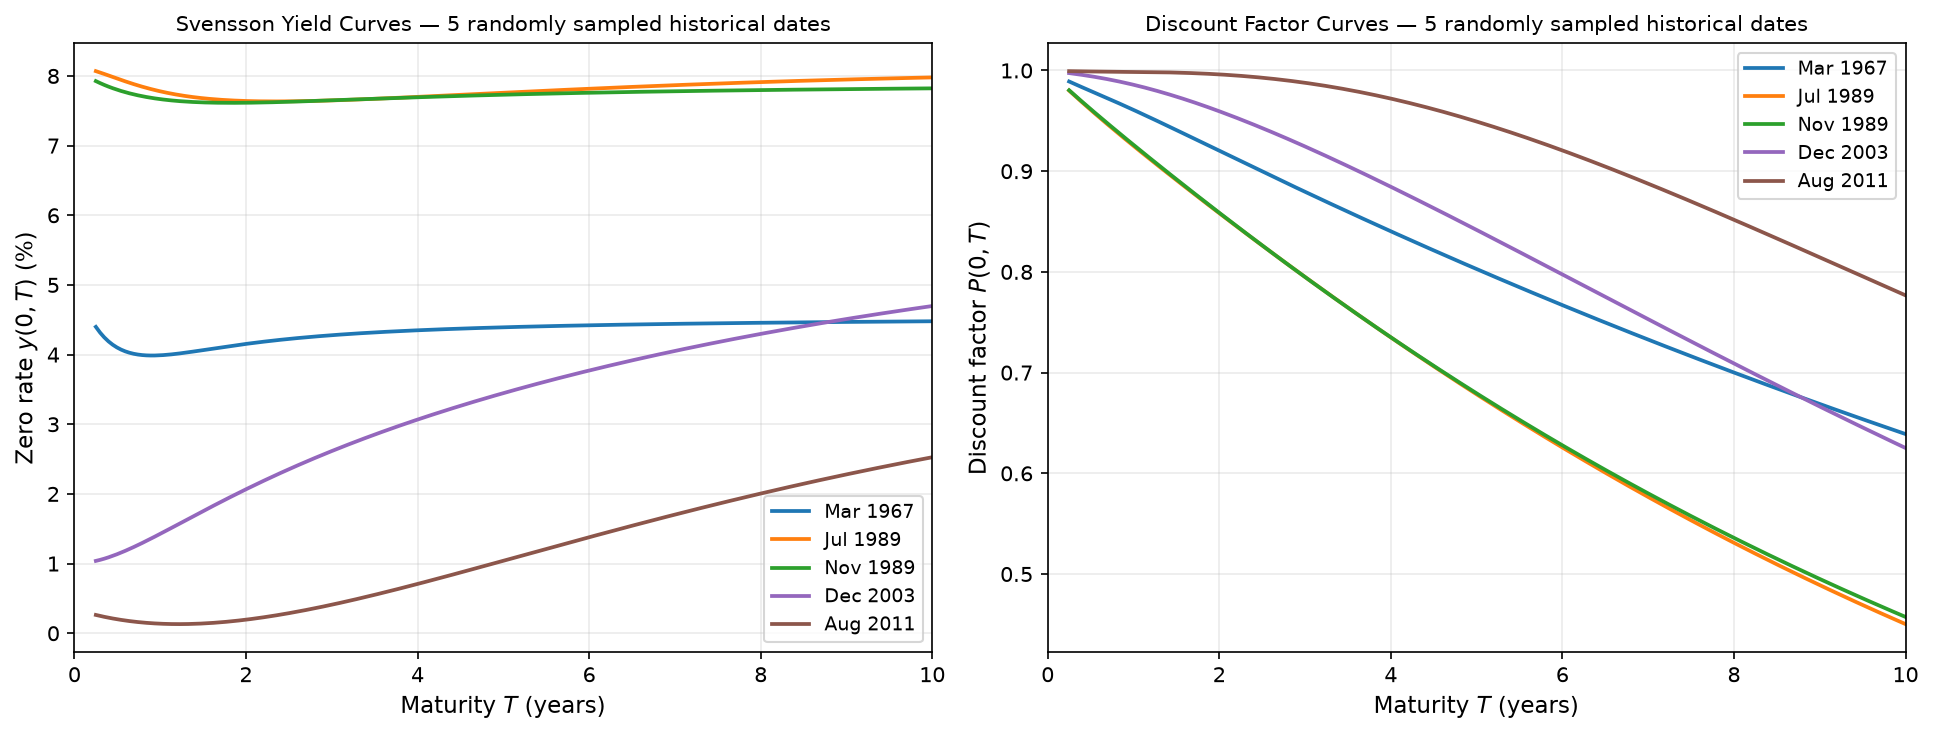
\includegraphics[width=\textwidth]{Images/b1_random_sample.png}
    \caption{Svensson yield curves (left) and corresponding discount factor curves (right)
             for five randomly sampled historical dates from the Federal Reserve GSW dataset.
             The selection illustrates the range of term structure shapes used as proxies
             for market yield curve data in this study.}
    \label{fig:random_sample_curves}
  \end{figure}

  \noindent
  The short rate evolves under the risk-neutral measure $\mathbb{Q}$ according to the Hull-White one-factor dynamics, with mean reversion speed $a > 0$ and instantaneous volatility $\sigma > 0$ both held constant over the full simulation
  horizon. The drift function $\theta(t)$ is uniquely determined by the requirement that the model reproduce the initial term structure exactly. This study does not calibrate $a$ and $\sigma$ from market-implied swaption volatilities, both are instead treated as inputs to the surrogate and sampled across a practical range, enabling the network to approximate the pricing function over a broad region of the parameter space. The simulation is initialised at the instantaneous short rate $r_0 = \lim_{T \to 0} y(0,T) = \beta_0 + \beta_1$, which is the limiting value of the Svensson zero yield as maturity approaches zero \cite{diebold2006forecasting}. \\

  \begin{figure}[H]
    \centering
    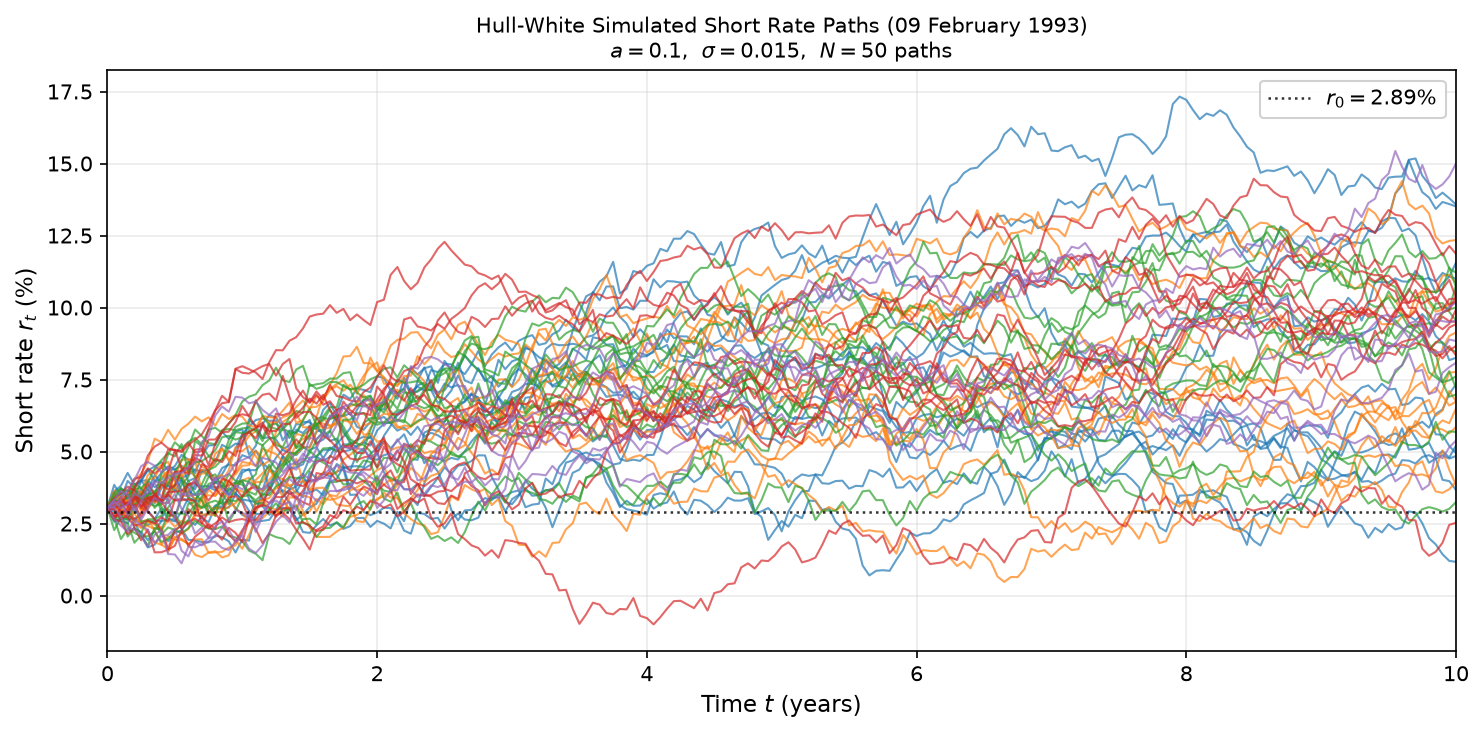
\includegraphics[width=\textwidth]{Images/b1_hw_paths.png}
    \caption{Simulated Hull-White short-rate paths over the ten-year IRS horizon,
             initialised at $r_0 = \beta_0 + \beta_1$ from the Svensson term structure.
             The upward drift of the path ensemble reflects the positive slope of the
             initial forward curve embedded in $\theta(t)$, consistent with an
             upward-sloping initial yield curve.}
    \label{fig:hw_paths}
  \end{figure}

  \noindent
  The underlying instrument is a ten-year payer IRS with semi-annual payment dates $T_j = j\tau$, $j = 1,\ldots,20$, and day count fraction $\tau = 0.5$. A single-curve framework is adopted, the same Svensson-calibrated curve is used for both discounting and floating rate estimation. No credit spread, margin, or collateral agreement is assumed. The swap is initiated at par, so $K = K^{\mathrm{par}}$ and the value at inception is zero. Notional is normalised to $N = 1$, and calendar effects are disregarded throughout. \\

  \noindent
  Monte Carlo simulation is conducted under $\mathbb{Q}$, with the short-rate process discretised via the Euler-Maruyama scheme. The simulation horizon is ten years, divided into 120 monthly steps so that monitoring dates $t_k = k/12$, $k = 0,1,\ldots,120$, align exactly with the path grid. No variance reduction techniques are employed. Training labels for the surrogate models are generated
  analytically from the Hull-White closed-form bond pricing formulae; no simulation noise enters the training data. Sensitivity labels for Model 1b are computed via automatic differentiation, not finite differences. For the xVA calculation, only unilateral CVA is considered, counterparty default is assumed independent of exposure, the hazard rate is flat, and recovery is fixed at $R = 40\%$.



  \section{Numerical Pricing of the IRS Under Hull-White}
  \label{sec:numerical_pricing}

  The computation of Credit Valuation Adjustment requires evaluating the expected positive exposure of the IRS at each date over the full life of the contract. The Expected Positive Exposure at monitoring date $t_k$ is:
  %
  \begin{equation}
    \mathrm{EPE}(t_k)
      = \mathbb{E}^{\mathbb{Q}}\!\left[
          \max\!\bigl(V_{\mathrm{IRS}}(t_k,\,r_{t_k}),\;0\bigr)
        \right]
  \end{equation}
  %
  Computing this across $N$ simulated scenarios and $K = 120$ monthly monitoring dates requires the swap value $V_{\mathrm{IRS}}(t_k, r_{t_k}^{(i)})$ at each scenario $(t_k, r_{t_k}^{(i)})$, for $i = 1,\ldots,N$ and $k = 0,\ldots,120$. This is the central pricing problem: given a future state $(t, r_t)$ with $t > 0$, determine the value of the remaining cashflows of the IRS at that state. \\

  \noindent
  Under the risk-neutral measure $\mathbb{Q}$, this value is the conditional expectation of discounted future net cashflows:
  %
  \begin{equation}
    V_{\mathrm{IRS}}(t, r_t)
      = \mathbb{E}^{\mathbb{Q}}_t\!\left[
          \sum_{j:\,T_j > t}
          \exp\!\left(-\int_t^{T_j} r_s\,\mathrm{d}s\right)\mathrm{CF}_j
        \right]
    \label{eq:rn_pricing}
  \end{equation}
  %
  where $\mathrm{CF}_j$ denotes the net cashflow at payment date $T_j$. Under the Hull-White model, this expectation admits two computationally distinct representations. The first evaluates it in closed form via the affine term structure, yielding an exact analytical price at any $(t, r_t)$. The second estimates it by Monte Carlo simulation, averaging discounted cashflows across forward paths initiated from the state $(t, r_t)$. Both representations evaluate the same expectation; the simulation estimate converges to the analytical price as the number of inner paths increases. \\

  \noindent
  This equivalence motivates the design of the two surrogate models developed in this study. Model 1a is trained to replicate the closed-form pricer, applicable wherever an analytical solution exists. Model 1b is trained to replicate the simulation-based pricer, applicable in the more general setting where no closed form is available, as is the case for multi-factor term structure models or path-dependent payoffs. Since both pricers evaluate the same underlying expectation, their convergence provides a natural validation benchmark: agreement between the two surrogate outputs confirms that each is correctly approximating the same pricing function. The two representations are described in the subsections that follow. \\

  \subsection*{Analytical Valuation: Affine Term Structure}
  \label{sec:affine_pricing}

  The initial discount factors $P(0,T_j)$ at the semi-annual payment dates are computed from the Svensson zero curve:
  %
  \begin{equation}
    P(0, T_j) = \exp\bigl(-y(0, T_j) \cdot T_j\bigr), \quad j = 1,\ldots,20
    \label{eq:df_svensson}
  \end{equation}
  %
  At a future time $t > 0$ and short rate $r_t$, each bond price is computed via the affine formula:
  %
  \begin{equation}
    P(t, T_j) = A(t, T_j)\exp\bigl(-B(t, T_j)\,r_t\bigr)
    \label{eq:hw_bond}
  \end{equation}
  %
  where:
  %
  \begin{align}
    B(t, T_j) &= \frac{1 - e^{-a(T_j - t)}}{a}
    \label{eq:hw_B} \\[4pt]
    \ln A(t, T_j) &= \ln\frac{P(0,T_j)}{P(0,t)}
      - B(t,T_j)\,f(0,t)
      - \frac{\sigma^2}{4a}\,B(t,T_j)^2\bigl(1 - e^{-2at}\bigr)
    \label{eq:hw_A}
  \end{align}
  %
  with $f(0,t)$ the initial instantaneous forward rate, approximated via central differences:
  %
  \begin{equation}
    f(0,t) \approx -\frac{\ln P(0, t+\Delta t) - \ln P(0, t-\Delta t)}{2\Delta t}
    \label{eq:fwd_finite_diff}
  \end{equation}
  %
  The payer IRS value at $(t, r_t)$ is then assembled as:
  %
  \begin{equation}
    V_{\mathrm{IRS}}(t, r_t)
      = P(t, T_0) - P(t, T_n)
        - K^{\mathrm{par}}\,\tau \sum_{j=1}^{n} P(t, T_j)
    \label{eq:irs_value}
  \end{equation}
  %
  with the par rate computed once at $t = 0$:
 
  \subsection*{Simulation-Based Valuation: Monte Carlo}
  \label{sec:mc_pricing}

  The simulation-based representation of \eqref{eq:rn_pricing} estimates the conditional expectation directly by forward simulation. Given a state $(t, r_t)$, $M$ independent short-rate paths are simulated from time $t$ to maturity $T_n$ via the Euler-Maruyama scheme: 
  %
  \begin{equation}
    r_{s+\Delta s}^{(i)}
      = r_s^{(i)}
        + \bigl(\theta(s) - a\,r_s^{(i)}\bigr)\Delta s
        + \sigma\,\sqrt{\Delta s}\,Z_s^{(i)},
    \quad Z_s^{(i)} \sim \mathcal{N}(0,1)
    \label{eq:euler_maruyama}
  \end{equation}
  %
  On each path $i$, the net cashflow at remaining payment date $T_j > t$ is:
  %
  \begin{equation}
    \mathrm{CF}_j^{(i)}
      = \left(\frac{1}{P\!\left(T_{j-1},\,T_j \mid r_{T_{j-1}}^{(i)}\right)} - 1\right)
        - K^{\mathrm{par}}\tau
    \label{eq:mc_cf}
  \end{equation}
  %
  where $P(T_{j-1}, T_j \mid r_{T_{j-1}}^{(i)})$ is the affine bond price
  evaluated at the simulated short rate $r_{T_{j-1}}^{(i)}$. Each cashflow
  is discounted to $t$ using the path numeraire:
  %
  \begin{equation}
    D^{(i)}(t,\,T_j)
      = \exp\!\left(-\sum_{s:\,t \leq s < T_j} r_s^{(i)}\,\Delta s\right)
    \label{eq:path_disc}
  \end{equation}
  %
  The simulation-based swap value is then:
  %
  \begin{equation}
    V_{\mathrm{MC}}(t, r_t)
      = \frac{1}{M}\sum_{i=1}^{M}\;\sum_{j:\,T_j > t}
          \mathrm{CF}_j^{(i)}\,D^{(i)}(t,\,T_j)
    \label{eq:irs_mc}
  \end{equation}
  %
  By the risk-neutral pricing theorem, $V_{\mathrm{MC}}$ is an unbiased estimator of $V_{\mathrm{affine}}$, and the two converge as $M \to \infty$. This is the pricing method replicated by Model 1b.

  \section{Monte Carlo Simulation and Exposure}
  \label{sec:mc_exposure}

  The expected exposure profiles are computed by simulation across $N$
  independent outer paths. For each path $i = 1,\ldots,N$, the short rate
  is evolved from $t = 0$ to $T_n$ via \eqref{eq:euler_maruyama} over
  $K = 120$ monthly monitoring dates $t_k = k/12$, $k = 0,1,\ldots,120$.
  At each scenario $(i, t_k)$, the swap value $V_{\mathrm{IRS}}(t_k,
  r_{t_k}^{(i)})$ is evaluated using the appropriate pricer. The Expected
  Positive Exposure and Expected Negative Exposure profiles are:
  %
  \begin{align}
    \mathrm{EPE}(t_k)
      &= \frac{1}{N}\sum_{i=1}^{N}
           \max\!\bigl(V_{\mathrm{IRS}}(t_k,\,r_{t_k}^{(i)}),\;0\bigr)
      \label{eq:epe} \\[4pt]
    \mathrm{ENE}(t_k)
      &= \frac{1}{N}\sum_{i=1}^{N}
           \min\!\bigl(V_{\mathrm{IRS}}(t_k,\,r_{t_k}^{(i)}),\;0\bigr)
      \label{eq:ene}
  \end{align}
  %
  These profiles feed directly into the CVA calculation in
  Section~\ref{sec:xva}. In the surrogate-based calculation,
  $V_{\mathrm{IRS}}(t_k, r_{t_k}^{(i)})$ is replaced by the surrogate
  output $\hat{V}(t_k, r_{t_k}^{(i)})$, reducing each scenario valuation
  to a single network forward pass. The accuracy of this substitution,
  measured by the gap between the surrogate-based and reference EPE profiles,
  is one of the primary evaluation criteria in the Results chapter.


  %==============================================================================
  \section{Surrogate Models}
  \label{sec:surrogates}
  %==============================================================================

  Three surrogate models are developed to approximate IRS pricing within the
  Monte Carlo CVA pipeline. Each replaces calls to the reference pricer with a
  single forward pass of a trained network. The models share a common GRU
  architecture but differ in their training data sources and loss functions,
  enabling a controlled comparison of the effects of data origin and sensitivity
  supervision on surrogate accuracy.

  \subsection{Data Generation}
  \label{sec:data_gen}

  Training corpora for the three models are constructed as follows. \\

  \noindent
  \textbf{Model 1a.} Training inputs $(a, \sigma, t, r_t)$ are sampled from a
  designed grid spanning a practical parameter range: $a \in [0.01, 0.30]$,
  $\sigma \in [0.005, 0.030]$, $t \in \{t_k\}_{k=0}^{120}$, and $r_t$ drawn
  uniformly around the initial short rate. Price labels
  $V^* = V_{\mathrm{affine}}(t, r_t; a, \sigma)$ are computed from the
  closed-form formula \eqref{eq:irs_value}. No sensitivity labels are generated. \\

  \noindent
  \textbf{Model 1b.} Training scenarios $(t_k, r_{t_k}^{(i)})$ are extracted
  directly from the outer Monte Carlo paths used in the CVA computation described
  in Section~\ref{sec:mc_exposure}. This in-distribution design ensures the
  surrogate is trained on the same domain of short-rate realisations it encounters
  at evaluation time. Price labels $V^* = V_{\mathrm{MC}}(t_k, r_{t_k}^{(i)})$
  are computed via the simulation-based pricer \eqref{eq:irs_mc}. No sensitivity
  labels are generated. \\

  \noindent
  \textbf{Model 2.} Training scenarios are the same simulation-drawn pairs as
  Model 1b. Price labels are likewise from the simulation-based pricer. In
  addition, key-rate DV01 labels:
  %
  \begin{equation}
    \mathrm{DV01}_k^* = \frac{\partial V_{\mathrm{MC}}}{\partial y_k},
    \quad k = 0, 1, \ldots, 9
    \label{eq:dv01_label}
  \end{equation}
  %
  are computed by automatic differentiation through the simulation pricing
  function, following \cite{huge2020differential}. These sensitivity labels are
  used jointly with the price labels in the Sobolev training objective described
  in Section~\ref{sec:training_objectives}.

  \subsection{Model Inputs}
  \label{sec:model_inputs}

  All three models receive the same input representation. The primary sequence is
  a vector of zero yields $\{y(0, T_k)\}_{k=1}^{10}$ at ten tenor knot points
  spanning three months to ten years, providing a discretised snapshot of the
  prevailing term structure. A scalar vector $(a, \sigma, t, r_t)$ supplies the
  Hull-White parameters and the current state. Yield curve values are used as the
  sequence input rather than discount factors because the DV01 labels in Model 2
  are defined as derivatives with respect to yields; providing yields directly
  ensures that the gradient $\partial\hat{V}/\partial y_k$ obtained by
  backpropagation is well-defined and numerically stable across all three models.

  \subsection{Architecture}
  \label{sec:architecture}

  A single GRU architecture is used for all three models without structural
  modification between them. The network processes the ten-element yield sequence
  through $L$ stacked GRU layers, whose update, reset, candidate, and hidden-state
  equations are given in \eqref{eq:gru_update}--\eqref{eq:gru_hidden} of the
  Theoretical Foundations. The final hidden state $\mathbf{h}_{10} \in
  \mathbb{R}^H$ is concatenated with the scalar input vector $(a, \sigma, t, r_t)$
  and passed through a linear output layer to produce the predicted swap value
  $\hat{V}$. Sensitivity outputs $\partial\hat{V}/\partial y_k$ are obtained by
  backpropagation through the network at inference time, requiring no architectural
  modification. The same network can therefore be trained under any of the three
  loss functions in Section~\ref{sec:training_objectives} without alteration. A
  depth of $L = 2$ layers and hidden dimension $H = 64$ are used as the base
  configuration, reflecting the low intrinsic dimensionality of the pricing
  function under the one-factor Hull-White model; these are verified by grid search
  on the validation set.

  \subsection{Training Objectives}
  \label{sec:training_objectives}

  The three models are distinguished solely by their loss functions. \\

  \noindent
  \textbf{Model 1a} minimises the mean squared error on the analytical price
  labels:
  %
  \begin{equation}
    \mathcal{L}_{1a}
      = \frac{1}{M}\sum_{m=1}^{M}
          \bigl(\hat{V}_m - V_{\mathrm{affine},m}^*\bigr)^2
    \label{eq:loss_1a}
  \end{equation}

  \noindent
  \textbf{Model 1b} minimises the mean squared error on the simulation price
  labels:
  %
  \begin{equation}
    \mathcal{L}_{1b}
      = \frac{1}{M}\sum_{m=1}^{M}
          \bigl(\hat{V}_m - V_{\mathrm{MC},m}^*\bigr)^2
    \label{eq:loss_1b}
  \end{equation}

  \noindent
  \textbf{Model 2} minimises a Sobolev loss that penalises errors in both price
  and sensitivities jointly \cite{huge2020differential}:
  %
  \begin{equation}
    \mathcal{L}_{2}
      = \frac{1}{M}\sum_{m=1}^{M}\left[
          \bigl(\hat{V}_m - V_{\mathrm{MC},m}^*\bigr)^2
          + \lambda\sum_{k=0}^{9}
            \!\left(
              \frac{\partial\hat{V}_m}{\partial y_k}
              - \mathrm{DV01}_{k,m}^*
            \right)^{\!2}
        \right]
    \label{eq:loss_2}
  \end{equation}
  %
  The weight $\lambda > 0$ balances the price and sensitivity terms. Its
  magnitude is informed by the ratio of the typical price error to the typical
  DV01 error on the validation set; values in the range $\lambda \in [0.1, 1.0]$
  are evaluated by grid search. All three models are optimised using the Adam
  algorithm \cite{kingma2015adam} with an initial learning rate of $10^{-3}$ and
  a cosine annealing schedule. Training, validation, and test sets are constructed
  from disjoint subsets of the generated data; early stopping on validation loss
  selects the final checkpoint.


  %==============================================================================
  \section{xVA Calculation}
  \label{sec:xva}
  %==============================================================================

  The surrogate models are designed for a specific purpose: to replace the
  analytical Hull-White pricer at each simulated scenario in a Monte Carlo-based
  CVA calculation. CVA measures the market value of counterparty default risk, and
  computing it requires repricing the swap across the full set of simulated future
  scenarios. At production scale, this repricing step dominates the computational
  cost; replacing the analytical pricer with a trained surrogate reduces each
  scenario valuation to a single forward pass of fixed cost.

  Under the assumptions of Section~\ref{sec:assumptions}, the unilateral CVA is:
  %
  \begin{equation}
  \mathrm{CVA}
    = (1 - R)\int_0^{T_n}
      \mathrm{EPE}(t)\,\lambda\,e^{-(\lambda + r_0)t}\,\mathrm{d}t
  \label{eq:cva}
  \end{equation}
  %
  where $R = 0.40$ is the recovery rate, $\lambda$ is the constant hazard rate,
  $r_0$ is the initial short rate, and $\mathrm{EPE}(t)$ is the expected positive
  exposure profile from Section~\ref{sec:mc_exposure}. Discretising over the 120
  monthly monitoring dates:
  %
  \begin{equation}
  \mathrm{CVA}
    \approx (1 - R)\sum_{k=1}^{120}
      \mathrm{EPE}(t_k)\,\lambda\,e^{-(\lambda + r_0)t_k}\,\Delta t
  \label{eq:cva_discrete}
  \end{equation}
  %
  where $\Delta t = 1/12$. In the surrogate-based calculation, the EPE profile is
  constructed by replacing $V_{\mathrm{IRS}}^{(i)}(t_k, r_{t_k}^{(i)})$ in
  \eqref{eq:epe} with the surrogate output $\hat{V}^{(i)}(t_k)$. The gap between
  surrogate-based CVA and analytical CVA is a direct measure of the pricing error
  that accumulates across the full exposure simulation, and is one of the primary
  metrics used to compare Model 1a and Model 1b in the Results chapter.

        

\part{Results and Analysis}
    

       

\part{Conclusion and Future Work}

    
\appendix
\part{Appendices}
    \chapter{Mathematical Proofs and Derivations}
        
    \chapter{Code Implementation Details}
        
    \chapter{Additional Numerical Results}
      

%-------------------------------------------------------------------------------
% REFERENCES
%-------------------------------------------------------------------------------
\newpage
\bibliography{mybibliography}
\addcontentsline{toc}{part}{References}


\end{document}